\documentclass[lettersize,journal]{IEEEtran}

\usepackage{cite}
\usepackage[T1]{fontenc}
\usepackage{amsmath,amsfonts,amssymb,bm}
\usepackage{algorithmic}
\usepackage{algorithm}
\usepackage{array}
\usepackage[caption=false,font=normalsize,labelfont=sf,textfont=sf]{subfig}
\usepackage{textcomp}
\usepackage{stfloats}
\usepackage{url}
\usepackage{verbatim}
\usepackage{graphicx}
\usepackage{booktabs}
\usepackage{multirow}
\usepackage{mathtools}
\usepackage{float}
\usepackage{placeins}
\usepackage{caption}
%\usepackage[backend=biber,style=ieee,sorting=none]{biblatex}
%\addbibresource{references.bib}

\newcommand{\vect}[1]{\boldsymbol{#1}}
\newcommand{\mat}[1]{\mathbf{#1}}
\newcommand{\R}{\mathbb{R}}
\newcommand{\C}{\mathbb{C}}
\newcommand{\od}{\odot}
\newcommand{\norm}[1]{\left\lVert #1 \right\rVert}
\newcommand{\argmin}{\mathop{\mathrm{arg\,min}}}
\DeclareMathOperator{\softplus}{softplus}
\DeclareMathOperator{\Concat}{Concat}
\DeclareMathOperator{\logten}{log_{10}}
\DeclareMathOperator{\Conv}{Conv}
\DeclareMathOperator{\GN}{GN}
\DeclareMathOperator{\SiLU}{SiLU}
\DeclareMathOperator{\Linear}{Linear}
\DeclareMathOperator{\Dropout}{Dropout}
\DeclareMathOperator{\Skip}{Skip}
\DeclareMathOperator{\Res}{Res}
\DeclareMathOperator{\Down}{Down}
\DeclareMathOperator{\Up}{Up}
\DeclareMathOperator{\Attn}{Attn}
\DeclareMathOperator{\Head}{Head}
\DeclareMathOperator{\BN}{BN}
\DeclareMathOperator{\ReLU}{ReLU}
\DeclareMathOperator{\CBR}{CBR}
\DeclareMathOperator{\Enc}{Enc}
\DeclareMathOperator{\Dec}{Dec}
\DeclareMathOperator{\Interp}{Interp}

\begin{document}

\title{PIDR-Net: A Physics Informed Diffusion Refinement Network for Channel Map Estimation in Movable Antenna Systems}

\author{Authors}

\markboth{Journal of \LaTeX\ Class Files,~Vol.~14, No.~8, August~2021}%
{Anonymous \MakeLowercase{\textit{et al.}}: PIDR-Net for Channel Map Estimation in Movable Antenna Systems}

\maketitle

\begin{abstract}
Movable antenna (MA) has attracted increasing attention in wireless communications due to its capability of wireless channel reconfiguration through local antenna movement within a confined region at the transmitter/receiver. However, to determine the optimal antenna positions, channel state information (CSI) within the entire region, termed small-scale channel map, is required, which poses a significant challenge due to the unaffordable overhead for exhaustive channel estimation at all positions. Unlike existing works assuming a theoretical channel model for channel map reconstruction, this paper investigates a data-driven approach based on practical channel models. Specifically, a physics informed diffusion refinement network, termed PIDR-Net, is proposed to reconstruct the channel map within a two-dimensional (2D) MA movement region from channel estimates at a small subset of positions. Specifically, PIDR-Net first reconstructs the unmeasured entries with a conditional denoising diffusion model. During reverse sampling, it restores the measured values after each step and periodically recomputes the amplitude channel from the real and imaginary channels. A compact refinement network then corrects the diffusion estimate using the observation mask, grid coordinates, and a learned radial template for attenuation and phase. Extensive simulation results are provided to show the efficacy of our proposed PIDR-Net over other benchmark schemes under various practical channel models and also unveil the impacts of measurement antenna positions and budgets, on the overall performance
\end{abstract}

\begin{IEEEkeywords}
Movable antennas, channel map estimation, diffusion model, physics-informed neural network.
\end{IEEEkeywords}


\section{Introduction}

Increasing the number of antenna elements improves spatial multiplexing, beamforming gain, and interference suppression in modern wireless systems. Conventional multiple-input multiple-output (MIMO) architectures have evolved toward massive MIMO in fifth generation networks and may scale further to extremely large scale MIMO and ultra massive arrays in sixth generation systems \cite{ref_xlmimo_tutorial,ref_ultra_massive_beamforming,ref_near_far_field}. Larger arrays also require more radio frequency hardware, calibration, physical aperture, and energy \cite{ref_ultra_massive_beamforming,ref_near_far_field}. These costs motivate methods that exploit spatial diversity without adding more fixed antenna elements.

Movable antenna (MA) technology offers one such method. An MA can move within a confined region and select a position with favorable propagation conditions \cite{ref_ma_opportunities,ref_ma_modeling}. Existing studies report gains in spectral efficiency, beam coverage, security, and performance for multiple users with fewer antenna elements than comparable architectures with fixed antennas \cite{ref_ma_multiuser,ref_ma_graph,ref_ma_spectrum,ref_ma_beam_coverage,ref_ma_security}. The resulting channel depends on the selected MA position, so position selection requires knowledge of the spatial channel variation within the movement region.

Beamforming, user scheduling, antenna position selection, and movement planning depend on the CSI at both sounded and unsounded candidate positions. The transmitter therefore needs a local channel map over the small movement region \cite{ref_ma_modeling}. Measuring every candidate position requires pilot overhead proportional to the number of grid points and increases acquisition time. This paper reconstructs complex CSI rather than gain alone because the amplitude, real, and imaginary components are algebraically related and are all needed for antenna selection and coherent transmission.

Existing MA channel estimation and mapping studies use compressed sensing \cite{ref_cs,ref_cs_framework}, Bayesian sparse reconstruction \cite{ref_sbar}, learning methods \cite{ref_agmae}, and tensor decomposition for MIMO MA systems \cite{ref_tensor}. Much of this work estimates a real valued gain map, whereas communication design may also require the real and imaginary components that contain the phase information. In addition, deterministic regressors trained from sparse inputs can lose accuracy when measurements are scarce, irregularly distributed, or confined to one part of the grid, where values outside the measured region must be extrapolated.

Sparse MA channel map estimation must fill large unmeasured regions while preserving the relations among the three CSI channels. Denoising diffusion models can learn the distribution of complete maps and generate missing values conditioned on partial observations \cite{ref_ddpm}. After this initial estimate, propagation features and algebraic channel relations can be used to correct local errors. Physics informed neural networks (PINNs) provide a way to include such information in a learned reconstruction model \cite{ref_pinn}. We therefore use diffusion for the initial map estimate and a PINN for the subsequent correction.

This paper studies sparse complex CSI map reconstruction over a 2D MA movement region and proposes PIDR-Net for this task. Its conditional diffusion stage estimates the complete map from sparse CSI observations. During reverse sampling, measured entries are restored after each step, and the amplitude channel is periodically recomputed from the real and imaginary channels. A compact PINN then refines the estimate using the diffusion output, observation mask, coordinate tensor, and a learned propagation prior. The two stages are trained separately and perform initial reconstruction followed by local correction.

The main contributions of this paper are summarized as follows.
\begin{itemize}
    \item We formulate sparse complex CSI reconstruction for an MA system as a map completion problem with three channels on a 2D movement region, with observation masking, validity screening, and separate normalization of the amplitude, real, and imaginary components.
    \item We propose a conditional diffusion stage that reconstructs complete CSI maps by reverse sampling with exact restoration of measured values and periodic correction of the amplitude channel.
    \item We design a lightweight physics informed refinement stage that incorporates coordinate features and a learnable propagation prior into a reconstruction network with an encoder and decoder.
    \item We develop separate training  and inference procedures for the two stages, reuse diffusion estimates during refiner training, and evaluate PIDR-Net on RT and two additional datasets, multiple sampling strategies and measurement budgets, and MA position optimization.
\end{itemize}

The remainder of this paper is organized as follows. Section~\ref{sec:problem} introduces the MA system model and hybrid estimation protocol. Section~\ref{sec:method} describes offline measurements, data processing, the two PIDR-Net stages, and their training and inference procedures. Section~\ref{sec:exp} reports the experimental setup and benchmark results on three datasets. Section~\ref{sec:conclusion} concludes the paper.

\section{System Model and Estimation Protocol}
\label{sec:problem}

\subsection{System Model}

As shown in Fig.~\ref{fig:ma_system_model}, we consider an MA system where a base station (BS) equipped with $L$ movable antennas (MAs) communicates with a single-FPA user. Each MA can move within a confined 2D square transmit region $\mathcal{C}_{\mathrm t}\subset\R^{2\times 1}$. Let $D_{\mathrm t}\lambda$ denote the side length of $\mathcal{C}_{\mathrm t}$, where $\lambda$ is the carrier wavelength and $D_{\mathrm t}$ is the normalized side length. For convenience, a 2D Cartesian coordinate system is introduced for the transmit region, with the origin denoted by $\vect{o}_{\mathrm t}=[0,0]^T$. The figure distinguishes pilot transmission to channel measurement devices at locations $\vect{r}_1,\vect{r}_2,\ldots,\vect{r}_S$ from data transmission to the user.

\begin{figure*}[!t]
    \centering
    \captionsetup{font=footnotesize}
    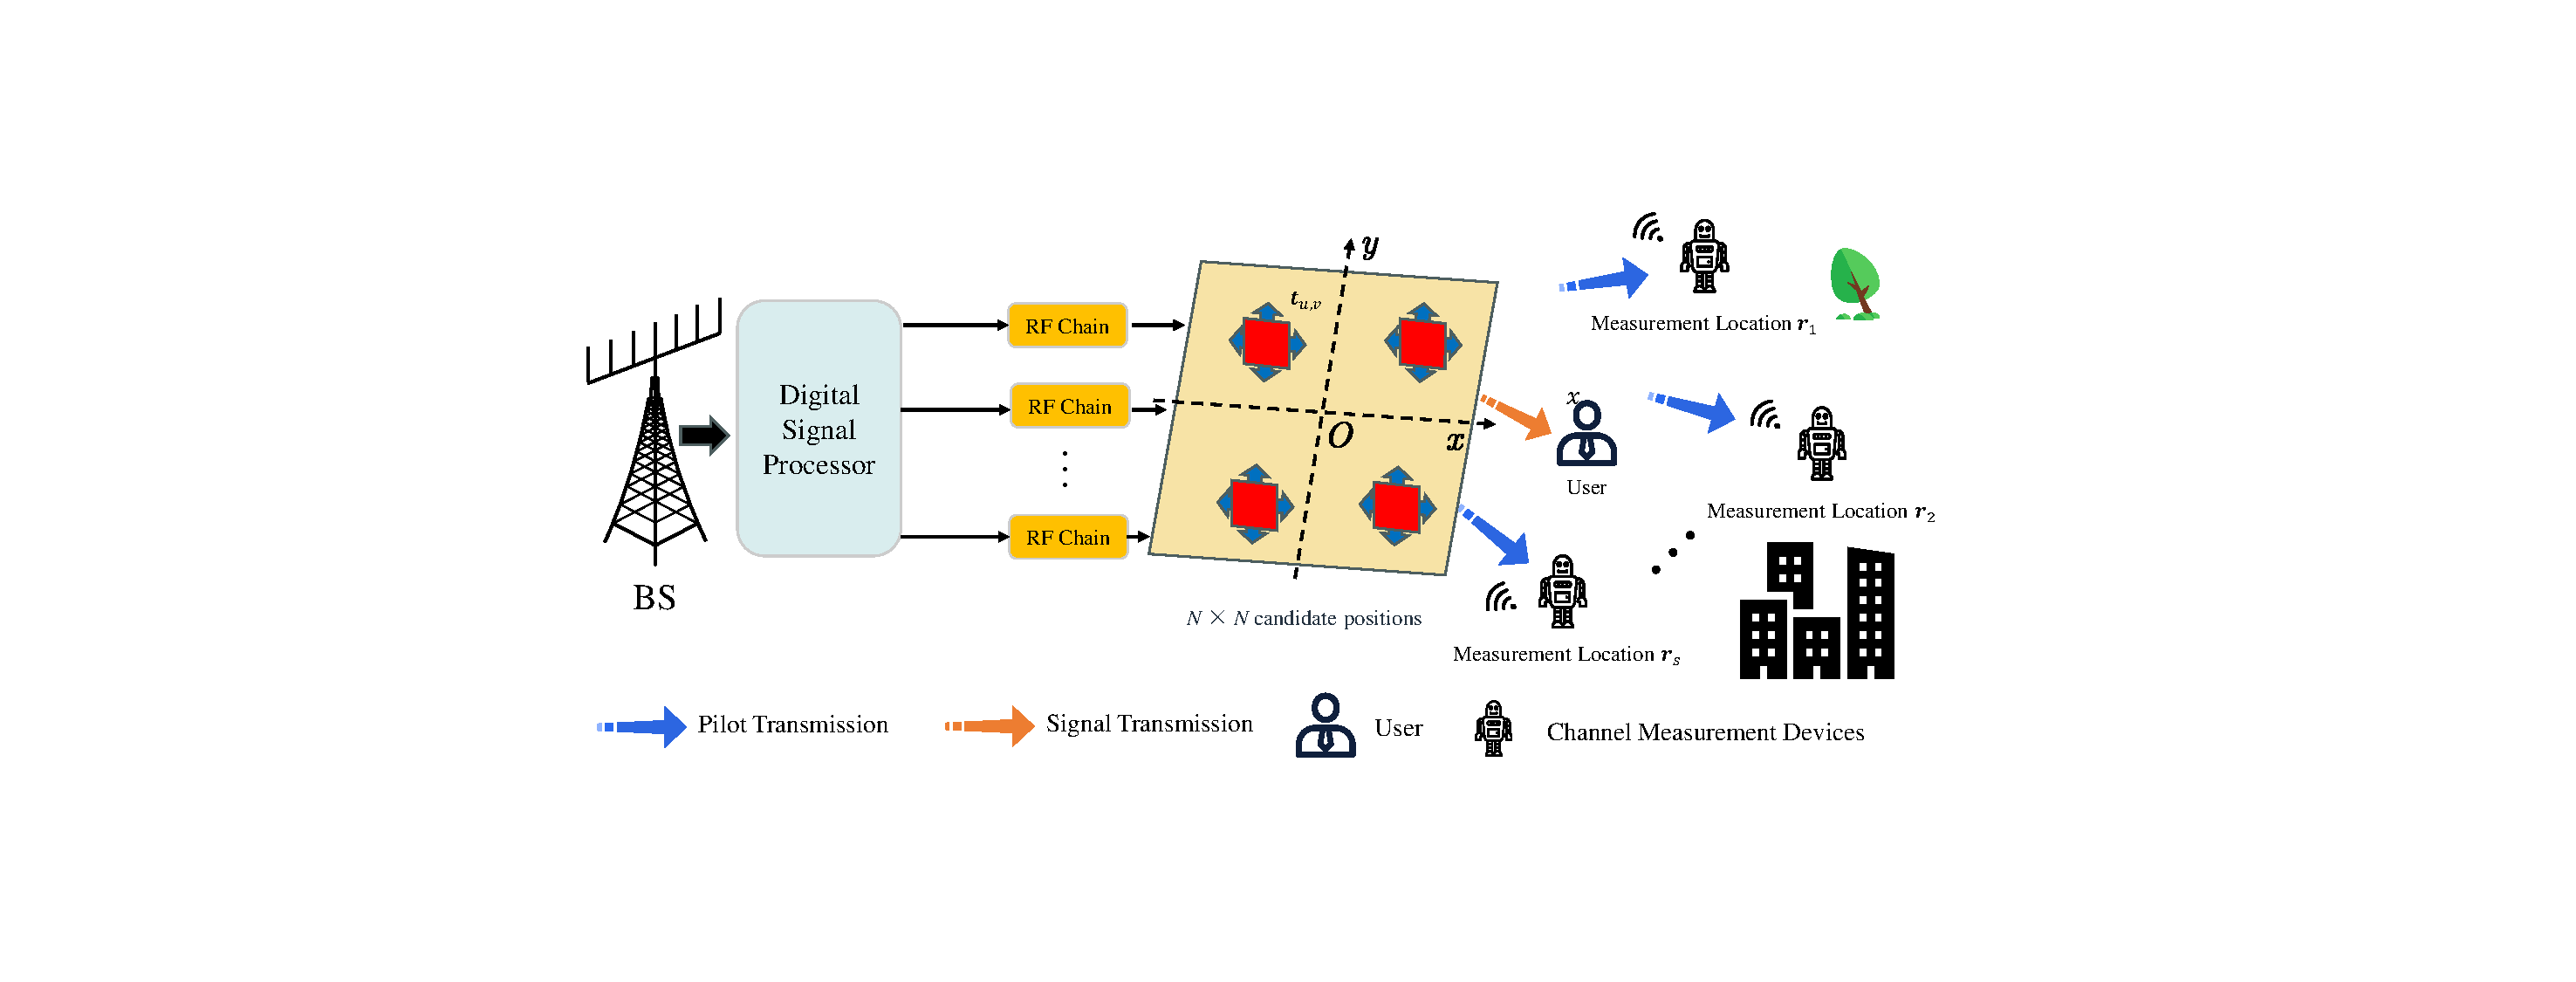
\includegraphics[width=0.94\textwidth]{figures/ma_system_model.pdf}
    \caption{\protect\centering MA downlink with pilot based channel measurements and user data transmission.}
    \label{fig:ma_system_model}
\end{figure*}

As indicated in Fig.~\ref{fig:ma_system_model}, each of the $L$ MAs can move among $N\times N$ candidate positions in the transmit region. A channel measurement device is placed at $\vect{r}_s$ to collect one offline map: it receives pilots as the BS sounds selected MA positions. The device remains at $\vect{r}_s$ for that map and is relocated between collection rounds. The user shown in the figure is distinct from these offline measurement devices; during online operation, the user can also receive pilots at a small subset of MA positions before data transmission.

Let $\vect{t}\in\mathcal{C}_{\mathrm t}$ denote the MA's position. We suppress the receiver index when discussing one map. The complex channel coefficient associated with an MA at $\vect{t}$ is
\begin{equation}
    h(\vect{t})=h^{\mathrm{re}}(\vect{t})+j h^{\mathrm{im}}(\vect{t}),
    \label{eq:continuous_channel_t}
\end{equation}
where $h^{\mathrm{re}}(\vect{t})$ and $h^{\mathrm{im}}(\vect{t})$ denote its real and imaginary parts, respectively. The corresponding channel amplitude in decibels (dB) is
\begin{equation}
    g(\vect{t})=10\log_{10}\!\left(\sqrt{\big(h^{\mathrm{re}}(\vect{t})\big)^2+\big(h^{\mathrm{im}}(\vect{t})\big)^2}\right),
    \label{eq:continuous_gain_t}
\end{equation}

To facilitate practical channel map construction, the continuous region ${\cal C}_t$ is discretized into $N\times N$ grids.. Each spatial dimension has $N$ uniformly spaced points, giving a sampling interval of
\begin{equation}
    \Delta_{\mathrm t}=\frac{D_{\mathrm t}\lambda}{N-1}.
    \label{eq:grid_spacing}
\end{equation}
Let $\vect{t}_{u,v}\in\mathcal{C}_{\mathrm t}$ denote the position of grid point $(u,v)$-th sampling point, with $1\le u,v\le N$. Then, the resulting 2D channel map is
\begin{equation}
    \mathcal{H}=\left\{h(\vect{t}_{u,v})\,\middle|\,1\le u,v\le N\right\}.
    \label{eq:channel_map_set}
\end{equation}
Under the adopted position dependent channel model, the coefficient at a grid point does not depend on which of the $L$ MAs is used to measure it. Thus, a single map is defined for each receiver location.

For learning and inference purposes, the channel map in \eqref{eq:channel_map_set} is stored as a three-channel tensor given by
\begin{equation}
    \mat{X}\in\R^{3\times N\times N},
    \qquad
    \mat{X}=\big[\mat{X}^{\mathrm a},\mat{X}^{\mathrm{re}},\mat{X}^{\mathrm{im}}\big],
    \label{eq:X_complete}
\end{equation}
where $\mat{X}^{\mathrm a}(u,v)=g(\vect{t}_{u,v})$, $\mat{X}^{\mathrm{re}}(u,v)=h^{\mathrm{re}}(\vect{t}_{u,v})$, and $\mat{X}^{\mathrm{im}}(u,v)=h^{\mathrm{im}}(\vect{t}_{u,v})$ for all $1\le u,v\le N$.

For offline data collection, let $\mathcal{R}_{\mathrm{off}}=\{\vect{r}_s\mid 1\le s\le S\}$ denote a set of $S$ receiver locations in the deployment environment. The underlying channel map at $\vect{r}_s$ is denoted by $\mat{X}^{(s)}$, an instance of $\mat{X}$ in \eqref{eq:X_complete}. Its values are defined over the full grid, but only the positions in a measured set $\mathcal{A}_s\subseteq\Omega$, where $\Omega=\{1,\ldots,N\}\times\{1,\ldots,N\}$, are available in the offline sample. We denote the resulting measured tensor by $\mat{X}_s$: it contains the measured values on $\mathcal{A}_s$ and zeros at unsounded positions. Thus, $\mat{X}_s$ is a complete measured map only if $\mathcal{A}_s=\Omega$.

\subsection{Hybrid Offline/Online Estimation Protocol}

Notably, a straightforward method for estimating the channel map in \eqref{eq:channel_map_set} is to sound all $N^2$ grid centers within $\mathcal{C}_{\mathrm t}$. However, this would incur substantial pilot overhead, MA movement cost, and latency during online operation. Therefore, we adopt a hybrid offline/online estimation protocol.

The offline stage sends pilots from selected transmit MA positions to channel measurement devices at multiple receiver locations to build samples for training. Section~\ref{sec:offline_measurements} describes how these measurements are acquired and organized.

During online operation, only a small subset of transmit MA positions is sounded for the current user. The resulting partial measurements are processed by the pretrained reconstruction model to infer the complete channel map. The reconstructed map supports antenna position selection for subsequent data transmission, while the limited sounding reduces online pilot overhead and MA movement.

To this end, we define a binary input mask $\mat{M}^{I}\in\{0,1\}^{N\times N}$, where $M^{I}(u,v)=1$ if the CSI at $(u,v)$ is supplied to the reconstruction model and $0$ otherwise. During training, a separate binary mask $\mat{M}^{L}$ identifies the positions available as labels. Both masks are shared by the three CSI channels, but the label mask is not an input to the model. For a channel map $\mat{X}$, the input and label tensors are
\begin{equation}
    \mat{X}^{I}=\mat{X}\od\mat{M}^{I},\qquad
    \mat{X}^{L}=\mat{X}\od\mat{M}^{L},
    \label{eq:input_label_maps}
\end{equation}
where $\od$ denotes the Hadamard product. In an offline sample, the corresponding relations are $\mat{X}_s^{I}=\mat{X}_s\od\mat{M}_s^{I}$ and $\mat{X}_s^{L}=\mat{X}_s\od\mat{M}_s^{L}$; the masks may differ across samples, and label positions must lie in $\mathcal{A}_s$.

The reconstruction task is to estimate the underlying channel map from the input pair $(\mat{X}^{I},\mat{M}^{I})$ according to
\begin{equation}
    \widehat{\mat{X}}=\mathcal{F}(\mat{X}^{I},\mat{M}^{I}),
    \label{eq:task}
\end{equation}
where $\mathcal{F}$ is modeled by the proposed PIDR-Net in Section~\ref{sec:method}. The label pair $(\mat{X}^{L},\mat{M}^{L})$ is used only to evaluate training losses; it is not required during online reconstruction.

Fig.~\ref{fig:offline_online_protocol} summarizes the proposed estimation protocol. The offline branch acquires channel measurements at different receiver locations, processes their amplitude, real part, and imaginary part, and uses them to train PIDR-Net. The online branch acquires measurements at selected MA positions to form $(\mat{X}^{I},\mat{M}^{I})$ and then applies the pretrained model to reconstruct the complete channel map.

\begin{figure}[t]
    \centering
    \captionsetup{font=footnotesize}
    % Replace the file path below with the final protocol flowchart path.
    \IfFileExists{figures/offline_online_protocol.pdf}{
        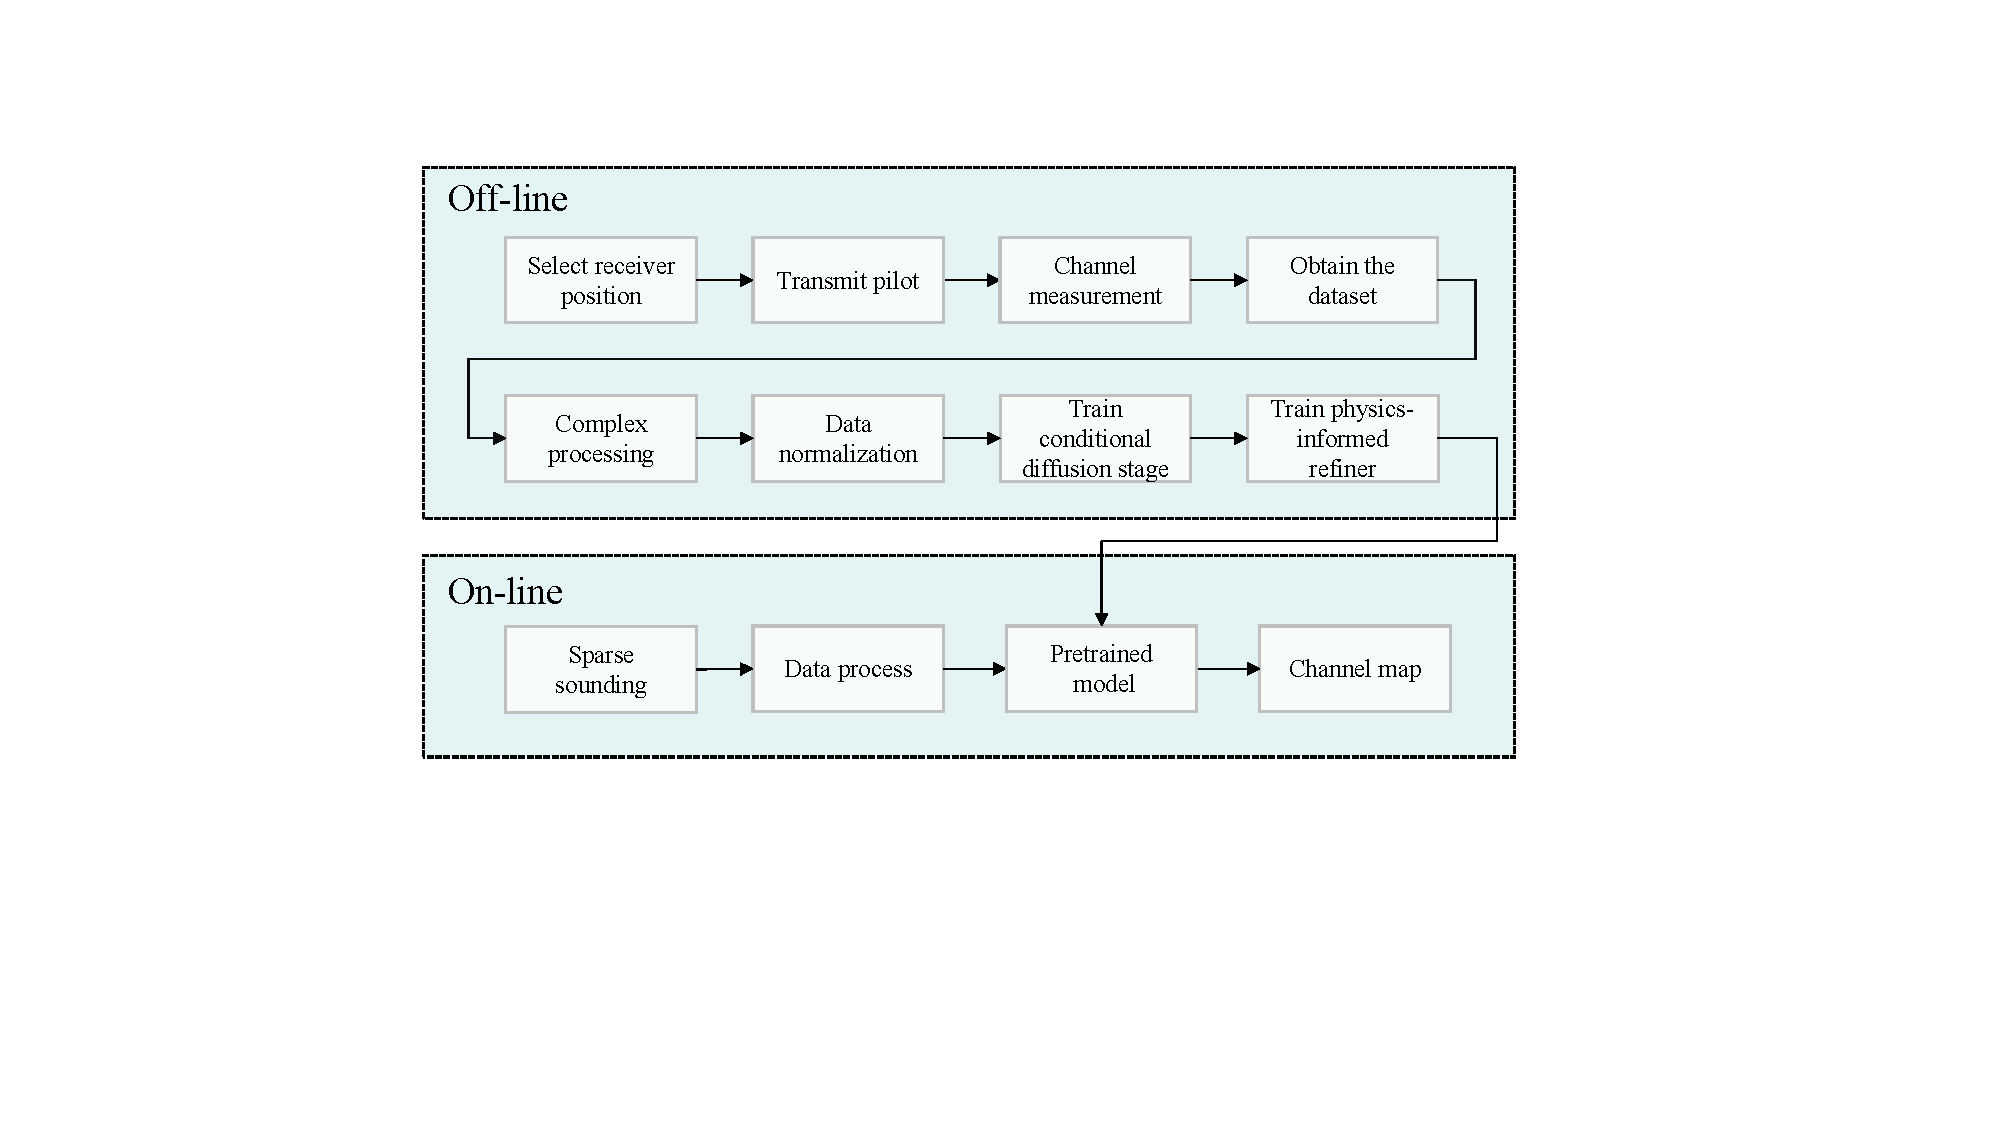
\includegraphics[width=\columnwidth]{figures/offline_online_protocol.pdf}
    }{
        \fbox{\parbox[c][0.15\textheight][c]{0.92\columnwidth}{\centering Offline/online protocol flowchart placeholder}}
    }
    \caption{\protect\centering Hybrid offline/online channel map estimation protocol.}
    \label{fig:offline_online_protocol}
\end{figure}


\section{Proposed PIDR-Net Algorithm for Channel Map Estimation}
\label{sec:method}

This section presents the architecture of our proposed PIDR-Net for channel map estimation which includes the conditional diffusion stage, the physics informed refinement stage, and their training and inference procedures.

\subsection{Offline Channel Measurements}
\label{sec:offline_measurements}

In an offline collection procedure, a single-antenna channel measurement device can be mounted on a mobile robot and placed successively at the locations in $\mathcal{R}_{\mathrm{off}}$. For each robot's measurement location $\vect{r}_s$, the device remains stationary while the BS sounds the selected grid points $\mathcal{A}_s\subseteq\Omega$.\footnote{As there are L transmit MAs, we can measure the channels for L MA training position each time.} The robot relocates the device between collection rounds.

At each $(u,v)\in\mathcal{A}_s$, the BS sends a pilot with its MA at $\vect{t}_{u,v}$, and the measurement device estimates the complex coefficient $h_s(\vect{t}_{u,v})$ for the link to $\vect{r}_s$. The measurements for this receiver location form one sample, and the offline measurement dataset can be written as
\begin{equation}
    \mathcal{D}_{\mathrm{off}}=
    \left\{\left(\mathcal{A}_s,
    \{h_s(\vect{t}_{u,v})\}_{(u,v)\in\mathcal{A}_s}\right)\right\}_{s=1}^{S}.
    \label{eq:offline_measurement_set}
\end{equation}
Thus, $Q_s=|\mathcal{A}_s|$ MA positions are sounded for sample $s$, giving $\sum_{s=1}^{S}Q_s$ pointwise channel estimates in total. The real and imaginary parts of each estimate and its amplitude computed as in \eqref{eq:continuous_gain_t} provide the three aligned channel values at a measured grid point. When $\mathcal{A}_s=\Omega$, the measured tensor $\mat{X}_s$ has an entry at every grid position and can provide full supervision. When $\mathcal{A}_s\subsetneq\Omega$, $\mat{X}_s$ is incomplete: its measured positions can be divided into model inputs and training labels, but its zero placeholders outside $\mathcal{A}_s$ cannot serve as labels. The latter case is addressed by the semi-supervised procedure later in this section.

\subsection{Data Processing}

The amplitude, real parts, and imaginary parts generally have different numerical ranges and need to be normalized separately first. Let $\mathcal{C}_{\mathrm{ch}}=\{\mathrm a,\mathrm{re},\mathrm{im}\}$ denote the channel indices. The $S$ offline samples are divided into training and evaluation sets; $\mathcal{S}_{\mathrm{tr}}\subseteq\{1,\ldots,S\}$ contains the indices assigned to training. For each $s\in\mathcal{S}_{\mathrm{tr}}$, let $\mathcal{A}_{s,\mathrm{in}}\subseteq\mathcal{A}_s$ contain the measured grid points used as the model input; the corresponding mask satisfies $M_s^{I}(u,v)=1$ exactly when $(u,v)\in\mathcal{A}_{s,\mathrm{in}}$. The label mask $\mat{M}_s^{L}$ marks measured positions used for supervision. With complete measurements it covers the full grid; with partial measurements it marks only held-out positions in $\mathcal{A}_s$. For $c\in\mathcal{C}_{\mathrm{ch}}$, write $X_{s,c}(u,v)$ for the value in channel $c$ at a measured position $(u,v)\in\mathcal{A}_s$; in particular, $X_{s,\mathrm a}$, $X_{s,\mathrm{re}}$, and $X_{s,\mathrm{im}}$ correspond to the three components of $\mat{X}_s$. The channel extrema are calculated only from the training-input values:
\begin{equation}
    \begin{aligned}
        x_c^{\min}
        &=\min_{\substack{s\in\mathcal{S}_{\mathrm{tr}}\\(u,v)\in\mathcal{A}_{s,\mathrm{in}}}}
        X_{s,c}(u,v), \\
        x_c^{\max}
        &=\max_{\substack{s\in\mathcal{S}_{\mathrm{tr}}\\(u,v)\in\mathcal{A}_{s,\mathrm{in}}}}
        X_{s,c}(u,v),
    \end{aligned}
    \label{eq:normalization_extrema}
\end{equation}
where $\mathcal{A}_{s,\mathrm{in}}$ contains only valid measured positions used as input. Supervision-only positions, evaluation samples, and zero placeholders at unsounded positions do not affect the extrem. For the remainder of this section, we omit the sample index $s$ when describing one map. Each channel is normalized using these extrema:
\begin{equation}
    \widetilde{X}_c(u,v)=2\frac{X_c(u,v)-x_c^{\min}}{x_c^{\max}-x_c^{\min}}-1,
    \label{eq:normalization}
\end{equation}
Training-input values lie in $[-1,1]$ after this transformation; values outside the input-derived range may map beyond these limits. The inverse map is
\begin{equation}
    X_c(u,v)=\frac{\widetilde{X}_c(u,v)+1}{2}\big(x_c^{\max}-x_c^{\min}\big)+x_c^{\min}.
    \label{eq:inverse_normalization}
\end{equation}
After normalizing measured entries, the input and label tensors are zero at positions outside their respective masks:
\begin{equation}
    \widetilde{\mat{X}}^{I}=\widetilde{\mat{X}}\od\mat{M}^{I},\qquad
    \widetilde{\mat{X}}^{L}=\widetilde{\mat{X}}\od\mat{M}^{L}.
    \label{eq:normalized_input_label_maps}
\end{equation}
For a partially measured sample, $\widetilde{\mat{X}}$ in this expression is needed only on $\mathcal{A}_s$; unsounded zero placeholders are not normalized as channel values.
Both the conditional diffusion network and the refinement network take normalized tensors as inputs and produce normalized outputs. Only the amplitude consistency operation in reverse diffusion uses the original channel values: the intermediate estimate is converted by \eqref{eq:inverse_normalization}, corrected algebraically, and normalized again by \eqref{eq:normalization}.

\subsection{Architecture Overview}

PIDR-Net combines a conditional diffusion model with a physics informed neural network (PINN) refiner. The diffusion stage estimates the unobserved channel coefficients by repeatedly denoising a random initial tensor conditioned on the sparse channel measurements and their mask. The PINN then refines the coarse estimate to reduce errors at individual grid points and disagreement among the three channels.

The conditional diffusion stage learns the distribution of complete normalized channel maps conditioned on the normalized input $\widetilde{\mat{X}}^{I}$ and its mask $\mat{M}^{I}$. As illustrated in Fig.~\ref{fig:conditional_diffusion_stage}, it starts from Gaussian noise and applies conditional reverse diffusion to obtain the coarse normalized estimate
\begin{equation}
    \widehat{\mat{X}}^{\mathrm{diff}}=\mathcal{G}_{\theta}(\widetilde{\mat{X}}^{I},\mat{M}^{I}),
    \label{eq:diff_stage}
\end{equation}
where $\widehat{\mat{X}}^{\mathrm{diff}}$ is the coarse channel map reconstructed in normalized space by the conditional diffusion mapping $\mathcal{G}_{\theta}$. The parameters $\theta$ collect the learnable weights of its time embedding, input projection, residual encoder and decoder, bottleneck self-attention, and output head that predicts noise. During reverse sampling, the measured entries are reinserted after every step, and the amplitude component is periodically recomputed from the real and imaginary components.

The PINN stage takes the coarse diffusion estimate and input mask and produces
\begin{equation}
    \widehat{\mat{X}}^{\mathrm{pinn}}
    =\mathcal{R}_{\phi}\!\left(
    \widehat{\mat{X}}^{\mathrm{diff}},
    \mat{M}^{I}
    \right),
    \label{eq:pinn_stage}
\end{equation}
where $\widehat{\mat{X}}^{\mathrm{pinn}}$ is the normalized channel map produced by the refinement mapping $\mathcal{R}_{\phi}$, before the measured entries are reinserted in \eqref{eq:final_estimator}. The parameters $\phi$ collect the learnable weights of the refiner.

Finally, the two stages are combined by taking the refined output as the completed estimate on unobserved grid locations and reinserting the measured CSI values on observed grid locations. The normalized output of the complete PIDR-Net estimator is therefore
\begin{equation}
    \widehat{\mat{X}}_{\mathrm n}=(\mat{1}-\mat{M}^{I})\od\widehat{\mat{X}}^{\mathrm{pinn}}+\mat{M}^{I}\od\widetilde{\mat{X}}^{I},
    \label{eq:final_estimator}
\end{equation}
where $\mat{1}\in\R^{N\times N}$ is the matrix of ones and both $\mat{1}$ and $\mat{M}^{I}$ are broadcast along the three channel components.

\subsection{Conditional Diffusion Stage}
\begin{figure*}[t]
	\centering
	\captionsetup{font=footnotesize}
	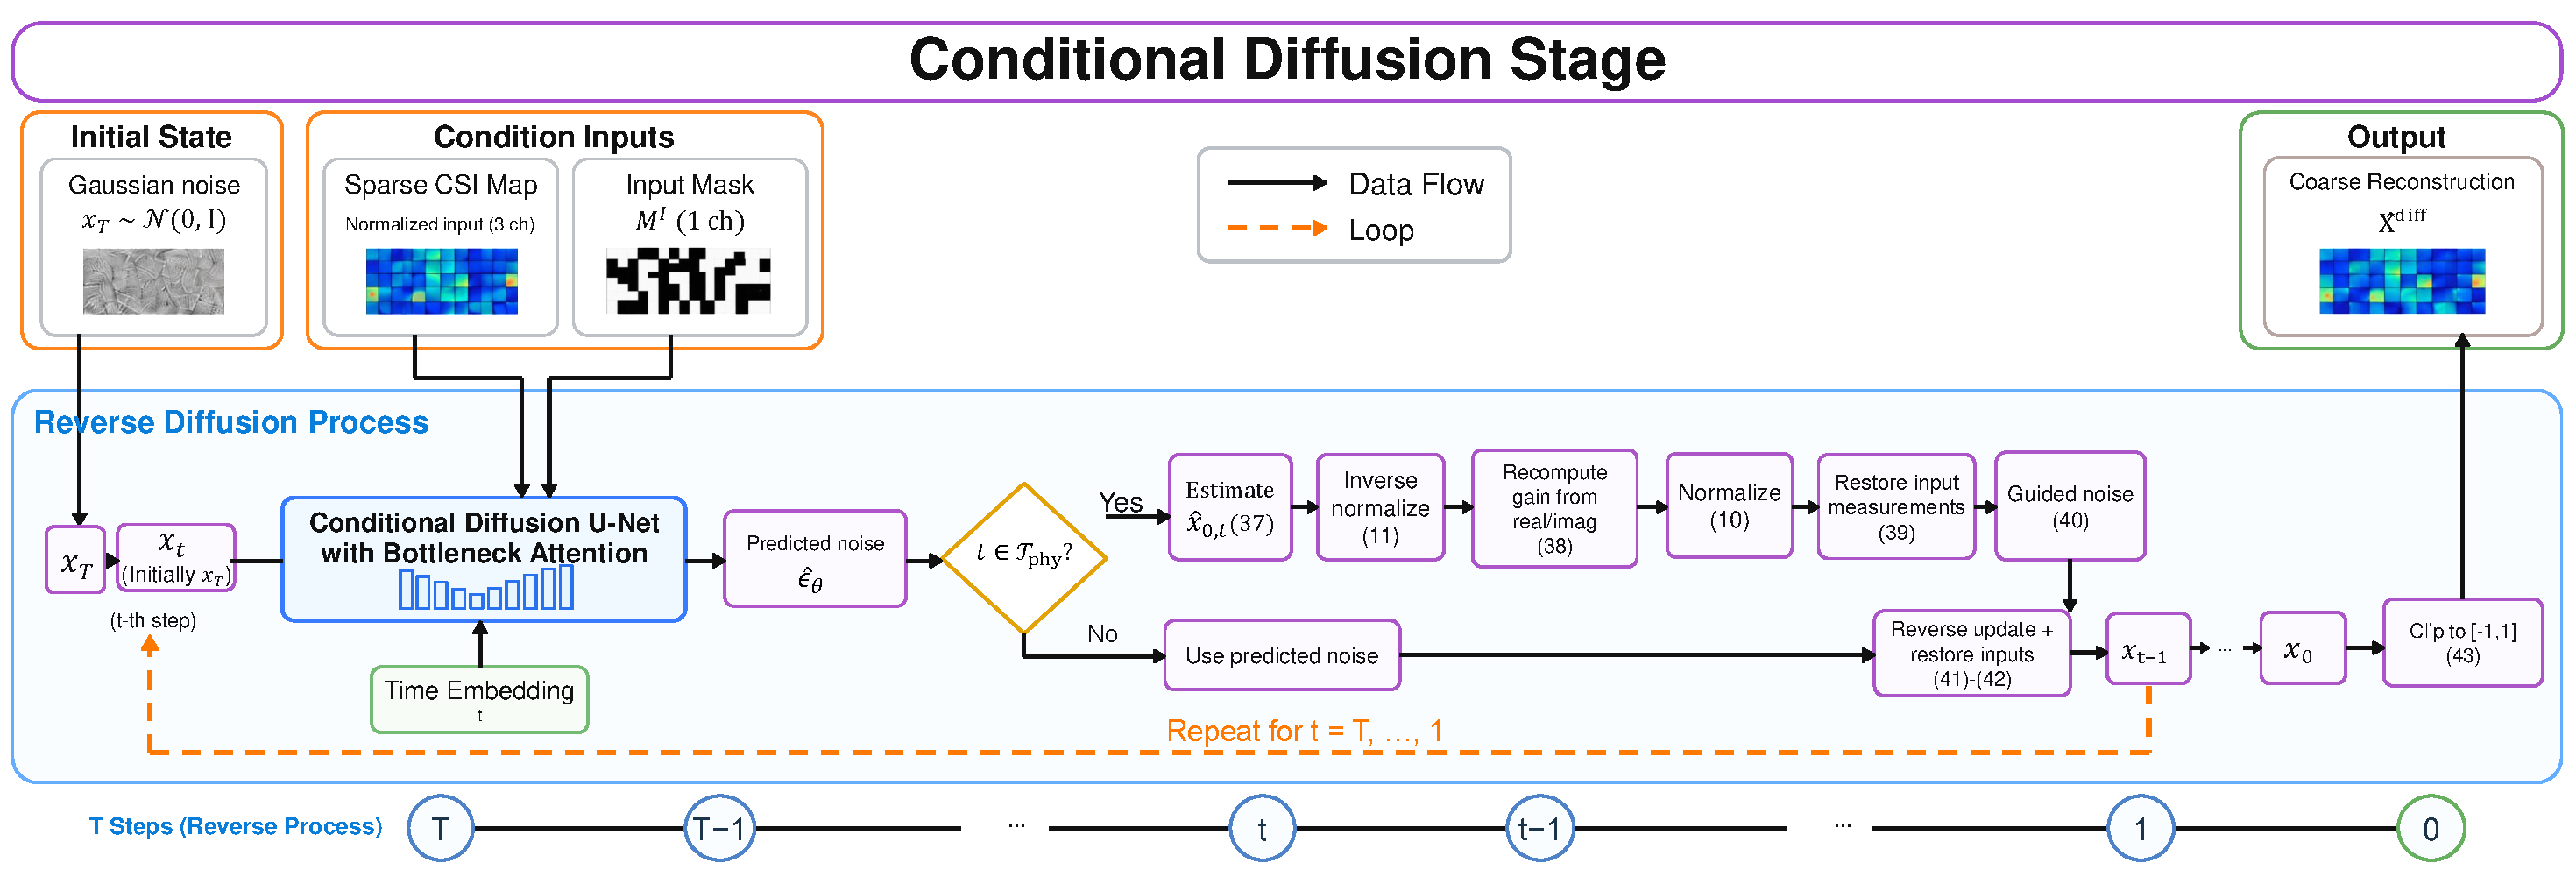
\includegraphics[width=0.98\textwidth]{figures/conditional_diffusion_stage.pdf}
	\caption{\protect\centering Inference workflow of the conditional diffusion stage.}
	\label{fig:conditional_diffusion_stage}
\end{figure*}

As shown in Fig.~\ref{fig:conditional_diffusion_stage}, inference starts from $\mat{x}_{T}\sim\mathcal{N}(\mat{0},\mat{I})$ and repeats the reverse step for $t=T,T-1,\ldots,1$. At each step, the conditional U-Net takes $\mat{x}_t$, the normalized input map $\widetilde{\mat{X}}^{I}$, the input mask $\mat{M}^{I}$, and the time index $t$ to predict noise. If $t\in\mathcal{T}_{\mathrm{phy}}$, a clean map is estimated and converted to the original scale; its amplitude channel is recomputed from the real and imaginary channels, and the corrected map is normalized again before the input measurements are restored and the noise estimate is updated. Otherwise, the original noise prediction is used. Both branches feed the reverse update that produces $\mat{x}_{t-1}$ and restores the input measurements. After the last step, $\mat{x}_0$ is clipped to give the coarse reconstruction. Here, $\beta_t$ denotes the noise variance at step $t$, $\alpha_t=1-\beta_t$, and $\bar{\alpha}_t=\prod_{s=1}^{t}\alpha_s$. In the Gaussian notation, $\mat{0}\in\mathbb{R}^{3N^2}$ is the zero mean vector and $\mat{I}\in\mathbb{R}^{3N^2\times3N^2}$ is the identity covariance matrix; sampled vectors are reshaped to tensors of size $3\times N\times N$.

\subsubsection{Conditional denoising network}

The conditional diffusion network, denoted by $\mathcal{D}_{\theta}$, predicts the injected Gaussian noise as
\begin{equation}
    \widehat{\vect{\epsilon}}_{\theta}=\mathcal{D}_{\theta}(\mat{x}_t,t,\widetilde{\mat{X}}^{I},\mat{M}^{I}).
    \label{eq:noise_prediction}
\end{equation}
The backbone is a residual U-Net with sinusoidal time embedding, two downsampling stages, a bottleneck self-attention block, and symmetric decoding with skip connections. The conditioning information is injected by concatenating the current noisy sample, the normalized input CSI map, and its mask:
\begin{align}
    \mat{U}_0
    &=\Concat\big(\mat{x}_t,\widetilde{\mat{X}}^{I},\mat{M}^{I}\big), \\
    \mat{F}_0
    &=\Conv_{3\times 3}(\mat{U}_0),
    \label{eq:diff_input_projection}
\end{align}
where $\Concat(\cdot)$ denotes concatenation along the channel dimension and $\Conv_{a\times a}(\cdot)$ denotes an $a\times a$ convolution. Thus, $\mat{U}_0\in\mathbb{R}^{7\times N\times N}$ contains the $3$ noisy channels, $3$ sparse CSI channels, and $1$ mask channel.
The diffusion index is encoded through a sinusoidal embedding followed by a learnable multilayer projection,
\begin{equation}
    \vect{e}_t=\mathrm{MLP}\!\left(
    \big[\sin(t\boldsymbol{\nu}),\cos(t\boldsymbol{\nu})\big]
    \right),
    \label{eq:time_embedding}
\end{equation}
where $\mathrm{MLP}(\cdot)$ is a learned projection with two layers and $\boldsymbol{\nu}=[\nu_0,\ldots,\nu_{m-1}]^T$ is the fixed frequency vector with
\begin{equation}
    \nu_r=\exp\!\left(-\frac{r\log(10000)}{\max(m-1,1)}\right),
    \quad r=0,\ldots,m-1,
    \label{eq:time_frequency}
\end{equation}
where $m=d_{\mathrm{emb}}/2$ and $d_{\mathrm{emb}}$ is the dimension of the time embedding. A residual block conditioned on time, as used in the encoder, bottleneck, and decoder, can then be written as
\begin{align}
    \mat{H}_1
    &=\Conv_{3\times 3}\!\left(\SiLU(\GN(\mat{F}))\right) \notag\\
    &\quad+\Linear(\SiLU(\vect{e}_t)), \\
    \mat{H}_2
    &=\Conv_{3\times 3}\!\left(\Dropout(\SiLU(\GN(\mat{H}_1)))\right), \\
    \Res(\mat{F},\vect{e}_t)
    &=\mat{H}_2+\Skip(\mat{F}),
    \label{eq:time_resblock}
\end{align}
where $\GN(\cdot)$, $\SiLU(\cdot)$, $\Linear(\cdot)$, and $\Dropout(\cdot)$ denote group normalization, SiLU activation, linear projection, and dropout, respectively. The operator $\Skip(\cdot)$ is the identity map when the channel dimensions match and a $1\times1$ convolution otherwise.

Using \eqref{eq:time_resblock}, the main network computation is summarized as
\begin{align}
    \mat{S}_1 &= \Res(\mat{F}_0,\vect{e}_t), \\
    \mat{S}_2 &= \Res(\Down(\mat{S}_1),\vect{e}_t), \\
    \mat{B}_0 &= \Res(\Down(\mat{S}_2),\vect{e}_t), \\
    \mat{B}_1 &= \Attn(\mat{B}_0), \\
    \mat{B}_2 &= \Res(\mat{B}_1,\vect{e}_t), \\
    \mat{D}_2
    &= \Res\!\left(\Concat(\Up(\mat{B}_2),\mat{S}_2),\vect{e}_t\right), \\
    \mat{D}_1
    &= \Res\!\left(\Concat(\Up(\mat{D}_2),\mat{S}_1),\vect{e}_t\right), \\
    \widehat{\vect{\epsilon}}_{\theta}
    &= \Head(\mat{D}_1).
    \label{eq:diff_unet_computation}
\end{align}
Here, $\Down(\cdot)$ is a stride-2 convolutional downsampling operator, $\Up(\cdot)$ is bilinear upsampling followed by convolutional projection, and $\mat{S}_1$ and $\mat{S}_2$ are the skip features passed from the encoder to the decoder. At the bottleneck, attention acts on the flattened spatial grid:
\begin{align}
    \mat{A}_0 &= \mathrm{reshape}(\GN(\mat{B}_0)), \\
    \mat{A}_1 &= \mat{A}_0+\mathrm{MHA}(\mat{A}_0,\mat{A}_0,\mat{A}_0), \\
    \Attn(\mat{B}_0)
    &= \mathrm{reshape}^{-1}\!\left(\mat{A}_1+\mathrm{FFN}(\mat{A}_1)\right),
    \label{eq:bottleneck_attention}
\end{align}
where $N'$ is the side length of the bottleneck feature grid, $\mathrm{reshape}(\cdot)$ converts a feature tensor of size $C\times N'\times N'$ into a sequence of $(N')^2$ feature vectors of dimension $C$, and $\mathrm{reshape}^{-1}(\cdot)$ restores the spatial arrangement. In addition, $\mathrm{MHA}(\cdot)$ denotes multi-head self-attention and $\mathrm{FFN}(\cdot)$ denotes its feedforward subnetwork. The decoder output is mapped to three noise channels by
\begin{align}
    \Head(\mat{D}_1)
    =
    \Conv_{1\times1}\!\left(
    \SiLU(\Conv_{3\times3}(\SiLU(\GN(\mat{D}_1))))
    \right).
    \label{eq:diff_output_head}
\end{align}
Fig.~\ref{fig:conditional_diffusion_unet} shows the resulting network structure. Its labels $\widetilde{\mat{Y}}$ and $\mat{M}$ denote the normalized input $\widetilde{\mat{X}}^{I}$ and input mask $\mat{M}^{I}$ used here. These inputs enter every denoising step through the seven-channel input tensor, while the time embedding is added to all residual blocks. The detailed numerical hyperparameters are reported in Table~\ref{tab:exp_hparams}.

\begin{figure*}[t]
    \centering
    \captionsetup{font=footnotesize}
    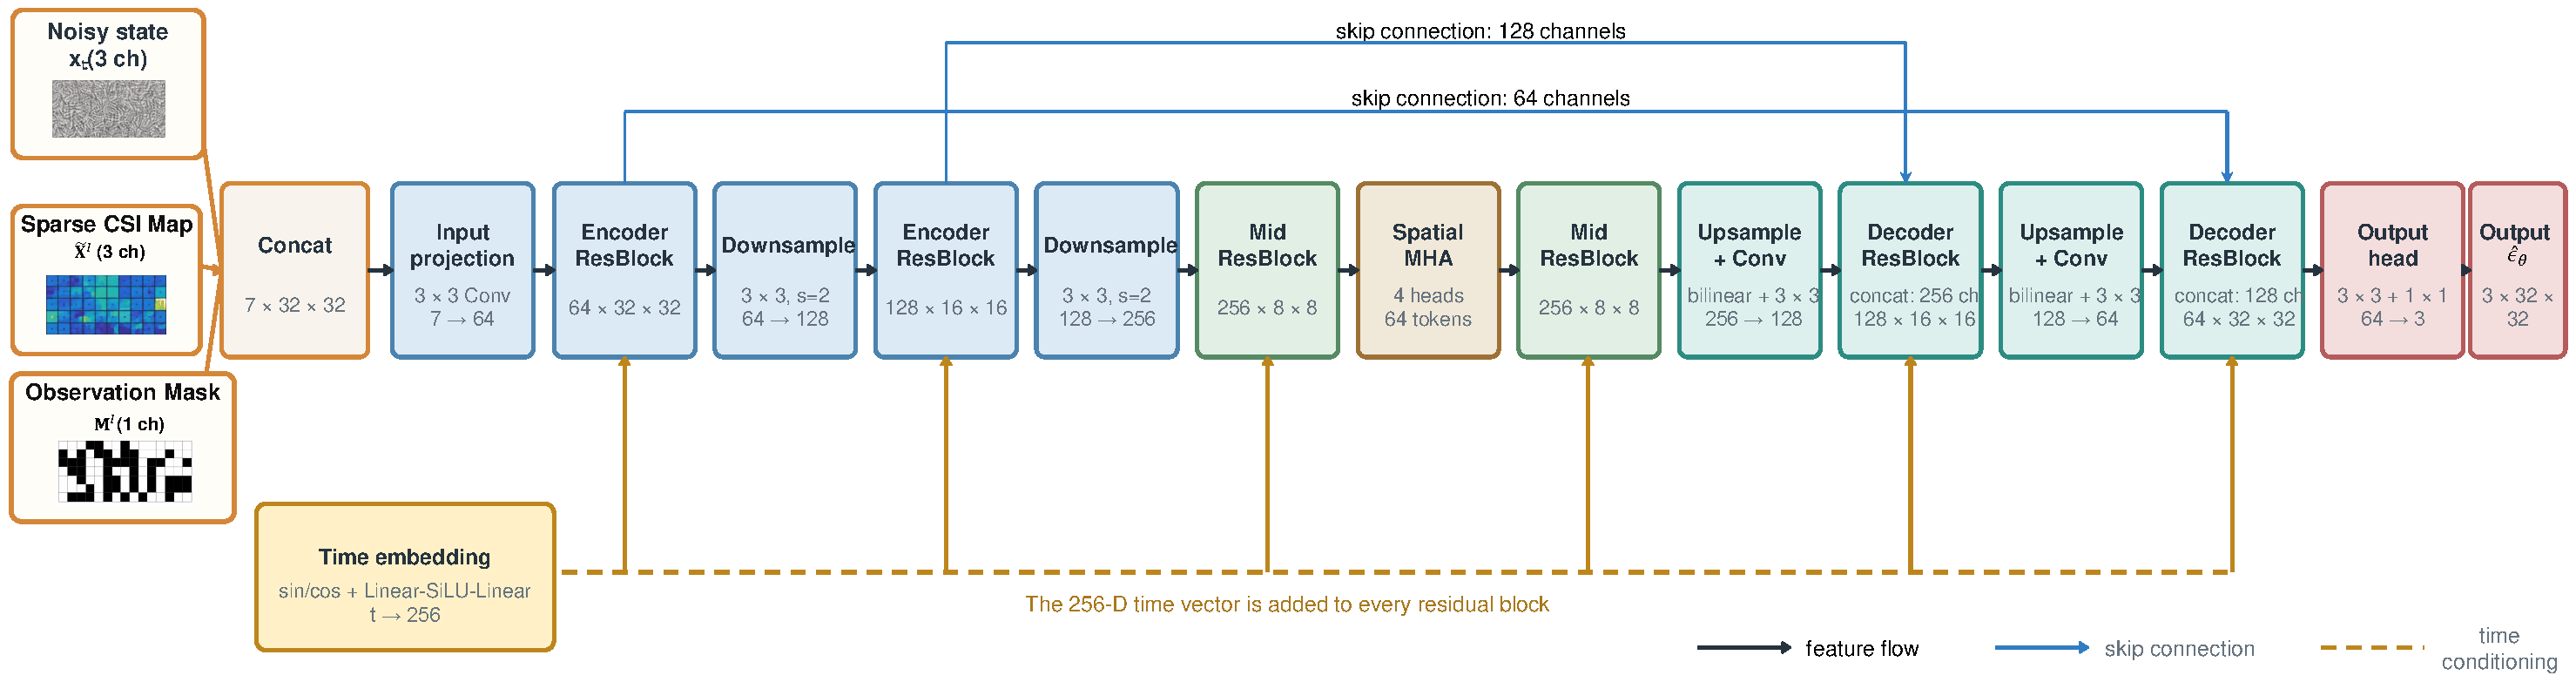
\includegraphics[width=0.98\textwidth]{figures/conditional_diffusion_unet_architecture.pdf}
    \caption{Conditional diffusion U-Net used for noise prediction at reverse step $t$.}
    \label{fig:conditional_diffusion_unet}
\end{figure*}

\subsubsection{Reverse sampling with periodic physics guidance}

The U-Net first predicts $\widehat{\vect{\epsilon}}_{\theta}$ from the current $\mat{x}_t$ by \eqref{eq:noise_prediction}. Physics guidance is applied only at selected reverse steps. Let $L_{\mathrm{phy}}\in\mathbb{N}_{+}$ be the guidance interval and define those steps by
\begin{equation}
    \mathcal{T}_{\mathrm{phy}}
    =\left\{t\in\{1,\ldots,T\}:(T-t+1)\bmod L_{\mathrm{phy}}=0\right\}.
    \label{eq:physics_guidance_steps}
\end{equation}
For $t\in\mathcal{T}_{\mathrm{phy}}$, the predicted noise gives an estimate of the clean map,
\begin{equation}
    \widehat{\mat{x}}_{0,t}=
    \operatorname{clip}_{[-1,1]}\!\left(
    \frac{\mat{x}_t-\sqrt{1-\bar{\alpha}_t}\,\widehat{\vect{\epsilon}}_{\theta}}{\sqrt{\bar{\alpha}_t}}
    \right).
    \label{eq:x0_estimate}
\end{equation}
Here, $\operatorname{clip}_{[-1,1]}(\cdot)$ denotes entrywise clipping to the interval $[-1,1]$: for a scalar $a\in\mathbb{R}$, it returns $\min\{1,\max\{-1,a\}\}$. The clipping keeps the intermediate clean estimate within the normalized data range. The estimate is then converted to the original scale by \eqref{eq:inverse_normalization}, giving $\widehat{\mat{X}}^{\mathrm{phys}}_{0,t}=\big[\widehat{\mat{X}}^{\mathrm g}_{0,t},\widehat{\mat{X}}^{\mathrm{re}}_{0,t},\widehat{\mat{X}}^{\mathrm{im}}_{0,t}\big]$.

The next operation in the guided branch recomputes the amplitude channel from the real and imaginary channels at each grid location $(u,v)$:
\begin{equation}
    \widehat{X}^{\mathrm g}_{0,t}(u,v)=10\log_{10}\!\left(\sqrt{\big(\widehat{X}^{\mathrm{re}}_{0,t}(u,v)\big)^2+\big(\widehat{X}^{\mathrm{im}}_{0,t}(u,v)\big)^2}\right),
    \label{eq:physics_projection}
\end{equation}
where $\widehat{X}^{\mathrm{re}}_{0,t}(u,v)$ and $\widehat{X}^{\mathrm{im}}_{0,t}(u,v)$ are the components after inverse normalization. The corrected three-channel tensor is mapped back to normalized space by \eqref{eq:normalization}, yielding $\widehat{\mat{x}}^{\mathrm{phy}}_{0,t}$. To restore measured entries, define the observation consistency operator
\begin{equation}
	\Pi_{\mathrm{obs}}(\mat{Z})=(\mat{1}-\mat{M}^{I})\od\mat{Z}+\mat{M}^{I}\od\widetilde{\mat{X}}^{I},
	\label{eq:obs_projection}
\end{equation}
where $\mat{Z}\in\mathbb{R}^{3\times N\times N}$ is any normalized intermediate map and $\mat{1}\in\R^{N\times N}$ is the matrix of ones. Both $\mat{1}$ and $\mat{M}^{I}$ are broadcast across the three channel components. The operator retains estimated values outside the input mask and replaces input entries with their measurements. Applying it to the corrected clean estimate gives the noise used for the reverse update:
\begin{equation}
    \widetilde{\vect{\epsilon}}_{\theta}
    =
    \frac{\mat{x}_t-\sqrt{\bar{\alpha}_t}\,
    \Pi_{\mathrm{obs}}(\widehat{\mat{x}}^{\mathrm{phy}}_{0,t})}
    {\sqrt{1-\bar{\alpha}_t}},
    \label{eq:guided_noise_update}
\end{equation}
When $t\notin\mathcal{T}_{\mathrm{phy}}$, the clean estimate and amplitude correction are skipped, and $\widetilde{\vect{\epsilon}}_{\theta}=\widehat{\vect{\epsilon}}_{\theta}$. The experiments use $L_{\mathrm{phy}}=25$, as reported in Table~\ref{tab:exp_hparams}.

Using the guided noise estimate, or the original prediction when guidance is skipped, the reverse mean and state update are
\begin{align}
    \boldsymbol{\mu}_{\theta}(\mat{x}_t,t)
    &=
    \frac{1}{\sqrt{\alpha_t}}
    \left(
    \mat{x}_t-
    \frac{\beta_t}{\sqrt{1-\bar{\alpha}_t}}\widetilde{\vect{\epsilon}}_{\theta}
    \right),
    \label{eq:reverse_mean} \\
    \mat{x}_{t-1}
    &=
    \Pi_{\mathrm{obs}}\!\left(
    \boldsymbol{\mu}_{\theta}(\mat{x}_t,t)+\sigma_t\vect{z}
    \right),
    \label{eq:reverse_update}
\end{align}
where $\sigma_t=\sqrt{\beta_t}$ is the standard deviation of the sampling noise, with $\vect{z}\sim\mathcal{N}(\mat{0},\mat{I})$ for $t>1$ and $\vect{z}=\mat{0}$ at the final reverse step. The operator $\Pi_{\mathrm{obs}}$ restores measurements after every update. The resulting $\mat{x}_{t-1}$ becomes the input to the U-Net at the next time step, so the prediction, optional guidance, and reverse update repeat until $\mat{x}_0$ is obtained.

After the final step, the coarse diffusion output is clipped to the normalized range and denoted by
\begin{equation}
    \widehat{\mat{X}}^{\mathrm{diff}}
    =\operatorname{clip}_{[-1,1]}(\mat{x}_0)
    =\mathcal{G}_{\theta}(\widetilde{\mat{X}}^{I},\mat{M}^{I}).
    \label{eq:coarse_output}
\end{equation}

\subsubsection{Diffusion training objective}

For fully supervised training, let $\widetilde{\mat{X}}$ be a normalized map obtained from a fully measured sample $\mat{X}_s$ with $\mathcal{A}_s=\Omega$. A time index $t\in\{1,\ldots,T\}$ is sampled, and the forward noising process produces
\begin{equation}
    \mat{x}_t=\sqrt{\bar{\alpha}_t}\,\widetilde{\mat{X}}+\sqrt{1-\bar{\alpha}_t}\,\vect{\epsilon},
    \qquad
    \vect{\epsilon}\sim\mathcal{N}(\mat{0},\mat{I}),
    \label{eq:forward_diffusion}
\end{equation}
where $\vect{\epsilon}$ is reshaped to a tensor of size $3\times N\times N$. The denoising network predicts this injected noise from $\mat{x}_t$, $t$, $\widetilde{\mat{X}}^{I}$, and $\mat{M}^{I}$ by \eqref{eq:noise_prediction}. To emphasize reconstruction of positions omitted from the model input, the noise prediction loss is spatially weighted. Define
\begin{equation}
    \omega(u,v)=M^{I}(u,v)+\lambda_{\mathrm{miss}}\big(1-M^{I}(u,v)\big),
    \label{eq:weight_function}
\end{equation}
where $\lambda_{\mathrm{miss}}>1$ is the missing region weight. The diffusion loss is then
\begin{equation}
    \mathcal{L}_{\mathrm{diff}}=
    \frac{1}{3N^2}
    \sum_{c=1}^{3}\sum_{(u,v)\in\Omega}
    \omega(u,v)\big(\widehat{\epsilon}_{\theta,c}(u,v)-\epsilon_c(u,v)\big)^2.
    \label{eq:diffusion_loss}
\end{equation}
This objective follows standard denoising diffusion probabilistic learning and trains the model in noise space rather than directly in CSI space. The physics projection and restoration of measured values are used during sampling and are not included in the diffusion training loss.

\subsection{Physics Informed Refinement Stage}

\subsubsection{Refinement Network interpretation}

Fig.~\ref{fig:pinn_refiner_arch} details the refinement stage. The upper branch uses a trainable propagation center, path loss exponent, and wave number to compute one amplitude map and two phase maps. The lower branch concatenates these maps with the diffusion estimate, input mask, and coordinate tensor, and processes the resulting tensor with a compact encoder and decoder. Thus, \emph{physics informed refinement} here refers to the explicit use of coordinate and propagation features in the learned correction; it does not impose an exact propagation equation on the output.

\begin{figure*}[t]
    \centering
    \captionsetup{font=footnotesize}
    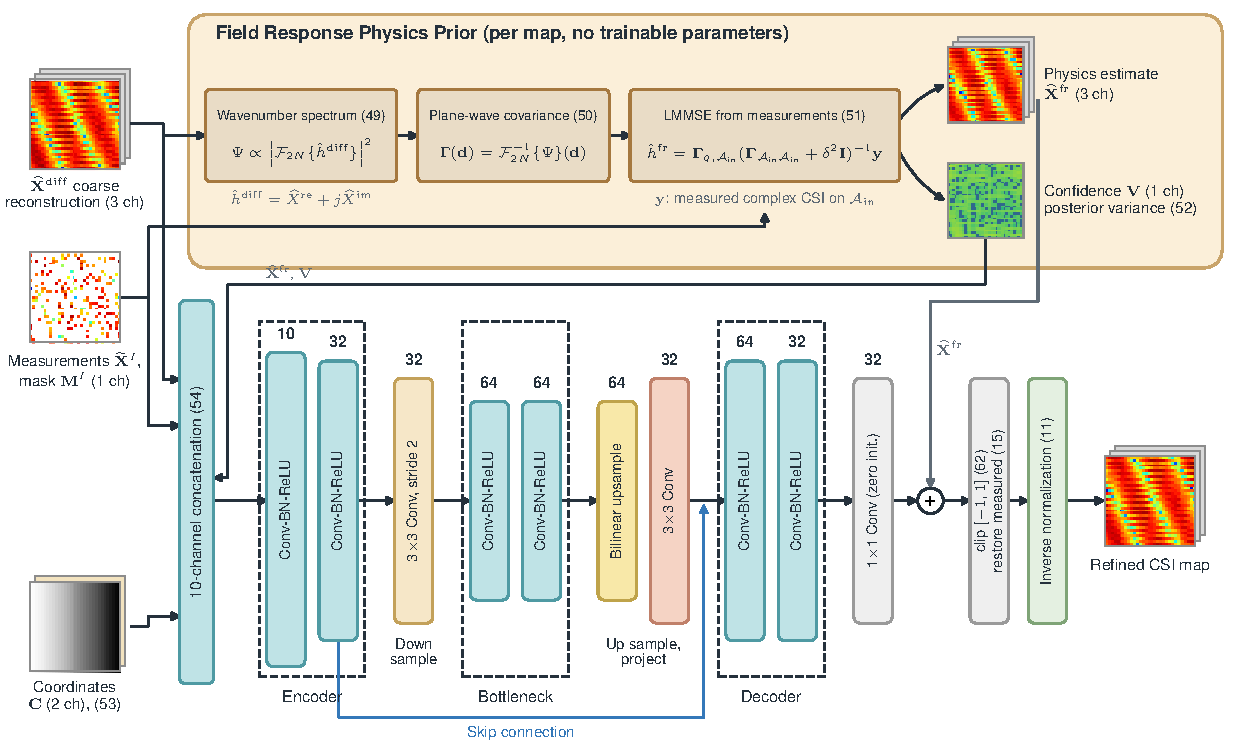
\includegraphics[width=0.92\textwidth]{figures/pinn_refiner_architecture.pdf}
    \caption{\protect\centering Architecture of the PINN refiner in PIDR-Net.}
    \label{fig:pinn_refiner_arch}
\end{figure*}


\subsubsection{Learnable propagation prior}

The propagation branch forms approximate radial attenuation and phase patterns from a few trainable scalars in $\phi$ shared across samples. These internal features do not represent the actual geometry between the transmitter and receiver or determine the reconstructed channel by themselves.

Let the normalized coordinate tensor on the discrete spatial grid be denoted by
\begin{equation}
	\mat{C}(u,v)=\big[x(u,v),y(u,v)\big]^T,
	\qquad (u,v)\in\Omega,
	\label{eq:coordinate_tensor}
\end{equation}
where $\Omega=\{1,\ldots,N\}\times\{1,\ldots,N\}$ is the set of all grid indices, and $x(u,v),y(u,v)\in[0,1]$ are the normalized horizontal and vertical coordinates of grid location $(u,v)$, respectively. Equivalently, the full coordinate tensor satisfies $\mat{C}\in\mathbb{R}^{2\times N\times N}$, where the first channel stores the $x$-coordinates and the second channel stores the $y$-coordinates. The same coordinate tensor is used for all samples with the same spatial resolution.
In this work, the coordinate normalization is
\begin{equation}
	x(u,v)=\frac{v-1}{N-1},
	\qquad
	y(u,v)=\frac{u-1}{N-1},
	\label{eq:coordinate_normalization}
\end{equation}
Thus, $\mat{C}$ depends only on grid resolution and tells the refiner each feature's location, which the diffusion estimate and input mask do not encode explicitly.

The prior branch first introduces a learnable propagation center in the normalized coordinate system,
\begin{equation}
	x_{\mathrm{pc}}=\sigma(\xi_x),
	\qquad
	y_{\mathrm{pc}}=\sigma(\xi_y),
	\label{eq:propagation_center}
\end{equation}
where $\xi_x$ and $\xi_y$ are unconstrained learnable raw parameters and $\sigma(\cdot)$ is the sigmoid function. The sigmoid mapping confines $x_{\mathrm{pc}}$ and $y_{\mathrm{pc}}$ to the interval $[0,1]$, so that the learned propagation center remains inside the normalized reconstruction region. This center is a trainable spatial reference point used to construct radial prior features, rather than a known physical transmitter or receiver coordinate.

Given this learned center, the branch computes the Euclidean distance from the propagation center to each candidate MA grid point,
\begin{equation}
	d(u,v)=\sqrt{\big(x(u,v)-x_{\mathrm{pc}}\big)^2+\big(y(u,v)-y_{\mathrm{pc}}\big)^2},
	\label{eq:distance_map}
\end{equation}
where $d(u,v)$ is the distance map. This distance is not assumed to be the true separation between the transmitter and receiver; instead, it is the geometric variable used to construct the radial priors for amplitude and phase.

The other two physical quantities are a learnable path loss exponent and a learnable wave number, defined as
\begin{equation}
	n=\softplus(\xi_n)+1,
	\qquad
	k=\softplus(\xi_k)+10^{-3},
	\label{eq:nk_parameters}
\end{equation}
where $\xi_n$ and $\xi_k$ are unconstrained learnable raw parameters. The $\softplus(\cdot)$ mapping guarantees positivity, while the constants $1$ and $10^{-3}$ further prevent degenerate values during training. Here, $n$ controls how the prior attenuation changes with distance, whereas $k$ controls the spatial oscillation frequency of the phase prior.

Based on $d(u,v)$, $n$, and $k$, the prior feature maps are constructed as
\begin{align}
	\mat{A}_{\mathrm{pr}}(u,v)
	&=a_s\big[-10n\log_{10}(d(u,v)+10^{-3})\big]+a_b,
	\label{eq:amp_prior}\\
	\mat{R}_{\mathrm{pr}}(u,v)
	&=\cos\big(kd(u,v)+\varphi_b\big),
	\label{eq:re_prior}\\
	\mat{I}_{\mathrm{pr}}(u,v)
	&=\sin\big(kd(u,v)+\varphi_b\big),
	\label{eq:im_prior}
\end{align}
where $\mat{A}_{\mathrm{pr}}(u,v)$ is the amplitude prior, $\mat{R}_{\mathrm{pr}}(u,v)$ is the phase real prior, and $\mat{I}_{\mathrm{pr}}(u,v)$ is the phase imaginary prior. In addition, $a_s$ and $a_b$ are learnable scale and bias terms for the amplitude branch, and $\varphi_b$ is a learnable phase offset. Equation~\eqref{eq:amp_prior} describes an approximate logarithmic attenuation trend. Equations~\eqref{eq:re_prior} and \eqref{eq:im_prior} describe the real and imaginary parts of a radial sinusoidal pattern.

Finally, the three prior maps are concatenated along the channel dimension to form the propagation prior tensor,
\begin{equation}
	\mat{P}_{\mathrm{pr}}=\big[\mat{A}_{\mathrm{pr}},\mat{R}_{\mathrm{pr}},\mat{I}_{\mathrm{pr}}\big]\in\mathbb{R}^{3\times N\times N}.
	\label{eq:prior_tensor}
\end{equation}
The refiner combines $\mat{P}_{\mathrm{pr}}$ with the diffusion estimate, mask, and $\mat{C}$. Coordinates identify grid positions; the prior offers learned radial attenuation and phase patterns for correcting unobserved entries, without imposing an exact propagation law.

\subsubsection{Input features and network structure}

Within the PINN refiner, the coarse diffusion reconstruction and input mask are concatenated with the internally constructed propagation prior and coordinate tensor:
\begin{equation}
    \mat{Z}_{\mathrm{in}}=\Concat\big(\widehat{\mat{X}}^{\mathrm{diff}},\mat{M}^{I},\mat{P}_{\mathrm{pr}},\mat{C}\big).
    \label{eq:pinn_input_tensor}
\end{equation}
Hence, the effective input dimensionality is nine channels. The refinement backbone can be written compactly as
\begin{equation}
    \widehat{\mat{X}}^{\mathrm{pinn}}
    =\tanh\!\left(\mathcal{B}_{\phi}(\mat{Z}_{\mathrm{in}})\right),
    \label{eq:pinn_backbone_map}
\end{equation}
where $\mathcal{B}_{\phi}$ denotes the encoder and decoder before the final bounded activation. The output is the normalized refined map. The network uses two convolutional blocks at the input resolution, one stride 2 downsampling layer, a bottleneck block, bilinear upsampling, skip fusion, and a final $\tanh$ output layer.

The refinement network contains the propagation branch in \eqref{eq:prior_tensor} and a convolutional reconstruction network. The propagation branch produces the three auxiliary maps defined above. The basic convolutional unit is
\begin{equation}
    \CBR_{\ell}(\mat{F})
    =
    \ReLU\!\left(\BN\!\left(\Conv_{3\times3}^{(\ell)}(\mat{F})\right)\right),
    \label{eq:cbr_block}
\end{equation}
where $\CBR_{\ell}(\cdot)$ denotes Conv-BN-ReLU block $\ell$, $\BN(\cdot)$ denotes batch normalization, and $\ReLU(\cdot)$ denotes the rectified linear unit activation. The encoder at the original resolution extracts shallow spatial features through two such blocks:
\begin{equation}
    \mat{E}
    =
    \Enc(\mat{Z}_{\mathrm{in}})
    =
    \CBR_{2}\!\left(\CBR_{1}(\mat{Z}_{\mathrm{in}})\right).
    \label{eq:pinn_encoder}
\end{equation}
The downsampling and bottleneck operations are then
\begin{align}
    \mat{G}
    &=\Conv_{3\times3,s=2}(\mat{E}), \\
    \mat{B}
    &=\CBR_{4}\!\left(\CBR_{3}(\mat{G})\right),
    \label{eq:pinn_down_bottleneck}
\end{align}
where the stride-2 convolution reduces the spatial resolution and increases the channel width, allowing the bottleneck to aggregate a larger local context.

The decoder first upsamples the bottleneck features back to the encoder resolution, projects them by convolution, and fuses them with the encoder skip feature:
\begin{align}
    \mat{U}
    &=\Conv_{3\times3}\!\left(\Interp(\mat{B})\right), \\
    \mat{D}
    &=\Dec\!\left(\Concat(\mat{U},\mat{E})\right) \notag\\
    &=\CBR_{6}\!\left(\CBR_{5}\!\left(\Concat(\mat{U},\mat{E})\right)\right).
    \label{eq:pinn_decoder}
\end{align}
Here, $\Interp(\cdot)$ denotes bilinear interpolation that resizes the bottleneck feature map to the spatial resolution of the encoder feature $\mat{E}$ before skip fusion.
Finally, a $1\times1$ projection maps the decoded feature back to the three CSI channels, and the bounded activation keeps the prediction in the normalized range:
\begin{equation}
    \widehat{\mat{X}}^{\mathrm{pinn}}
    =
    \tanh\!\left(\Conv_{1\times1}(\mat{D})\right).
    \label{eq:pinn_output}
\end{equation}
Equations~\eqref{eq:pinn_input_tensor}--\eqref{eq:pinn_output} show explicitly how the diffusion reconstruction, input mask, learnable propagation prior, and coordinate tensor are fused before spatial refinement. The detailed channel width used in the experiments is reported in Table~\ref{tab:exp_hparams}.

The refinement network is smaller than the diffusion network because it operates on an already completed map. Its convolutional layers correct local errors and spatial transitions, while the prior and coordinate channels provide the corresponding grid information. The diffusion and refinement stages therefore perform map completion and correction, respectively.

\subsubsection{Refinement objective}

The refinement stage is trained in normalized space with a missing region reconstruction objective:
\begin{equation}
    \mathcal{L}_{\mathrm{data}}=
    \frac{\norm{(\mat{1}-\mat{M}^{I})\od(\widehat{\mat{X}}^{\mathrm{pinn}}-\widetilde{\mat{X}}^{L})}_{1}}
    {\sum_{(u,v)\in\Omega}(1-M^{I}(u,v))}.
    \label{eq:data_loss}
\end{equation}
For fully measured training maps, $\mat{M}^{L}$ covers the full grid, so this term evaluates the refiner at positions withheld from the model input. After refinement, the input entries are reinserted according to \eqref{eq:final_estimator}, so the final PIDR-Net output preserves the supplied CSI values exactly. The diffusion and refinement stages use the separate objectives in \eqref{eq:diffusion_loss} and \eqref{eq:data_loss}; physical information enters through the sampling projection, propagation prior, coordinates, and restoration of measured values.

\subsection{Training and Inference Algorithms}

The complete workflow is summarized by Algorithms~\ref{alg:offline_training} and~\ref{alg:online_inference}.

\begin{algorithm}[t]
\caption{Offline Training of the Two PIDR-Net Stages}
\label{alg:offline_training}
\begin{algorithmic}[1]
\STATE Organize each fully measured sample $\mat{X}_s$ as aligned amplitude, real, and imaginary maps.
\STATE Split the offline samples into training and evaluation sets, and select the input positions $\mathcal{A}_{s,\mathrm{in}}$ by random masking.
\STATE Compute the channel extrema from these input positions by \eqref{eq:normalization_extrema}; normalize $\mat{X}_s$ and form $(\widetilde{\mat{X}},\widetilde{\mat{X}}^{I},\mat{M}^{I},\mat{M}^{L})$, with $\mat{M}^{L}=\mat{1}$.
\FOR{each diffusion epoch}
    \STATE Sample $t\in\{1,\ldots,T\}$ and $\vect{\epsilon}\sim\mathcal{N}(\mat{0},\mat{I})$, synthesize $\mat{x}_t$ by \eqref{eq:forward_diffusion}, and predict the noise by \eqref{eq:noise_prediction}.
    \STATE Update $\theta$ using the spatially weighted noise prediction loss in \eqref{eq:diffusion_loss}.
\ENDFOR
\STATE Freeze the trained diffusion model.
\STATE Generate coarse reconstructions with physics guidance by iterating \eqref{eq:noise_prediction}, \eqref{eq:guided_noise_update}, and \eqref{eq:reverse_update}.
\STATE Store the diffusion reconstructions to avoid repeated sampling during refiner training.
\FOR{each PINN epoch}
    \STATE Refine the cached diffusion output using the mask, propagation prior, and coordinate features.
    \STATE Update $\phi$ using the $\ell_1$ loss over the missing region in \eqref{eq:data_loss}.
\ENDFOR
\end{algorithmic}
\end{algorithm}

\begin{algorithm}[t]
\caption{Online Sparse CSI Map Reconstruction}
\label{alg:online_inference}
\begin{algorithmic}[1]
\REQUIRE Normalized input CSI map $\widetilde{\mat{X}}^{I}$, input mask $\mat{M}^{I}$, trained parameters $\theta$ and $\phi$
\ENSURE Reconstructed normalized CSI map $\widehat{\mat{X}}_{\mathrm n}$
\STATE Initialize $\mat{x}_{T}\sim\mathcal{N}(\mat{0},\mat{I})$.
\FOR{$t=T,T-1,\ldots,1$}
    \STATE Predict noise $\widehat{\vect{\epsilon}}_{\theta}=\mathcal{D}_{\theta}(\mat{x}_t,t,\widetilde{\mat{X}}^{I},\mat{M}^{I})$.
    \IF{$t\in\mathcal{T}_{\mathrm{phy}}$ as defined in \eqref{eq:physics_guidance_steps}}
        \STATE Recover the clean estimate $\widehat{\mat{x}}_{0,t}$ using \eqref{eq:x0_estimate} and recompute its gain channel using \eqref{eq:physics_projection}.
        \STATE Apply \eqref{eq:obs_projection} to the corrected clean estimate and recompute $\widetilde{\vect{\epsilon}}_{\theta}$ using \eqref{eq:guided_noise_update}.
    \ELSE
        \STATE Set $\widetilde{\vect{\epsilon}}_{\theta}\leftarrow\widehat{\vect{\epsilon}}_{\theta}$.
    \ENDIF
    \STATE Obtain $\mat{x}_{t-1}$ using \eqref{eq:reverse_update}, which includes restoration of the measured values.
\ENDFOR
\STATE Set $\widehat{\mat{X}}^{\mathrm{diff}}\leftarrow\operatorname{clip}_{[-1,1]}(\mat{x}_0)$ and refine it using \eqref{eq:pinn_stage}.
\STATE Reinsert the observed entries using \eqref{eq:final_estimator} to obtain $\widehat{\mat{X}}_{\mathrm n}$.
\STATE If required, obtain the estimate $\widehat{\mat{X}}$ on the original scale using \eqref{eq:inverse_normalization} channel by channel.
\STATE \textbf{return} $\widehat{\mat{X}}_{\mathrm n}$ and, when requested, $\widehat{\mat{X}}$.
\end{algorithmic}
\end{algorithm}

\subsubsection{Semi-supervised training under partial offline measurements}

The default protocol above assumes that complete CSI maps are available during offline training, so sparse inputs can be simulated by masking fully measured maps. In practical MA deployment, however, exhaustive offline sounding over all candidate positions may itself be expensive. To model this situation, PIDR-Net can also use semi-supervised training, in which each training map contains only a subset of actually sounded grid points.

Let the total available ratio be $\alpha\in(0,1]$, meaning that a fraction $\alpha$ of the full grid positions is sounded for each training sample. For sample $s$, this is the available set $\mathcal{A}_s$ defined in Section~\ref{sec:offline_measurements}. A fraction $\zeta$ of $\mathcal{A}_s$ is assigned to the input set $\mathcal{A}_{s,\mathrm{in}}$ defined above, while the remaining set $\mathcal{A}_{s,\mathrm{sup}}=\mathcal{A}_s\setminus\mathcal{A}_{s,\mathrm{in}}$ provides supervision labels. Here $M_s^{L}(u,v)=1$ exactly when $(u,v)\in\mathcal{A}_{s,\mathrm{sup}}$, and $\mat{X}_s^{L}=\mat{X}_s\od\mat{M}_s^{L}$. Omitting the sample index in the following losses, $\mat{M}^{I}$ conditions the model and restores its input measurements, whereas $\mat{M}^{L}$ selects measured supervision positions. Their supports are disjoint in this partial-data setting, and positions outside $\mathcal{A}_s$ are excluded from both masks.

The diffusion stage is trained with a masked noise prediction loss restricted to the supervision region. Let $N_L=\sum_{(u,v)\in\Omega}M^{L}(u,v)$ denote the number of supervision points:
\begin{equation}
	\begin{aligned}
	\mathcal{L}_{\mathrm{diff}}^{\mathrm{partial}}
	&= \frac{1}{3N_L}
	\sum_{c=1}^{3}\sum_{(u,v)\in\Omega}
	M^{L}(u,v) \\
	&\quad \times
	\big(\widehat{\epsilon}_{\theta,c}(u,v)-\epsilon_c(u,v)\big)^2.
	\end{aligned}
	\label{eq:loss_diff_partial}
\end{equation}
The refinement stage is trained with an $\ell_1$ reconstruction loss on the same supervision mask:
\begin{equation}
	\begin{aligned}
	\mathcal{L}_{\mathrm{ref}}^{\mathrm{partial}}
	&=
	\frac{
		\norm{
		\mat{M}^{L}\od
		(\widehat{\mat{X}}^{\mathrm{pinn}}-\widetilde{\mat{X}}^{L})
		}_1
	}
	{N_L}.
	\end{aligned}
	\label{eq:loss_ref_partial}
\end{equation}
All other components, including the network architectures, reverse sampling procedure, physics projection, and restoration of measured values, remain identical to those used with fully supervised PIDR-Net. Thus, semi-supervised training changes only the offline training masks and the regions on which the losses are evaluated, rather than introducing a separate reconstruction model.

\section{Experimental Results}
\label{sec:exp}

This section reports six experiments: reconstruction on the main ray tracing dataset, comparison on two additional datasets, tests with different sampling geometries and online measurement ratios, training with different offline measurement ratios, and MA position optimization. The main dataset is generated with Sionna RT; the other two are obtained from field response and electromagnetic (EM) simulations.

\subsection{Datasets and Data Preparation}

\subsubsection{Sionna RT dataset generation}
The main dataset is generated offline using Sionna RT~\cite{ref_sionna_rt}. In the adopted setup, each receiver (RX) realization corresponds to one CSI map sample. To obtain the position dependent response needed for this map, one transmit MA is scanned over a fixed 2D plane discretized into an $N\times N$ grid. For every grid point, the ray tracing simulator computes a narrowband complex channel coefficient between the current transmit antenna position and the RX realization. Its real part, imaginary part, and gain are then recorded as the three aligned channels of the CSI map. The reported setup uses a $32\times 32$ scanning grid on a fixed coordinate plane and a carrier frequency of $5$~GHz. The ray tracing configuration enables deterministic propagation mechanisms including a direct line of sight (LoS), specular reflection, refraction, and diffraction, so the generated maps reflect both direct paths and multipath effects determined by the environment.

\subsubsection{Additional datasets}
Besides the dataset generated by RT, we also conduct experiments on a field response dataset and an EM simulation dataset. These two auxiliary datasets are used to assess whether PIDR-Net remains effective when the underlying propagation statistics differ from those of the primary RT benchmark. For fairness, all three datasets are converted into the same representation with three channels, namely gain, real part, and imaginary part, and are organized on a regular spatial grid before being fed into the reconstruction network: the RT and field response datasets each contain $10000$ maps on a $32\times 32$ grid, and the EM simulation dataset contains $961$ maps on a $21\times 41$ grid. Unless otherwise stated, a separate model is trained and evaluated on each dataset; the comparison across datasets in this paper refers to applying the same reconstruction pipeline and hyperparameter protocol to datasets with different propagation statistics, rather than testing one model trained on a single dataset across all datasets.

\subsection{Benchmark Settings and Evaluation Metrics}

\subsubsection{Compared methods}
Three reconstruction strategies based on learning are compared.
\begin{itemize}
    \item \textit{Diffusion}: the conditional diffusion model alone, using physics informed reverse sampling and exact restoration of measured values;
    \item \textit{PINN}: the physics informed reconstruction network operating directly on the sparse input map and mask;
    \item \textit{PIDR-Net}: the proposed method, in which the diffusion model first produces a coarse completion and the physics informed refinement network subsequently improves local accuracy and consistency among channels.
\end{itemize}
For the sampling strategy study, three classical interpolation baselines, namely nearest neighbor, linear, and cubic interpolation, are additionally included to quantify the benefit of learned priors under irregular observation geometries.

\subsubsection{Masking protocol and evaluation settings}
Unless otherwise specified, the missing ratio is set to $0.8$, meaning that only $20\%$ of the CSI entries are observed. The observation masks are generated with a deterministic evaluation seed so that all compared methods are tested under identical sparsity patterns. For computationally intensive diffusion sampling, evaluation is performed on a fixed subset of at most $50$ test maps. The same subset and masks are used for all compared methods. Since the diffusion sampler enforces observation consistency during reverse sampling, the same restoration of measured values is also applied to the outputs of the refiner before metric calculation.

Table~\ref{tab:exp_hparams} summarizes the main hyperparameters used throughout training and evaluation. These settings are kept fixed across the principal experiments unless otherwise stated. In particular, the same masking ratio, diffusion schedule, and network widths are reused across datasets, and only the grid size and the number of training maps follow each dataset, so that the comparison emphasizes the behavior of the reconstruction methods rather than per dataset hyperparameter tuning.

\begin{table}[t]
\caption{Main experimental hyperparameters used in training and evaluation.}
\label{tab:exp_hparams}
\centering
\small
\begin{tabular}{p{0.56\columnwidth}p{0.30\columnwidth}}
\toprule
Item & Value \\ 
\midrule
Spatial resolution & $32\times 32$ ($21\times 41$ for EM) \\ 
CSI channels & $3$ (gain, real, imaginary) \\ 
Train/test split & $0.9/0.1$ \\ 
Training samples & $9000$ ($864$ for EM) \\ 
Batch size & $32$ \\ 
Optimizer & AdamW \\ 
Learning rate & $2\times 10^{-4}$ \\ 
Number of epochs & $1000$ \\ 
Diffusion steps $T$ & $1000$ \\ 
Noise schedule & cosine \\ 
Missing ratio & $0.80$ \\ 
Missing region weight $\lambda_{\mathrm{miss}}$ & $3.0$ \\ 
Physics guidance interval $L_{\mathrm{phy}}$ & every $25$ reverse steps \\ 
Diffusion base channels & $64$ \\ 
Time embedding dimension & $256$ \\ 
Diffusion dropout & $0.10$ \\ 
Attention heads & $4$ \\ 
PINN base channels & $32$ \\ 
Evaluation mask seed & $0$ \\ 
Representative evaluation samples & up to $50$ \\ 
\bottomrule
\end{tabular}
\end{table}

\subsubsection{Performance metrics}
We report four reconstruction metrics on the gain channel. For compact notation, let $G=X^{\mathrm g}$ and $\widehat{G}=\widehat{X}^{\mathrm g}$.
\begingroup
\small
\begin{align}
	\mathrm{MSE}
	&= \frac{1}{N^2}\sum_{u=1}^{N}\sum_{v=1}^{N}
	\big(G(u,v)-\widehat{G}(u,v)\big)^2, \\
	\mathrm{NMSE}_{\mathrm{dB}}
	&= 10\log_{10}\!\left(
	\frac{\mathrm{MSE}}
	{\frac{1}{N^2}\sum_{u=1}^{N}\sum_{v=1}^{N} G^2(u,v)+10^{-10}}
	\right), \\
	\mathrm{PSNR}
	&= 10\log_{10}\!\left(\frac{\mathrm{DR}^2}{\mathrm{MSE}}\right), 
	\qquad \mathrm{DR}=G_{\max}-G_{\min}, \\
	\mathrm{SSIM}(G,\widehat{G})
	&=
	\frac{(2\mu_G\mu_{\widehat{G}}+C_1)(2\sigma_{G\widehat{G}}+C_2)}
	{(\mu_G^2+\mu_{\widehat{G}}^2+C_1)(\sigma_G^2+\sigma_{\widehat{G}}^2+C_2)}.
	\label{eq:ssim_metric}
\end{align}
\endgroup
Here, $G_{\max}$ and $G_{\min}$ are the maximum and minimum values of the ground truth gain map, $\mu_G$ and $\mu_{\widehat{G}}$ denote mean values, $\sigma_G^2$ and $\sigma_{\widehat{G}}^2$ denote variances, $\sigma_{G\widehat{G}}$ denotes covariance, and $C_1$ and $C_2$ are stabilization constants. Lower MSE and NMSE indicate better pointwise accuracy, whereas higher PSNR and SSIM indicate better dynamic range fidelity and structural preservation.

\subsection{Results on the Sionna RT Dataset}

Table~\ref{tab:rt_main_results} reports the results on the Sionna RT dataset. PIDR-Net obtains the lowest MSE and NMSE and the highest PSNR and SSIM among the three learned methods.

\begin{table}[t]
\caption{Reconstruction performance on the Sionna RT dataset.}
\label{tab:rt_main_results}
\centering
\small
\begin{tabular}{lcccc}
\toprule
Method & MSE & NMSE (dB) & PSNR (dB) & SSIM \\
\midrule
Diffusion & 1.515 & -39.959 & 29.011 & 0.931 \\
PINN & 2.455 & -37.143 & 26.195 & 0.880 \\
PIDR-Net & $\boldsymbol{1.204}$ & $\boldsymbol{-41.887}$ & $\boldsymbol{30.938}$ & $\boldsymbol{0.955}$ \\
\bottomrule
\end{tabular}
\end{table}

The diffusion result reproduces the broad spatial variation of the RT maps but smooths some local transitions. The standalone PINN result contains larger errors when it is applied directly to sparse observations. Refining the diffusion estimate reduces these errors, which is consistent with the lower MSE and higher SSIM of PIDR-Net in Table~\ref{tab:rt_main_results}.

The qualitative examples show the same pattern. The maps produced by standalone diffusion have smoother boundaries, while those produced by the standalone PINN contain local distortions near sparsely observed areas. PIDR-Net starts from the diffusion estimate and then corrects local transitions and disagreement among the three channels.

\subsection{Cross Dataset Comparison}

The three learned methods are also trained and evaluated separately on the RT, field response, and EM simulation datasets. Table~\ref{tab:cross_dataset_results} summarizes the results. PIDR-Net provides the best NMSE, PSNR, and SSIM on each dataset.

\begin{table}[t]
\caption{Cross dataset comparison under the same sparse observation setting.}
\label{tab:cross_dataset_results}
\centering
\small
\resizebox{\columnwidth}{!}{%
\begin{tabular}{llccc}
\toprule
Dataset & Method & NMSE (dB) & PSNR (dB) & SSIM \\
\midrule
RT & Diffusion & -39.959 & 29.011 & 0.931 \\
RT & PINN & -37.143 & 26.195 & 0.880 \\
RT & PIDR-Net & $\boldsymbol{-41.887}$ & $\boldsymbol{30.938}$ & $\boldsymbol{0.955}$ \\
\midrule
Field response & Diffusion & -41.532 & 33.390 & 0.987 \\
Field response & PINN & -37.477 & 29.335 & 0.970 \\
Field response & PIDR-Net & $\boldsymbol{-42.672}$ & $\boldsymbol{34.530}$ & $\boldsymbol{0.992}$ \\
\midrule
EM simulation & Diffusion & -39.752 & 30.863 & 0.708 \\
EM simulation & PINN & -41.569 & 32.680 & 0.865 \\
EM simulation & PIDR-Net & $\boldsymbol{-45.274}$ & $\boldsymbol{36.385}$ & $\boldsymbol{0.916}$ \\

\bottomrule
\end{tabular}%
}
\end{table}
The metric values differ across the three datasets because their propagation statistics differ. With a separate model trained on each dataset, PIDR-Net remains better than the corresponding standalone diffusion and standalone PINN baselines. This comparison evaluates the architecture on different data sources; it does not test direct transfer of one trained model between datasets.

Representative qualitative examples on the three datasets are shown in Figs.~\ref{fig:rt_heatmap} to \ref{fig:em_heatmap}. On the RT dataset, the broad propagation trend is already captured by the diffusion stage, while the outputs after refinement recover the deep attenuation valley more sharply. On the field response dataset, which contains fine interference patterns with isolated deep fades, the standalone diffusion result reproduces most of the pattern but introduces some spurious deep fades, and the standalone PINN smooths local variations; PIDR-Net suppresses most of these errors and remains visually closest to the ground truth. On the EM simulation dataset, the channel map varies smoothly over the region; the standalone diffusion result contains grainy local errors, and PIDR-Net removes them while following the large scale gradient more closely than the standalone PINN.

\begin{figure*}[t]
	\centering
	\captionsetup{font=footnotesize}
	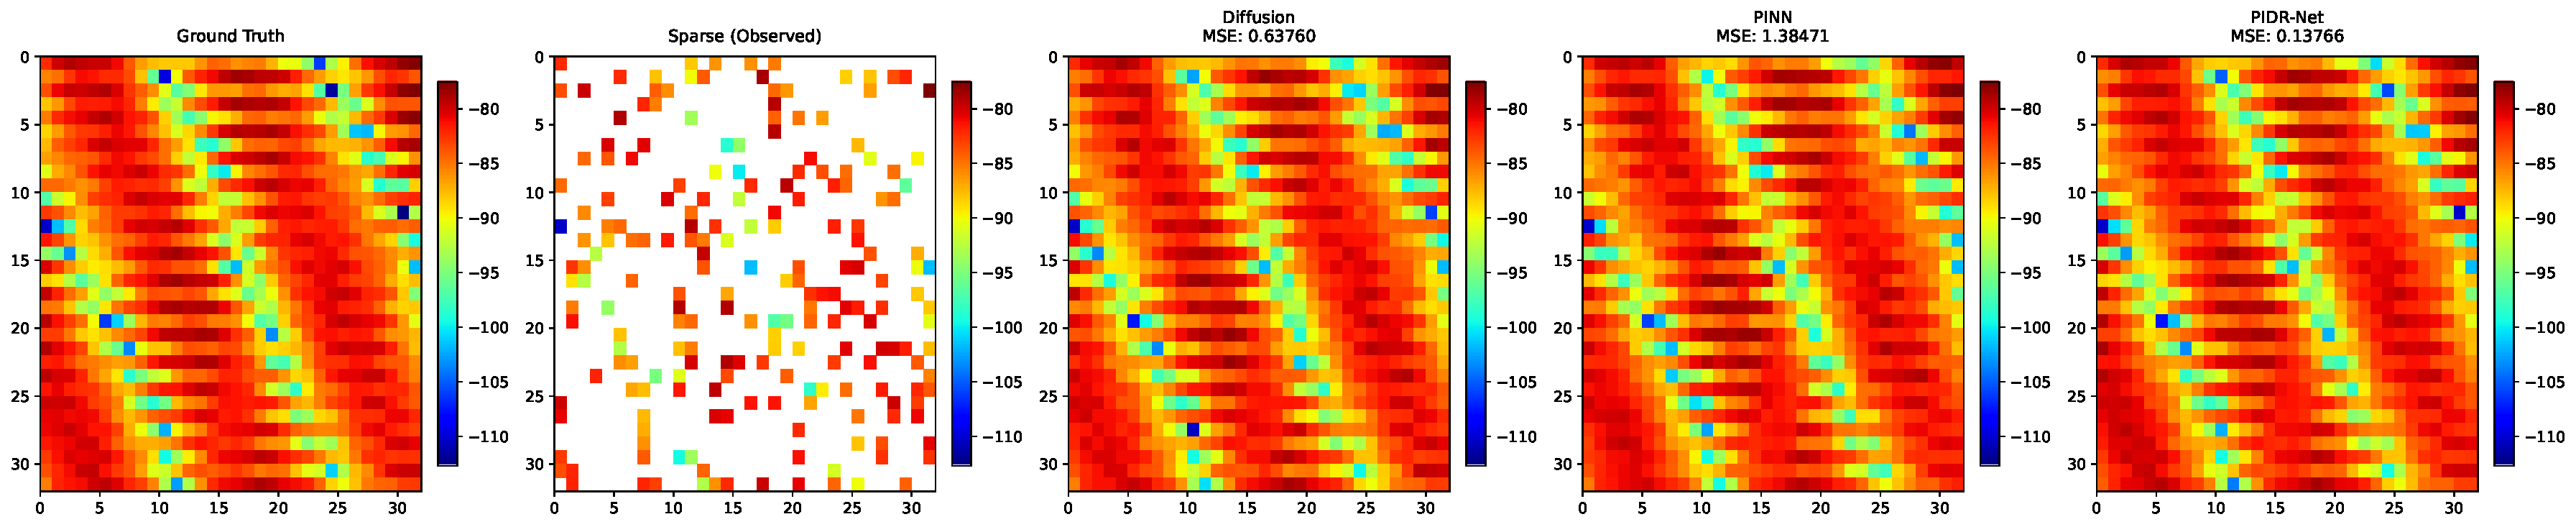
\includegraphics[width=\textwidth]{figures/recon_sample_sr.pdf}
	\caption{\protect\centering Representative qualitative comparison on the Sionna RT dataset.}
	\label{fig:rt_heatmap}
\end{figure*}

\begin{figure*}[t]
	\centering
	\captionsetup{font=footnotesize}
	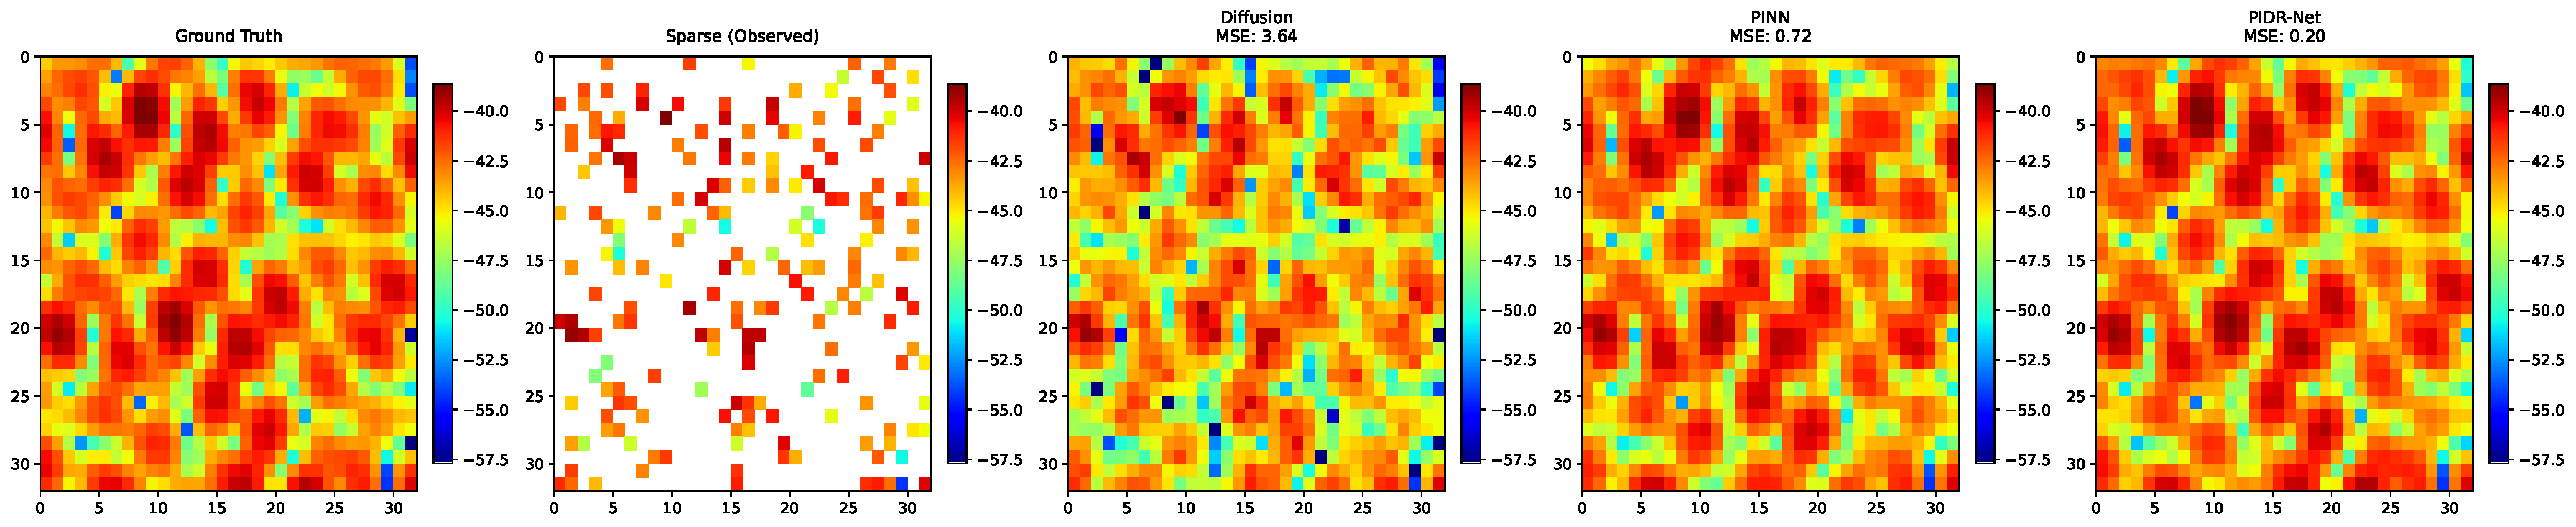
\includegraphics[width=\textwidth]{figures/recon_sample_fd.pdf}
	\caption{\protect\centering Representative qualitative comparison on the field response dataset.}
	\label{fig:field_heatmap}
\end{figure*}

\begin{figure*}[t]
	\centering
	\captionsetup{font=footnotesize}
	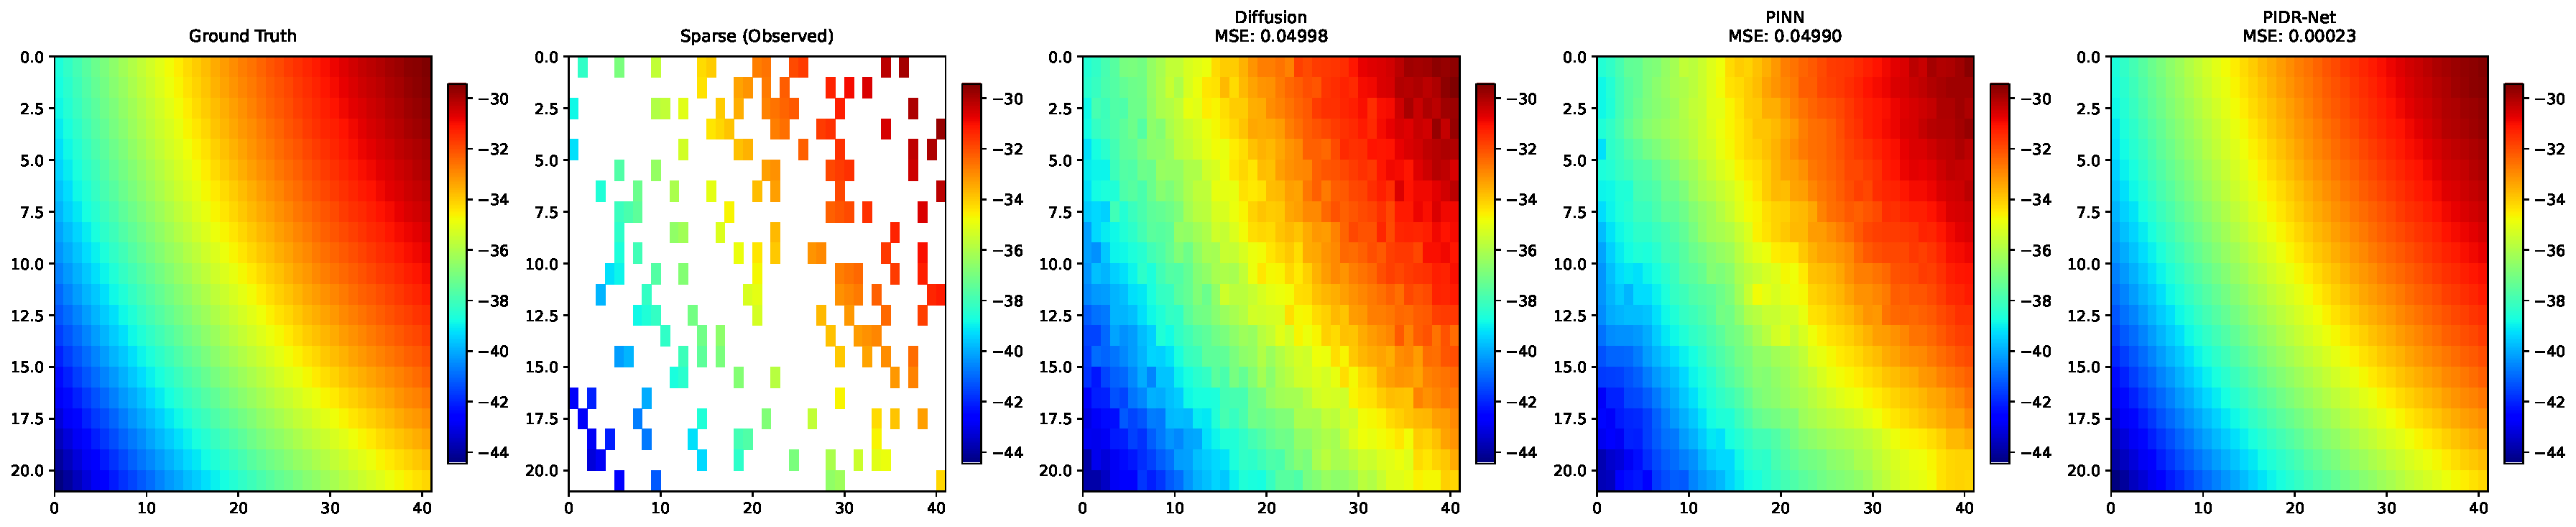
\includegraphics[width=\textwidth]{figures/recon_sample_el.pdf}
	\caption{\protect\centering Representative qualitative comparison on the EM simulation dataset.}
	\label{fig:em_heatmap}
\end{figure*}

Across the three separately trained models, the combined method ranks first on all reported reconstruction metrics. The visual examples also show that the refinement stage corrects different structures, including attenuation valleys, spurious deep fades, and grainy local errors. These results support using the same architecture with two stages for datasets with different spatial statistics.

\subsection{Impact of Different Sampling Strategies}
The preceding experiments use random sparse observations. In practical MA systems, however, sounded positions may be shaped by mechanical trajectories, blockage, access constraints, or interrupted measurements. We therefore evaluate three sampling geometries: random masking, uniform masking, and local masking. The local case is intentionally adverse, since most available pilots are concentrated in a small subregion and the unsounded area must be recovered by extrapolation rather than interpolation. Classical nearest neighbor, linear, and cubic interpolation are included in this study to benchmark the value of learned priors under nonideal sampling geometries.

For fairness, all three masking strategies are evaluated at the same observed ratio, i.e., $20\%$ of valid entries are retained and $80\%$ are missing. For each test sample, the reconstruction quality is evaluated by MSE, NMSE, PSNR, and SSIM. A representative visualization is provided in Fig.~\ref{fig:mask_strategy_heatmap}, where the ground truth, sparse observation, and reconstructed outputs are displayed side by side for all three mask patterns.

\begin{figure*}[t]
    \centering
    \captionsetup{font=footnotesize}
    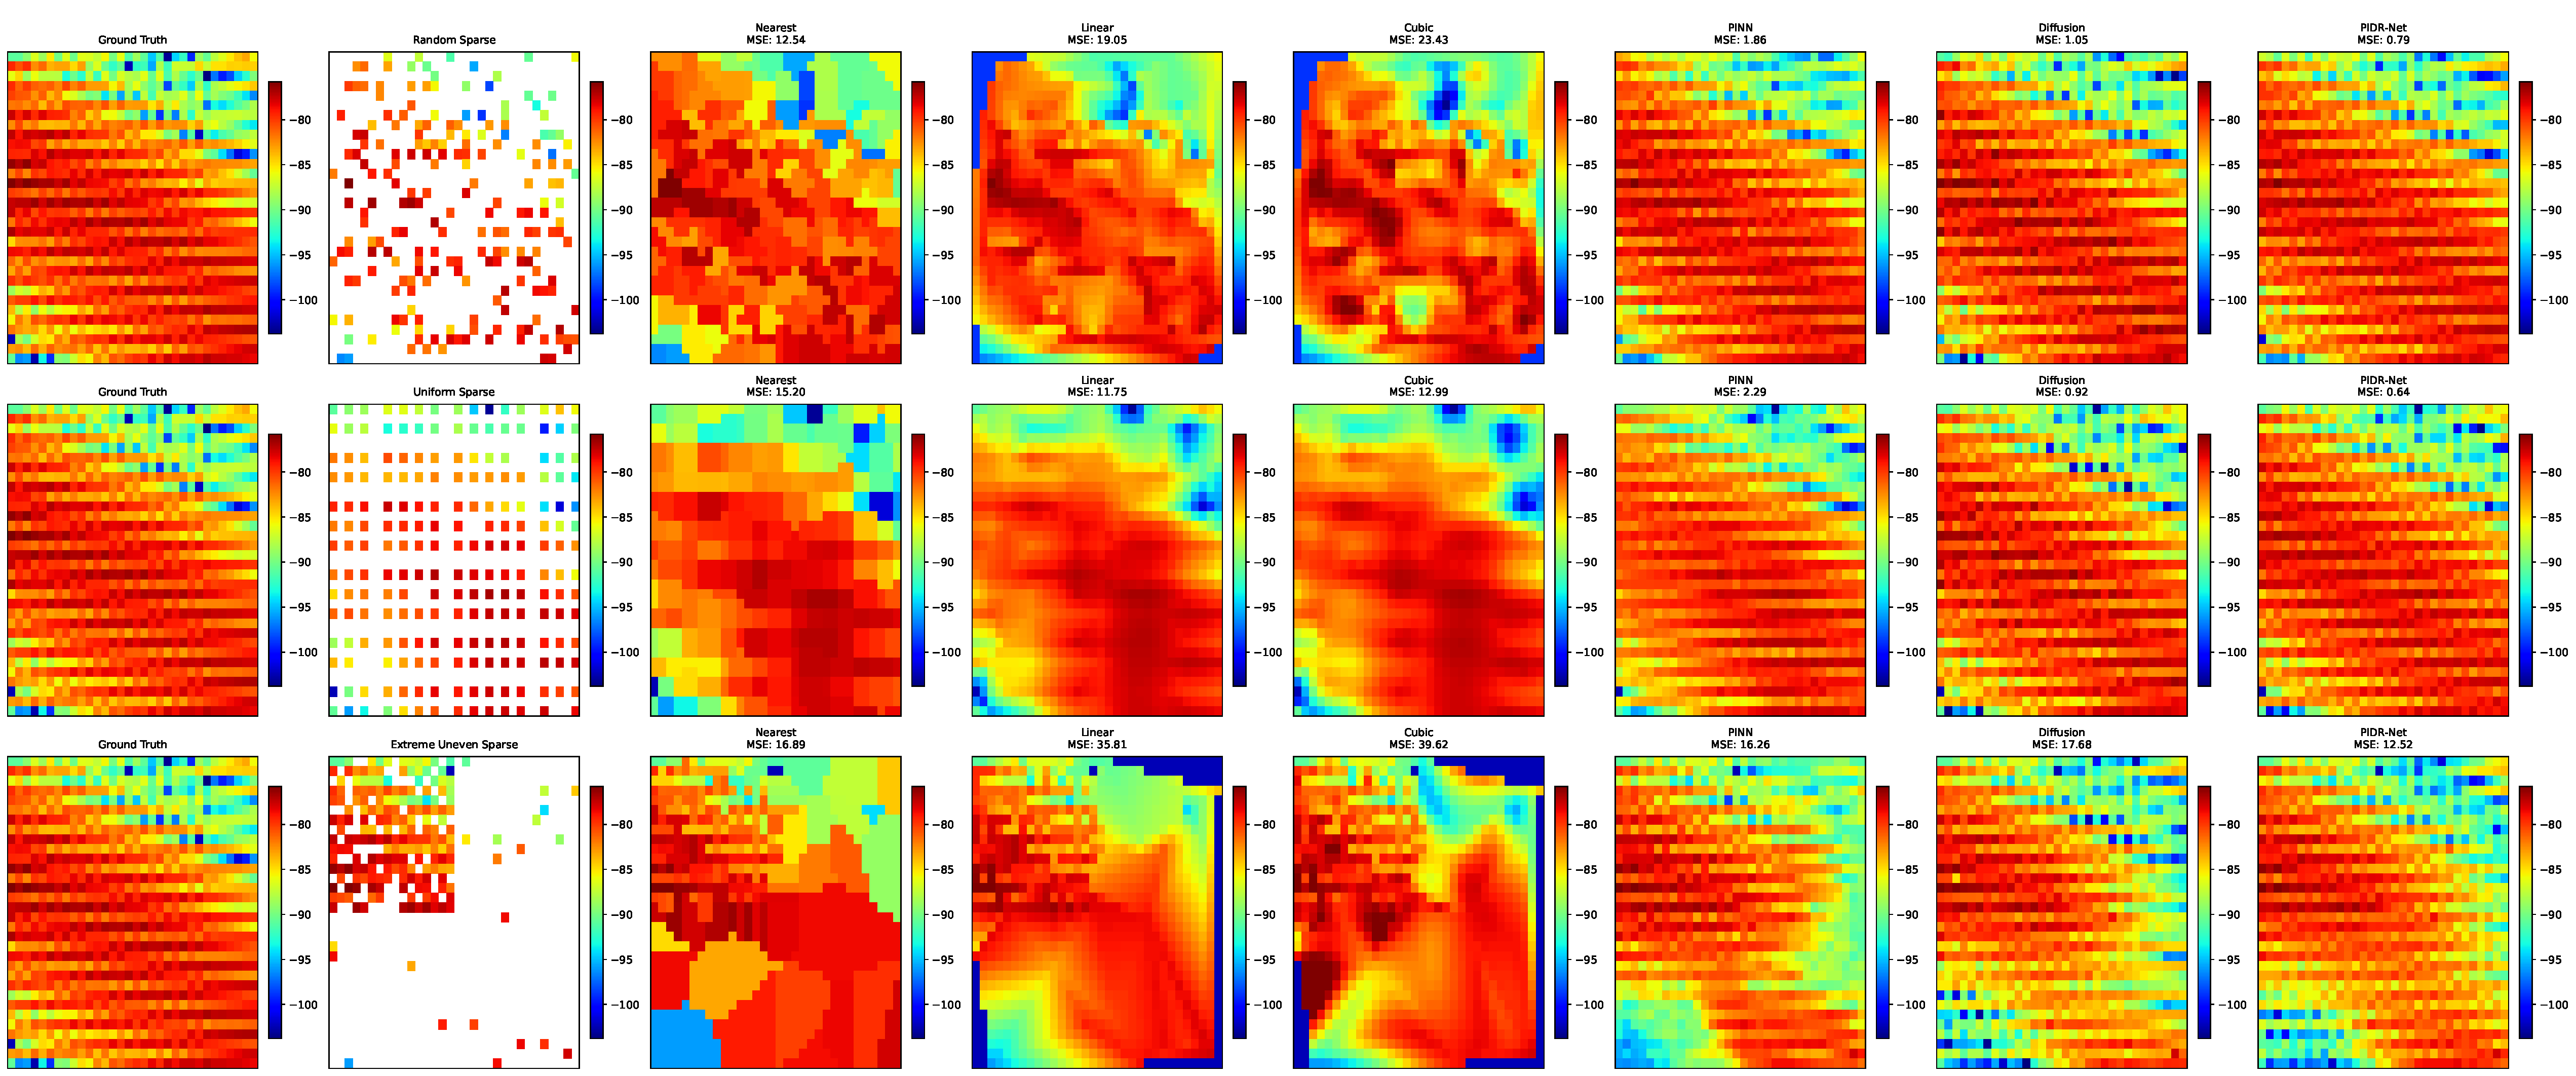
\includegraphics[width=\textwidth]{figures/mask_strategy_comparison.pdf}
    \caption{\protect\centering Representative qualitative comparison under different sampling strategies.}
    \label{fig:mask_strategy_heatmap}
\end{figure*}


The averaged quantitative results under the three masking strategies are reported in Table~\ref{tab:mask_strategy_results}, and representative visual comparisons are provided in Fig.~\ref{fig:mask_strategy_heatmap}. The average number of observed entries is kept at 205 in all cases, so that the performance difference is attributed to sampling geometry rather than measurement density.

\begin{table}[t]
	\captionsetup{font=footnotesize}
	\caption{Average quantitative results under different sampling strategies.}
	\label{tab:mask_strategy_results}
	\centering
	\scriptsize
	\setlength{\tabcolsep}{3pt}
	\resizebox{\columnwidth}{!}{%
		\begin{tabular}{llccccc}
			\toprule
			Mask strategy & Method  & MSE & NMSE (dB) & PSNR (dB) & SSIM \\
			\midrule
			\multirow{6}{*}{Random} 
			& Nearest  & 17.639 & -28.273 & 17.324 & 0.358 \\
			& Linear  & 26.056 & -26.693 & 15.744 & 0.398 \\
			& Cubic  & 31.018 & -25.891 & 14.943 & 0.359 \\
			& PINN  & 2.596 & -37.059 & 26.110 & 0.875 \\
			& Diffusion  & 1.588 & -39.821 & 28.872 & 0.929 \\
			& PIDR-Net  & $\boldsymbol{1.204}$ & $\boldsymbol{-41.643}$ & $\boldsymbol{30.694}$ & $\boldsymbol{0.954}$ \\
			\midrule
			\multirow{6}{*}{Uniform} 
			& Nearest  & 19.363 & -27.896 & 16.947 & 0.291 \\
			& Linear  & 13.797 & -29.348 & 18.399 & 0.409 \\
			& Cubic  & 15.544 & -28.862 & 17.913 & 0.373 \\
			& PINN  & 3.654 & -35.227 & 24.278 & 0.811 \\
			& Diffusion  & 1.695 & -39.404 & 28.455 & 0.919 \\
			& PIDR-Net  & $\boldsymbol{1.408}$ & $\boldsymbol{-41.066}$ & $\boldsymbol{30.117}$ & $\boldsymbol{0.943}$ \\
			
			\midrule
			\multirow{6}{*}{Local (extreme uneven)} 
			& Nearest & 22.334 & -27.119 & 16.170 & 0.339 \\
			& Linear & 91.146 & -11.269 & 11.020 & 0.340 \\
			& Cubic & 102.528 & -21.261 & 10.312 & 0.311 \\
			& PINN  & 17.948 & -27.437 & 16.489 & 0.555 \\
			& Diffusion  & $\boldsymbol{10.884}$ & $\boldsymbol{-29.913}$ & $\boldsymbol{18.965}$ & 0.784 \\
			& PIDR-Net  & 11.114 & -29.866 & 18.917 & $\boldsymbol{0.794}$ \\
			
			\bottomrule
		\end{tabular}%
	}
\end{table}

When the observations are spatially distributed, PIDR-Net gives the best results. Under random masking, it reduces the MSE from $1.588$ for diffusion and $2.596$ for PINN to $1.204$, corresponding to reductions of approximately $24.2\%$ and $53.6\%$, respectively. It also increases the SSIM from $0.929$ and $0.875$ to $0.954$. Under uniform masking, PIDR-Net again obtains the lowest MSE and NMSE and the highest PSNR and SSIM.

Local masking is more difficult because most pilots lie in one region and the rest of the map must be extrapolated. Linear and cubic interpolation give MSE values of $91.146$ and $102.528$, respectively. The learned methods produce lower errors by using patterns learned from the training maps. Diffusion has the lowest MSE in this setting, whereas PIDR-Net has the highest SSIM ($0.794$). Thus, the refiner slightly increases pointwise error relative to diffusion but preserves more of the spatial structure measured by SSIM.

Clustered measurements can arise from motion constraints, blocked sounding positions, or nonuniform probing trajectories. Under the local mask used here, PIDR-Net retains an SSIM of $0.794$, although its MSE is slightly higher than that of diffusion.

\subsection{Impact of Different Masking Ratios}
To further investigate the robustness of PIDR-Net with respect to measurement density, the missing ratio $\rho$ is varied while keeping the remaining evaluation protocol unchanged. Larger $\rho$ corresponds to fewer sounded grid positions and therefore higher online pilot saving.

The results in Table~\ref{tab:mask_ratio_results} and Fig.~\ref{fig:masking_ratio} reveal a monotonic degradation as the measurement budget decreases, which is consistent with the increasing difficulty of the inverse problem. Nevertheless, PIDR-Net maintains high structural fidelity up to $\rho=0.9$, where only $10\%$ of the grid positions are observed and the SSIM remains $0.918$. The sharper degradation at $\rho=0.95$ indicates the transition to an extremely underdetermined regime, in which the reconstruction is dominated by the learned prior and only weakly anchored by online measurements.

\begin{table}[htbp]
	\caption{PIDR-Net performance under different missing ratios.}
	\label{tab:mask_ratio_results}
	\centering
	\begin{tabular}{ccccc}
		\toprule
		Missing Ratio $\rho$ & MSE & NMSE (dB) & PSNR (dB) & SSIM \\
		\midrule
		0.7 & 0.868 & -43.536 & 32.587 & 0.966 \\
		0.8 & 1.231 & -41.638 & 30.689 & 0.954 \\
		0.9 & 2.117 & -38.620 & 27.671 & 0.918 \\
		0.95 & 9.076 & -30.827 & 19.879 & 0.605 \\
		\bottomrule
	\end{tabular}
\end{table}

\begin{figure}[htbp]
	\centering
	\captionsetup{font=footnotesize}
	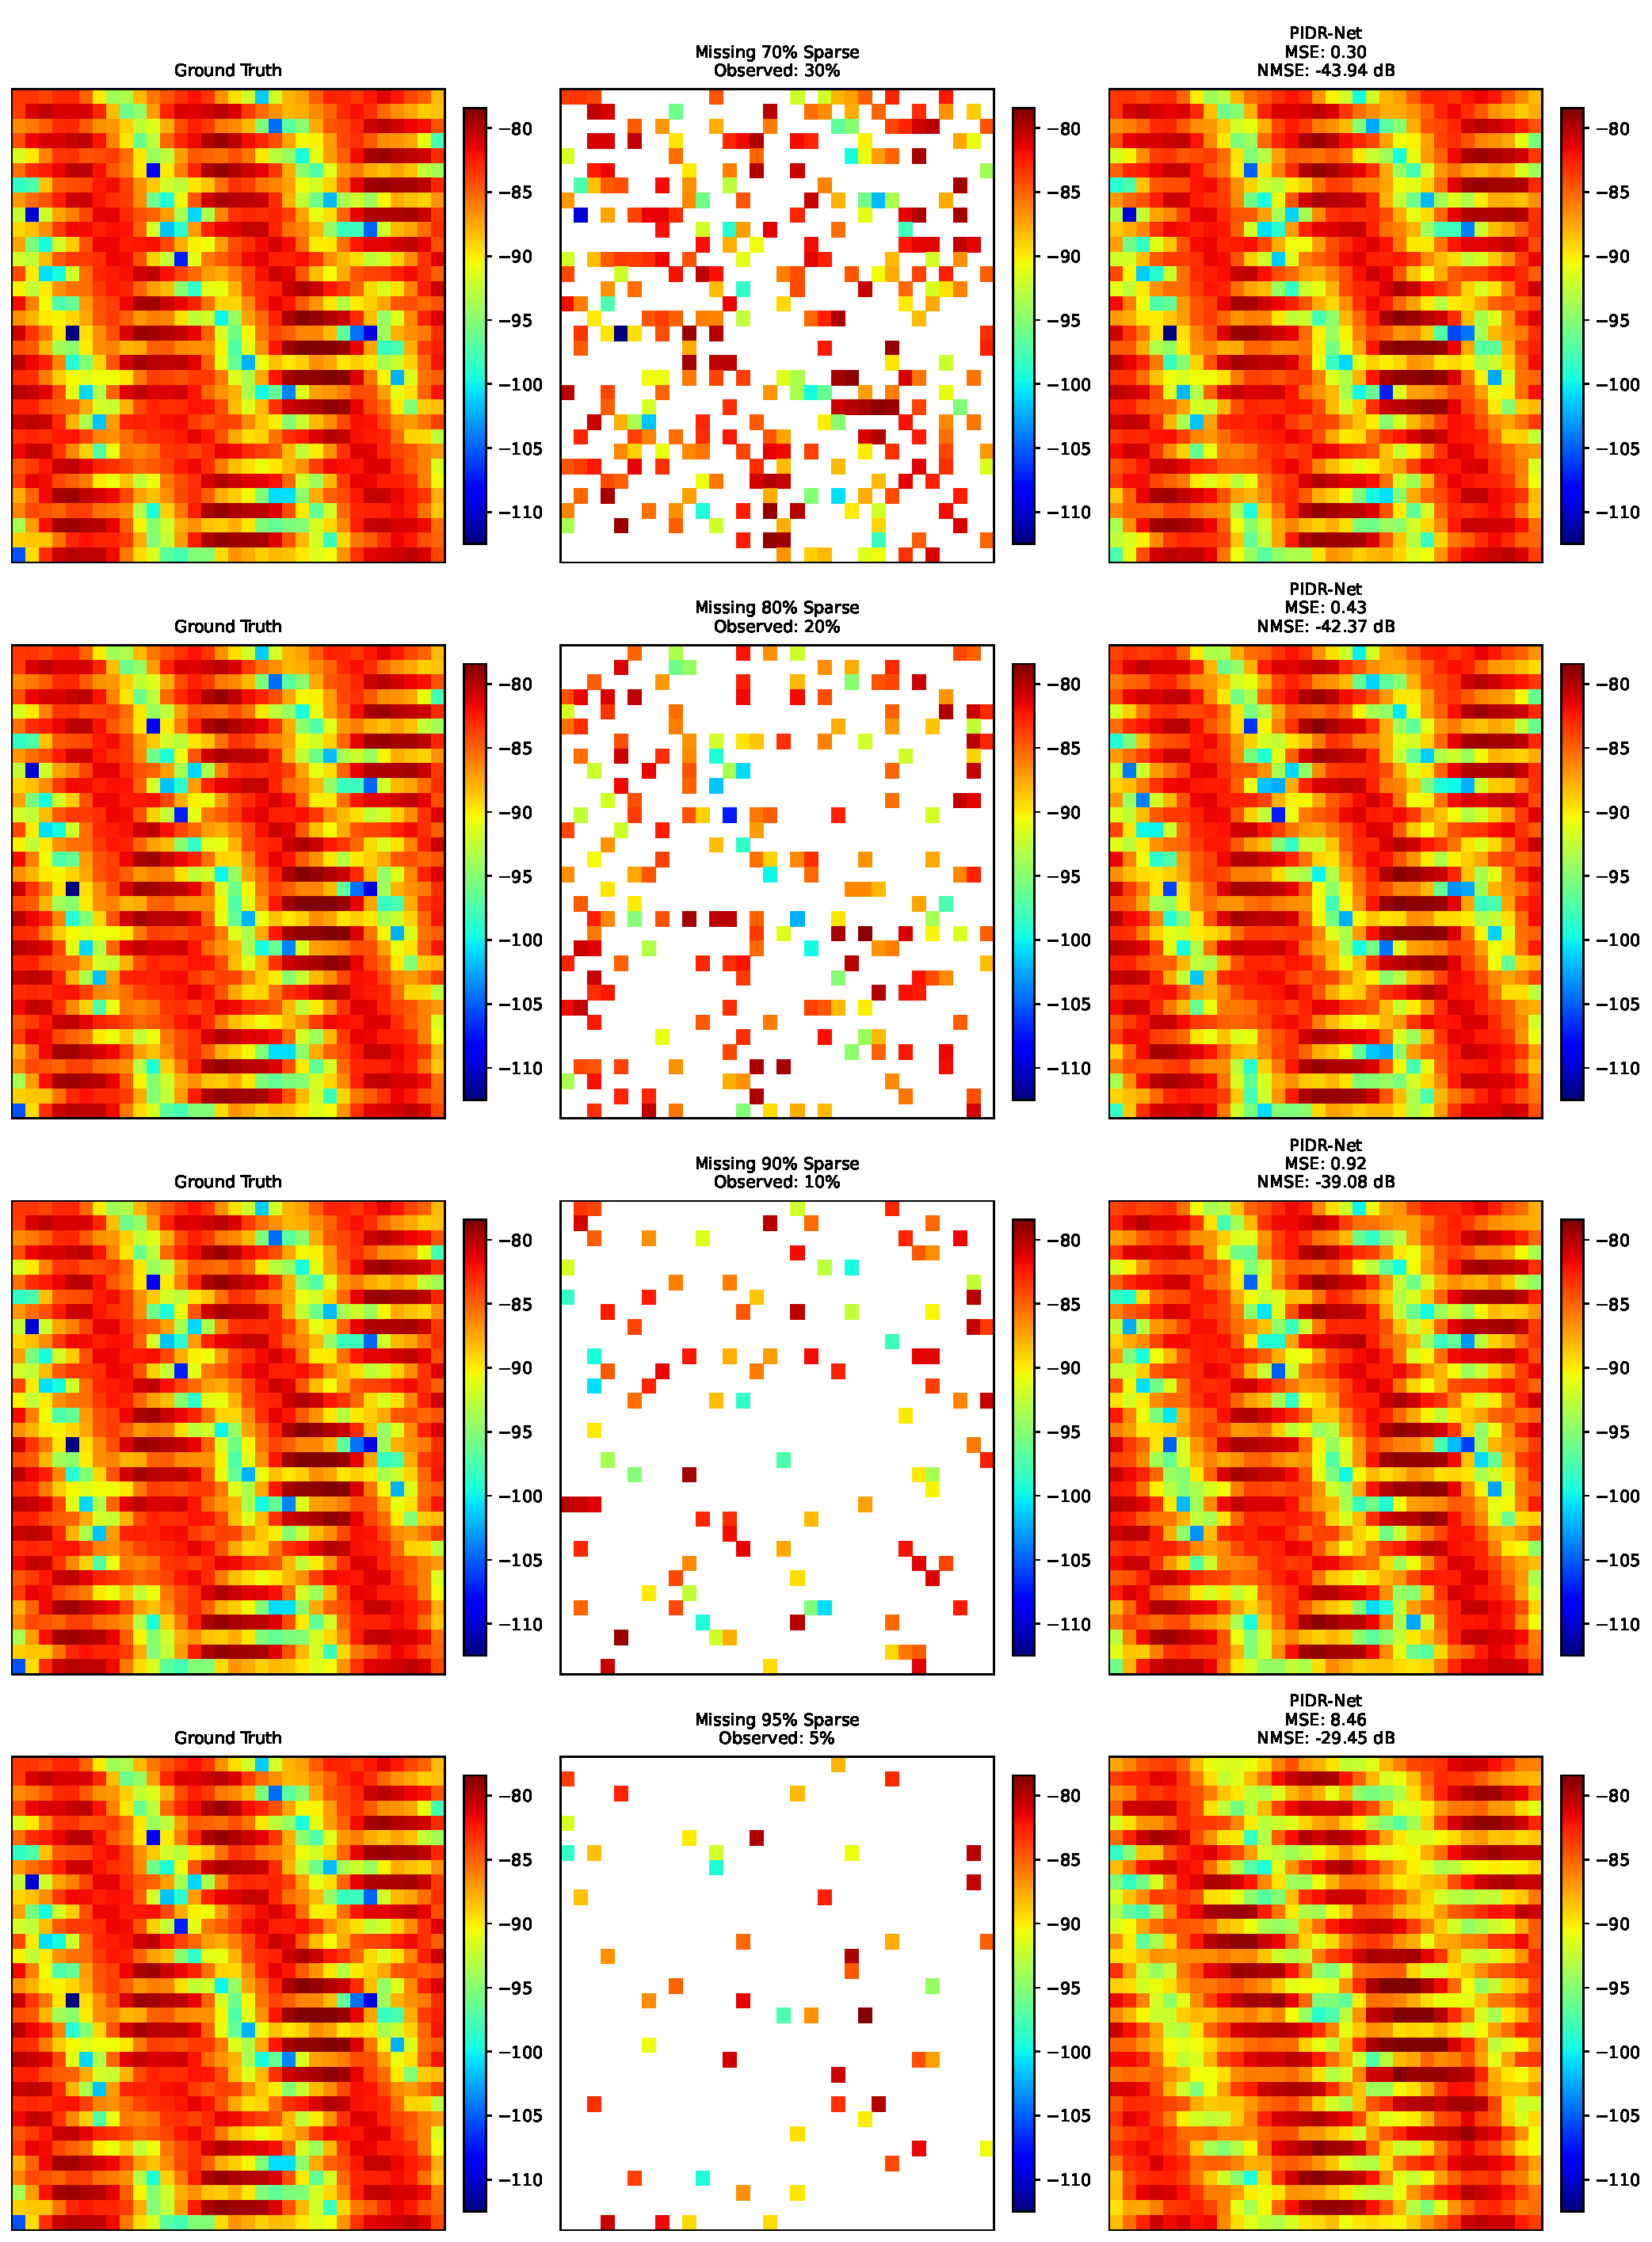
\includegraphics[width=0.48\textwidth]{figures/mask_ratio_comparison.pdf}
	\caption{\protect\centering Representative channel map recovery under different missing ratios.}
	\label{fig:masking_ratio}
\end{figure}

\subsection{Impact of Training Measurement Budget}
\label{subsec:training_budget}

The preceding missing ratio experiment varies the online measurement budget at test time while assuming fully measured offline training maps. We now evaluate the semi-supervised protocol in Section~\ref{sec:method}, which instead reduces the amount of CSI available during offline data collection. This experiment is not intended to introduce a separate model; rather, it examines how PIDR-Net behaves when the same architecture is trained with incomplete supervision.

We evaluate PIDR-Net on the Sionna RT dataset under six available ratios, $\alpha \in \{0.1, 0.2, 0.3, 0.4, 0.5, 0.6\}$. For each $\alpha$, a separate model is trained from scratch using the same training split but with only the corresponding fraction of grid points exposed. The input fraction is fixed to $\eta=0.5$, so half of the available points are used as conditioning inputs and the remaining half are used as sparse supervision labels. At test time, the input positions are drawn at random with the same density as during training, so a fraction $\alpha\eta$ of the grid is observed, from $5\%$ at $\alpha=0.1$ to $30\%$ at $\alpha=0.6$, with a fixed evaluation seed. The case $\alpha=0.4$ therefore has the same $20\%$ observation density as the fully supervised benchmark.

\begin{table}[t]
	\caption{PIDR-Net performance under different offline available ratios.}
	\label{tab:semisup_rho}
	\centering
	\small
	\setlength{\tabcolsep}{0pt}
	\begin{tabular*}{\columnwidth}{@{\extracolsep{\fill}}cccc@{}}
		\toprule
		$\alpha$ & MSE & NMSE (dB) & SSIM \\
		\midrule
		0.1 & 7.523 & $-32.124$ & 0.710 \\
		0.2 & 4.059 & -35.153 & 0.828 \\
		0.3 & 2.364 & $-37.959$ & 0.906 \\
		0.4 & 1.530 & $-40.079$ & 0.939 \\
		0.5 & 1.269 & $-41.205$ & 0.953 \\
		0.6 & 0.988 & $-42.308$ & 0.961 \\
		\bottomrule
	\end{tabular*}
\end{table}

Table~\ref{tab:semisup_rho} shows that reconstruction improves as the offline available ratio increases. At $\alpha=0.1$, the MSE is $7.523$ and the SSIM is $0.710$. At $\alpha=0.6$, the MSE decreases to $0.988$ and the SSIM increases to $0.961$. Because the test input density also grows with $\alpha$, the most direct comparison with complete training maps is $\alpha=0.4$, whose test inputs cover $20\%$ of the grid as in Table~\ref{tab:rt_main_results}. It reaches an MSE of $1.530$ and an SSIM of $0.939$, compared with $1.204$ and $0.955$ for full supervision, so sounding $40\%$ of the grid offline retains most of the accuracy obtained with complete training maps.

Fig.~\ref{fig:semisup_heatmap} compares the reconstructed gain maps at different offline available ratios. Larger values of $\alpha$ produce sharper attenuation edges and more accurate deep fading valleys, while the model trained with $\alpha=0.1$ mainly recovers the broad spatial trend. The available ratio therefore controls the measured tradeoff between offline sounding cost and reconstruction error.

\begin{figure*}[!t]
	\centering
	\captionsetup{font=footnotesize}
	\subfloat[$\alpha=0.1$]{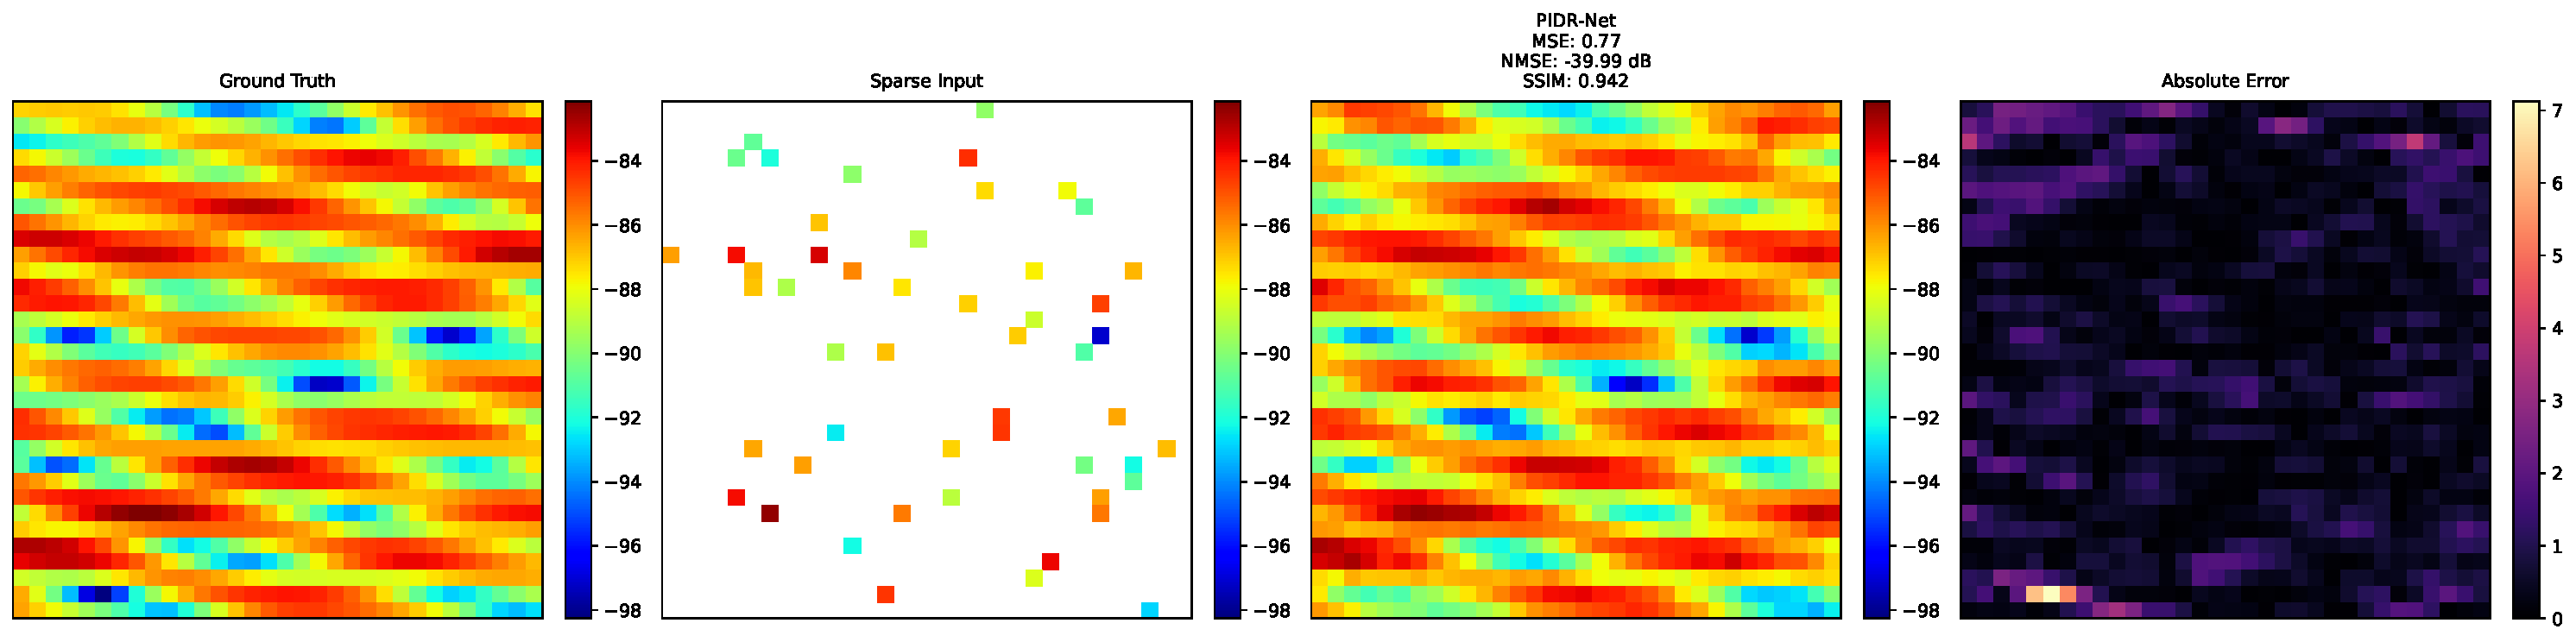
\includegraphics[width=0.32\textwidth]{figures/semisup_alpha01.pdf}}
	\hfill
	\subfloat[$\alpha=0.2$]{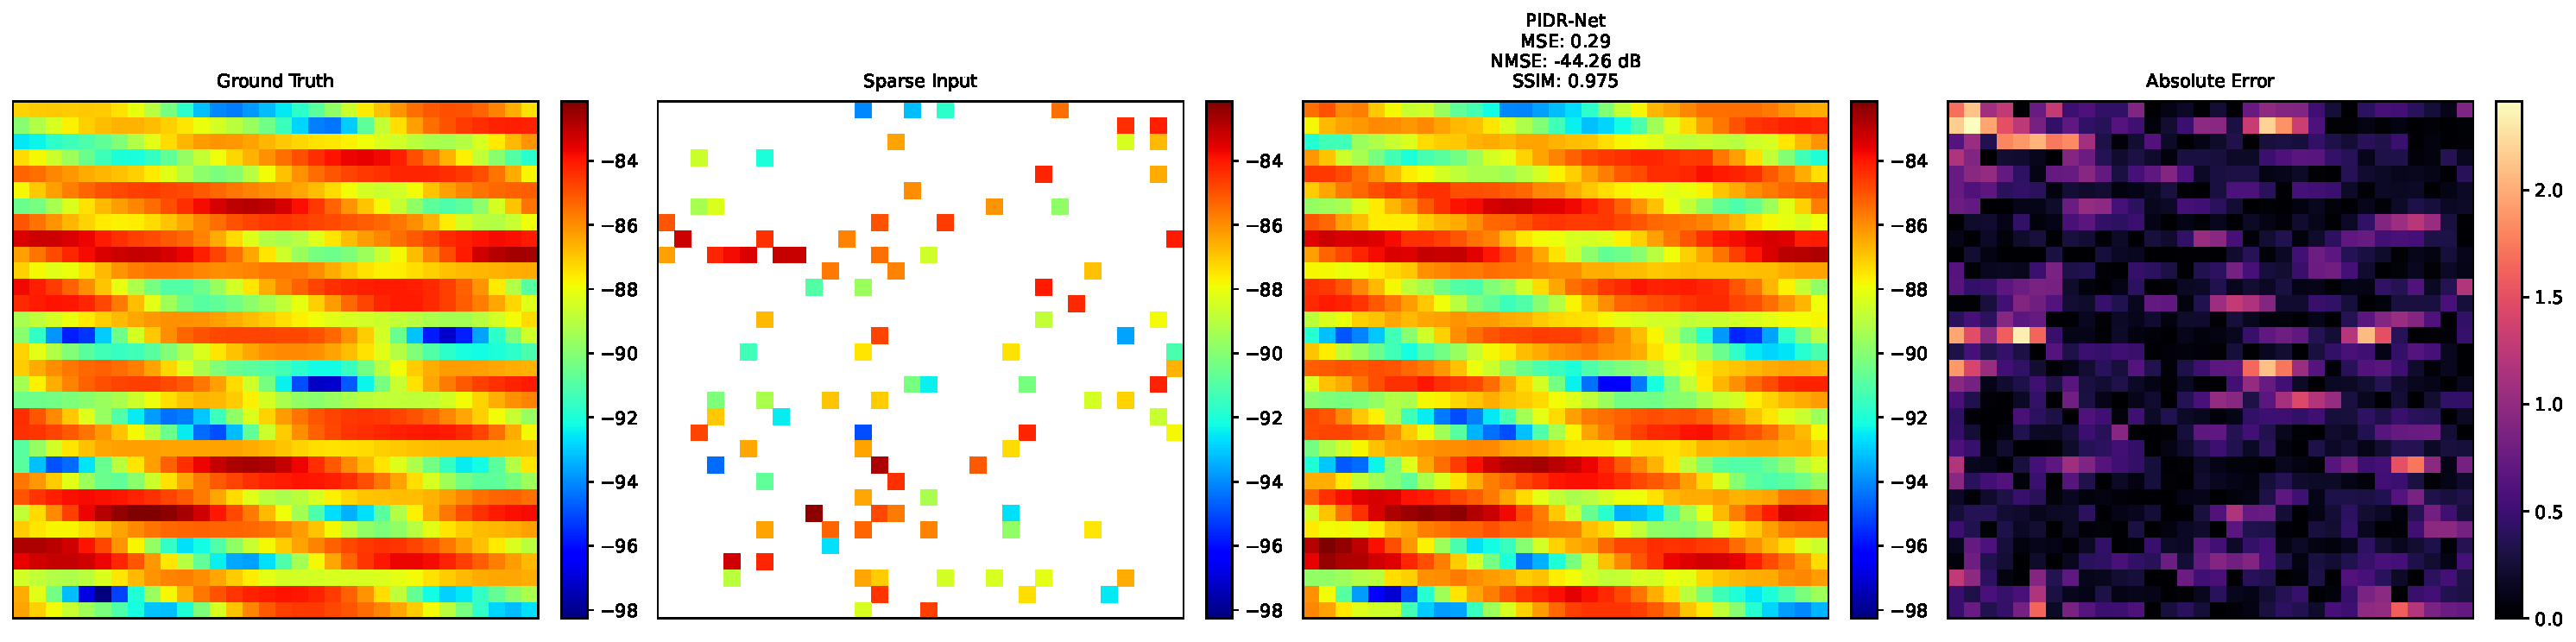
\includegraphics[width=0.32\textwidth]{figures/semisup_alpha02.pdf}}
	\hfill
	\subfloat[$\alpha=0.3$]{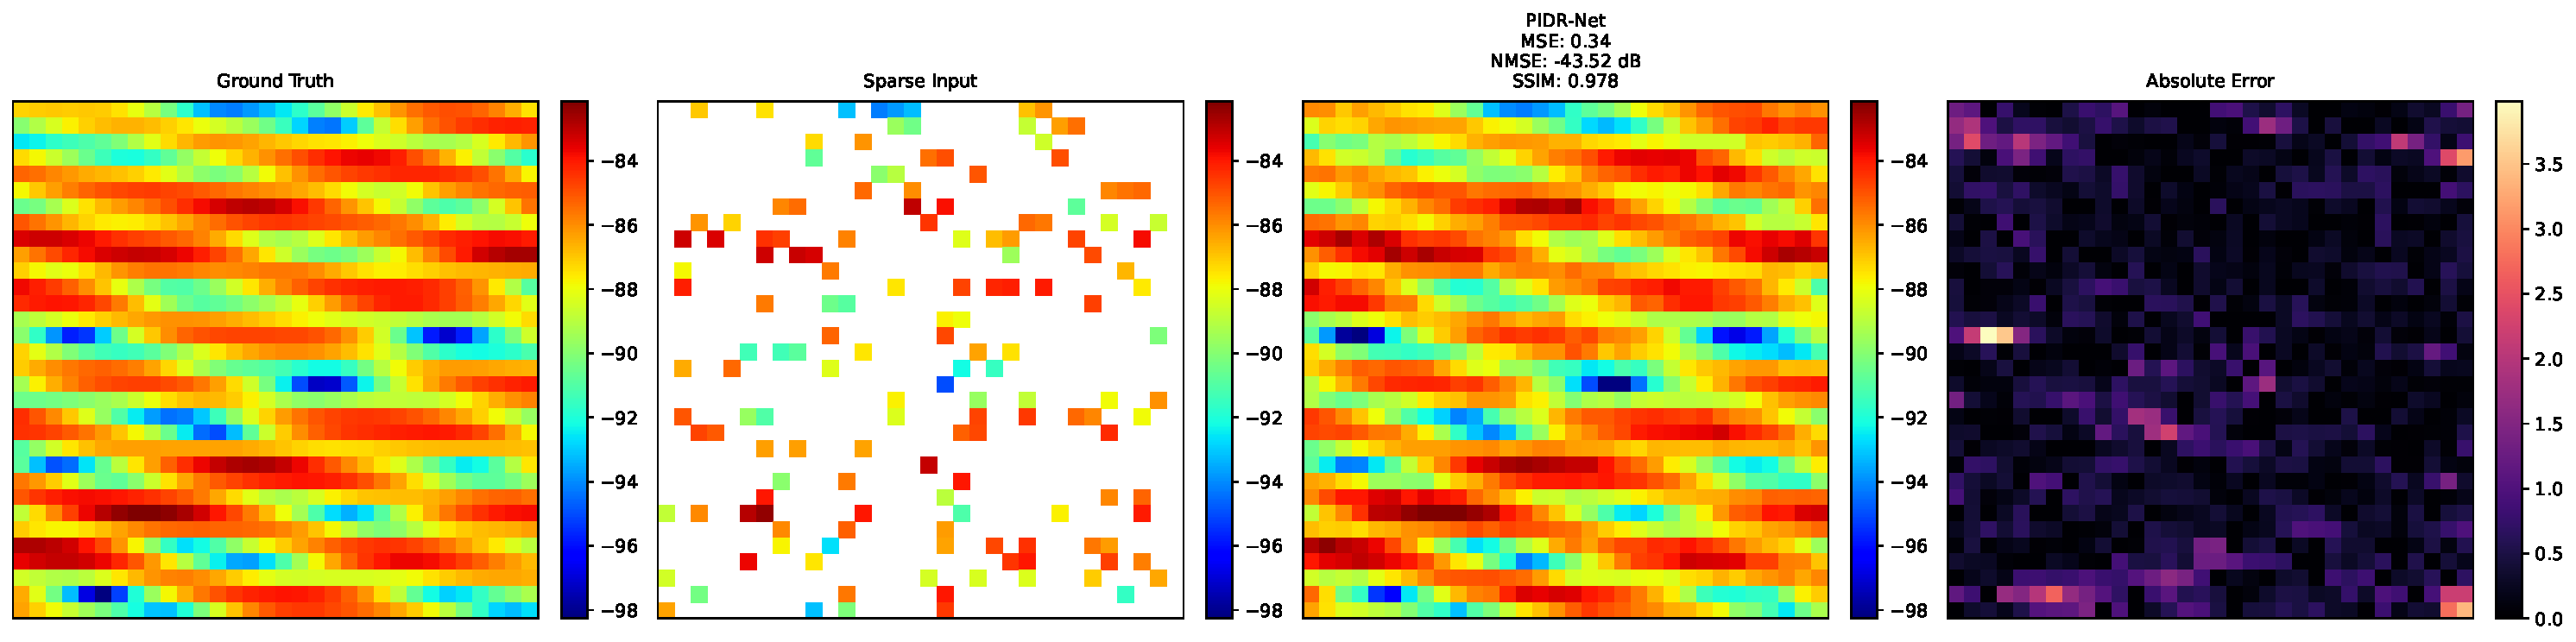
\includegraphics[width=0.32\textwidth]{figures/semisup_alpha03.pdf}}
	\par\vspace{2pt}
	\subfloat[$\alpha=0.4$]{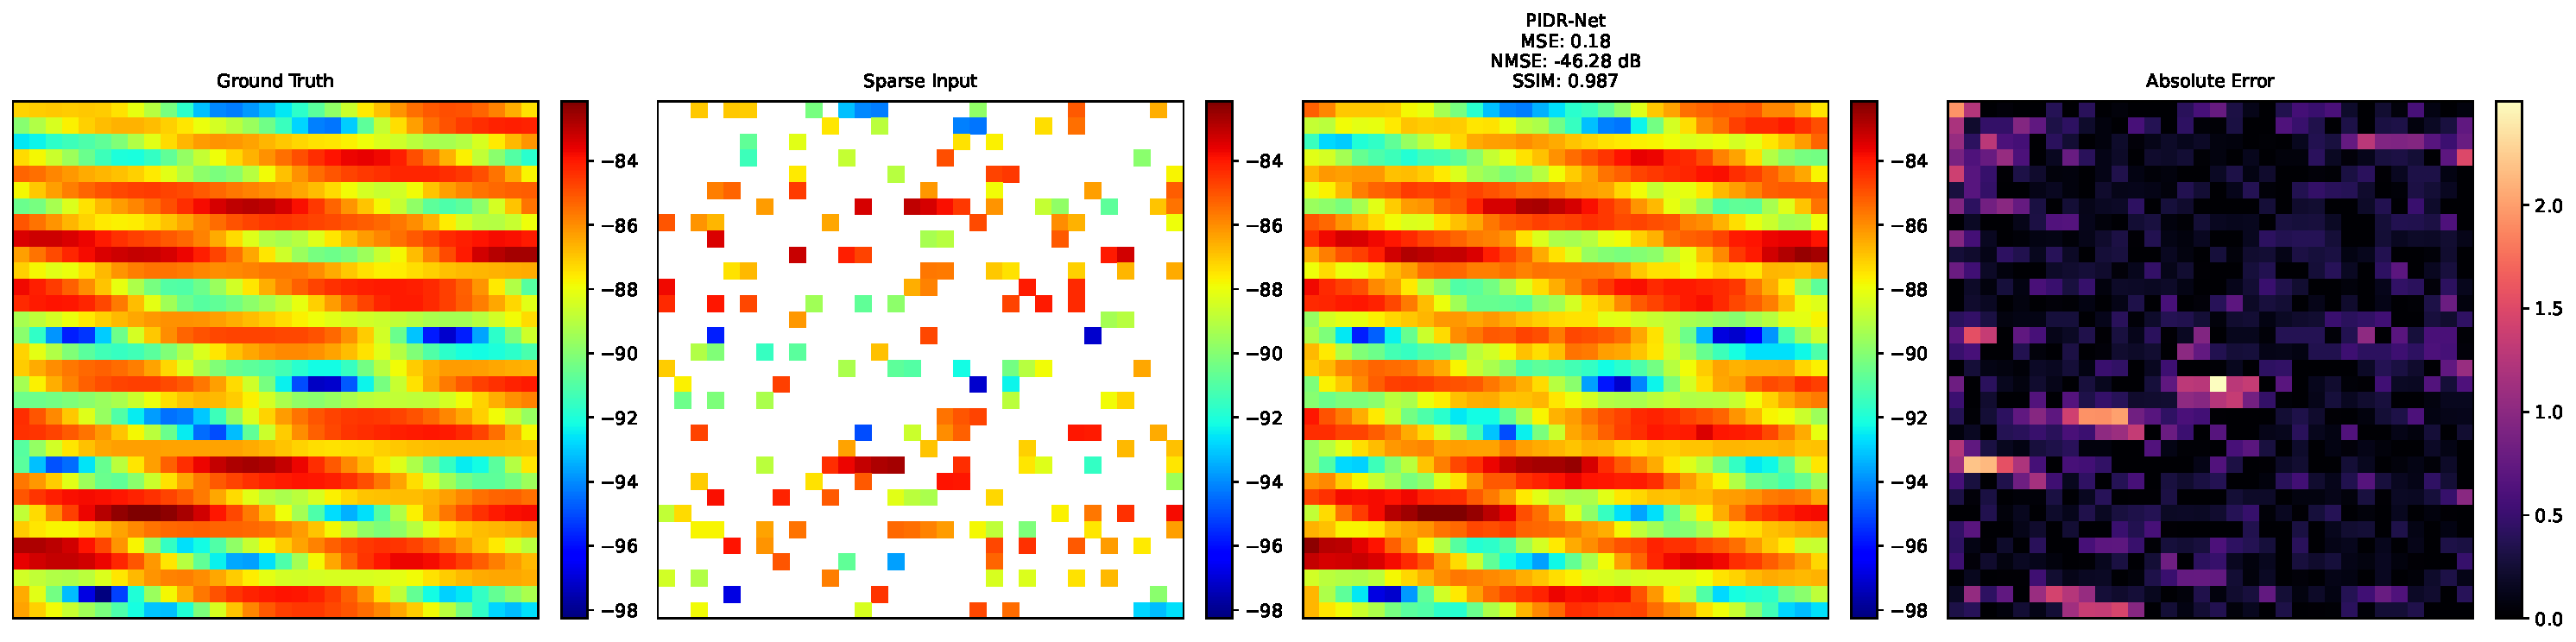
\includegraphics[width=0.32\textwidth]{figures/semisup_alpha04.pdf}}
	\hfill
	\subfloat[$\alpha=0.5$]{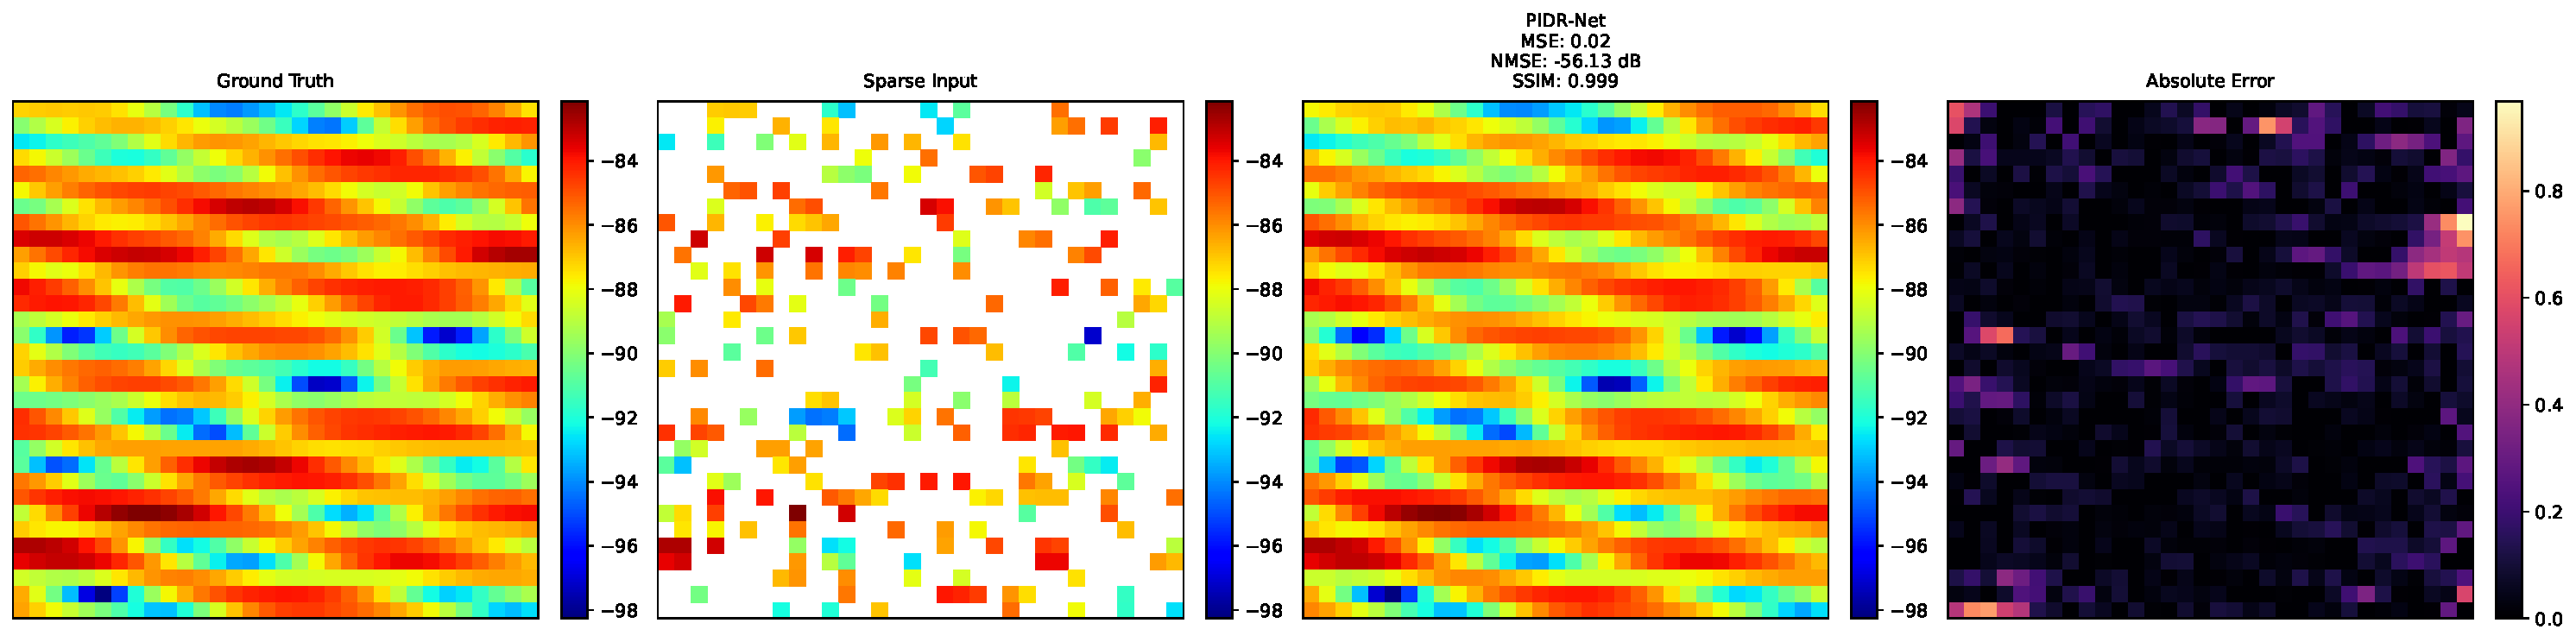
\includegraphics[width=0.32\textwidth]{figures/semisup_alpha05.pdf}}
	\hfill
	\subfloat[$\alpha=0.6$]{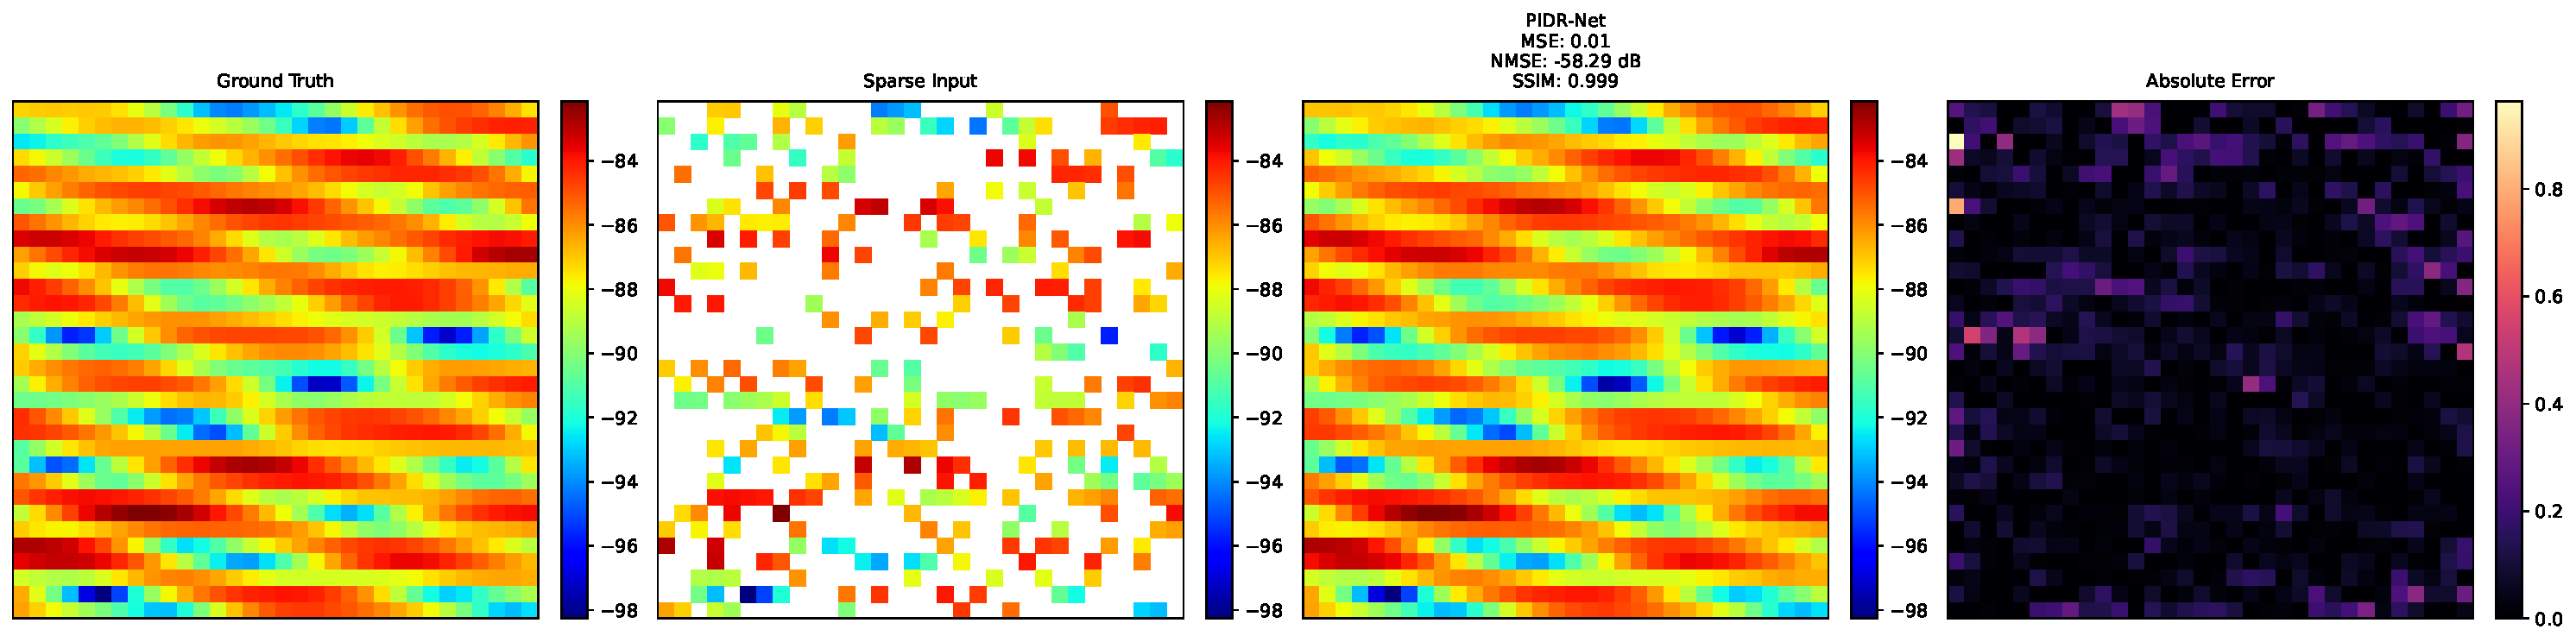
\includegraphics[width=0.32\textwidth]{figures/semisup_alpha06.pdf}}
	\caption{\protect\centering Reconstructed gain maps under different offline available ratios $\alpha$.}
	\label{fig:semisup_heatmap}
\end{figure*}

\subsection{Movable Antenna Position Optimization Based on Reconstructed CSI Maps}
\label{subsec:ma_optimization}

The preceding experiments evaluate CSI map reconstruction as a signal recovery problem. In communications with MAs, however, the reconstructed map is ultimately useful only if it supports downstream transmission decisions. We therefore examine whether the CSI maps recovered by PIDR-Net can guide antenna position optimization under a fixed transmit power budget.

We consider MA downlink settings with either one user or multiple users. The $L$ MAs are placed at distinct points on the candidate grid, and their channel coefficients are read from the corresponding user maps. The goal is to select antenna positions that improve the communication rate while satisfying a minimum spacing constraint between antennas. The constraint is enforced as a Euclidean distance in grid units; a spacing of $d_{\min}$ grid intervals corresponds to the physical distance $d_{\min}\Delta_{\mathrm t}$ and can therefore be chosen to meet a desired physical separation. The reported experiments use $d_{\min}=6$ grid units. In the case with one user, the objective is the achievable spectral efficiency of the target user. In the case with multiple users, the selected antenna positions are shared by $K$ users, and the objective becomes the sum spectral efficiency under precoding for multiple users.

Three antenna selection strategies are compared:

\begin{itemize}
	\item \textbf{Ground truth optimization (GT based):} antenna positions are selected directly using the ground truth CSI map. This serves as a reference showing the performance attainable when complete CSI maps are available during position selection.
	
	\item \textbf{PIDR based optimization:} antenna positions are optimized using the CSI map reconstructed by PIDR-Net. The resulting communication performance is evaluated on the ground truth channel map.
	
	\item \textbf{Fixed random deployment:} antenna positions are randomly selected while satisfying the spacing constraint. This scheme represents conventional nonoptimized antenna deployment and serves as the baseline method.
\end{itemize}

For the setting with one user, the candidate positions are ranked by squared channel magnitude using either the ground truth or reconstructed map. The antennas are selected greedily; after each selection, grid points violating the minimum spacing constraint are removed from the remaining candidate set. For a selected set $\mathcal{S}$, let $h_i$ denote the complex channel coefficient between the transmitter and the user when the selected MA indexed by $i$ is located at its assigned grid position. Transmit power is allocated in proportion to $|h_i|^2$, and the resulting spectral efficiency is
\begin{equation}
	\eta=\log_2\!\left(1+
	\frac{\sum_{i\in\mathcal{S}}P_i|h_i|^2}{N_0}\right),
	\qquad
	P_i=P_{\mathrm{total}}
	\frac{|h_i|^2}{\sum_{j\in\mathcal{S}}|h_j|^2},
	\label{eq:ma_rate}
\end{equation}
where $N_0$ is the noise power spectral density. The experiments use $P_{\mathrm{total}}=1$~W/Hz, $N_0=-70$~dBm/Hz, and bandwidth $B=1$~MHz. The figures report $\eta$ in bps/Hz; the corresponding data rate is $B\eta$.

For the benchmark with multiple users, the same greedy principle subject to the spacing constraint is used, but the scoring criterion is changed from the squared channel magnitude used for one user to the achieved sum spectral efficiency for multiple users. To limit the search cost, the candidate set is restricted to the $256$ grid points with the highest channel power averaged across users before greedy selection. Let $\mat{H}_{\mathcal{S}}\in\mathbb{C}^{K\times |\mathcal{S}|}$ collect the channels from the selected MA positions to the $K$ users. Maximum ratio transmission (MRT) beams are formed from the CSI map used by the corresponding selection strategy. For user $k$, the SINR is evaluated on the ground truth channel as
\begin{equation}
	\mathrm{SINR}_k=
	\frac{P_k|\vect{h}_k^T\vect{w}_k|^2}
	{\sum_{\ell\ne k}P_{\ell}|\vect{h}_k^T\vect{w}_{\ell}|^2+N_0},
	\label{eq:multiuser_sinr}
\end{equation}
where $\vect{h}_k\in\mathbb{C}^{|\mathcal{S}|}$ is the ground truth channel vector from the selected MA positions to user $k$, i.e., the transpose of row $k$ of $\mat{H}_{\mathcal{S}}$. Under the adopted downlink convention, the MRT beam $\vect{w}_k\in\mathbb{C}^{|\mathcal{S}|}$ is given by $\vect{w}_k=\vect{h}_{k,\mathrm{sel}}^*/\norm{\vect{h}_{k,\mathrm{sel}}}_2$, where $\vect{h}_{k,\mathrm{sel}}\in\mathbb{C}^{|\mathcal{S}|}$ is obtained from the CSI map used by the corresponding selection strategy. Thus, the effective channel is written as $\vect{h}_k^T\vect{w}_{\ell}$. The interference index in \eqref{eq:multiuser_sinr} satisfies $\ell\in\{1,\ldots,K\}\setminus\{k\}$. Here, $P_k=P_{\mathrm{total}}/K$ is the transmit power spectral density allocated to user $k$, so equal power allocation is used across the $K$ users. The selection objective for multiple users is
\begin{equation}
	R_{\mathrm{sum}}=\sum_{k=1}^{K}\log_2(1+\mathrm{SINR}_k).
	\label{eq:multiuser_sum_rate}
\end{equation}
When PIDR based optimization is used, both the antenna positions and MRT beams are determined from the reconstructed CSI maps, while the final SINR and rate are evaluated on the ground truth channels. This evaluation protocol tests whether the reconstructed maps preserve not only pointwise CSI values but also the spatial ranking and channel structure across users needed for downstream MA deployment.

For the case with one user, two representative antenna configurations are considered, namely $L=4$ and $L=8$. The corresponding CSI map based antenna optimization results on the Sionna RT dataset are illustrated in Fig.~\ref{fig:ma_singleuser_comparison}.

\begin{figure*}[!t]
	\centering
	\captionsetup{font=footnotesize}
	\subfloat[$L=4$]{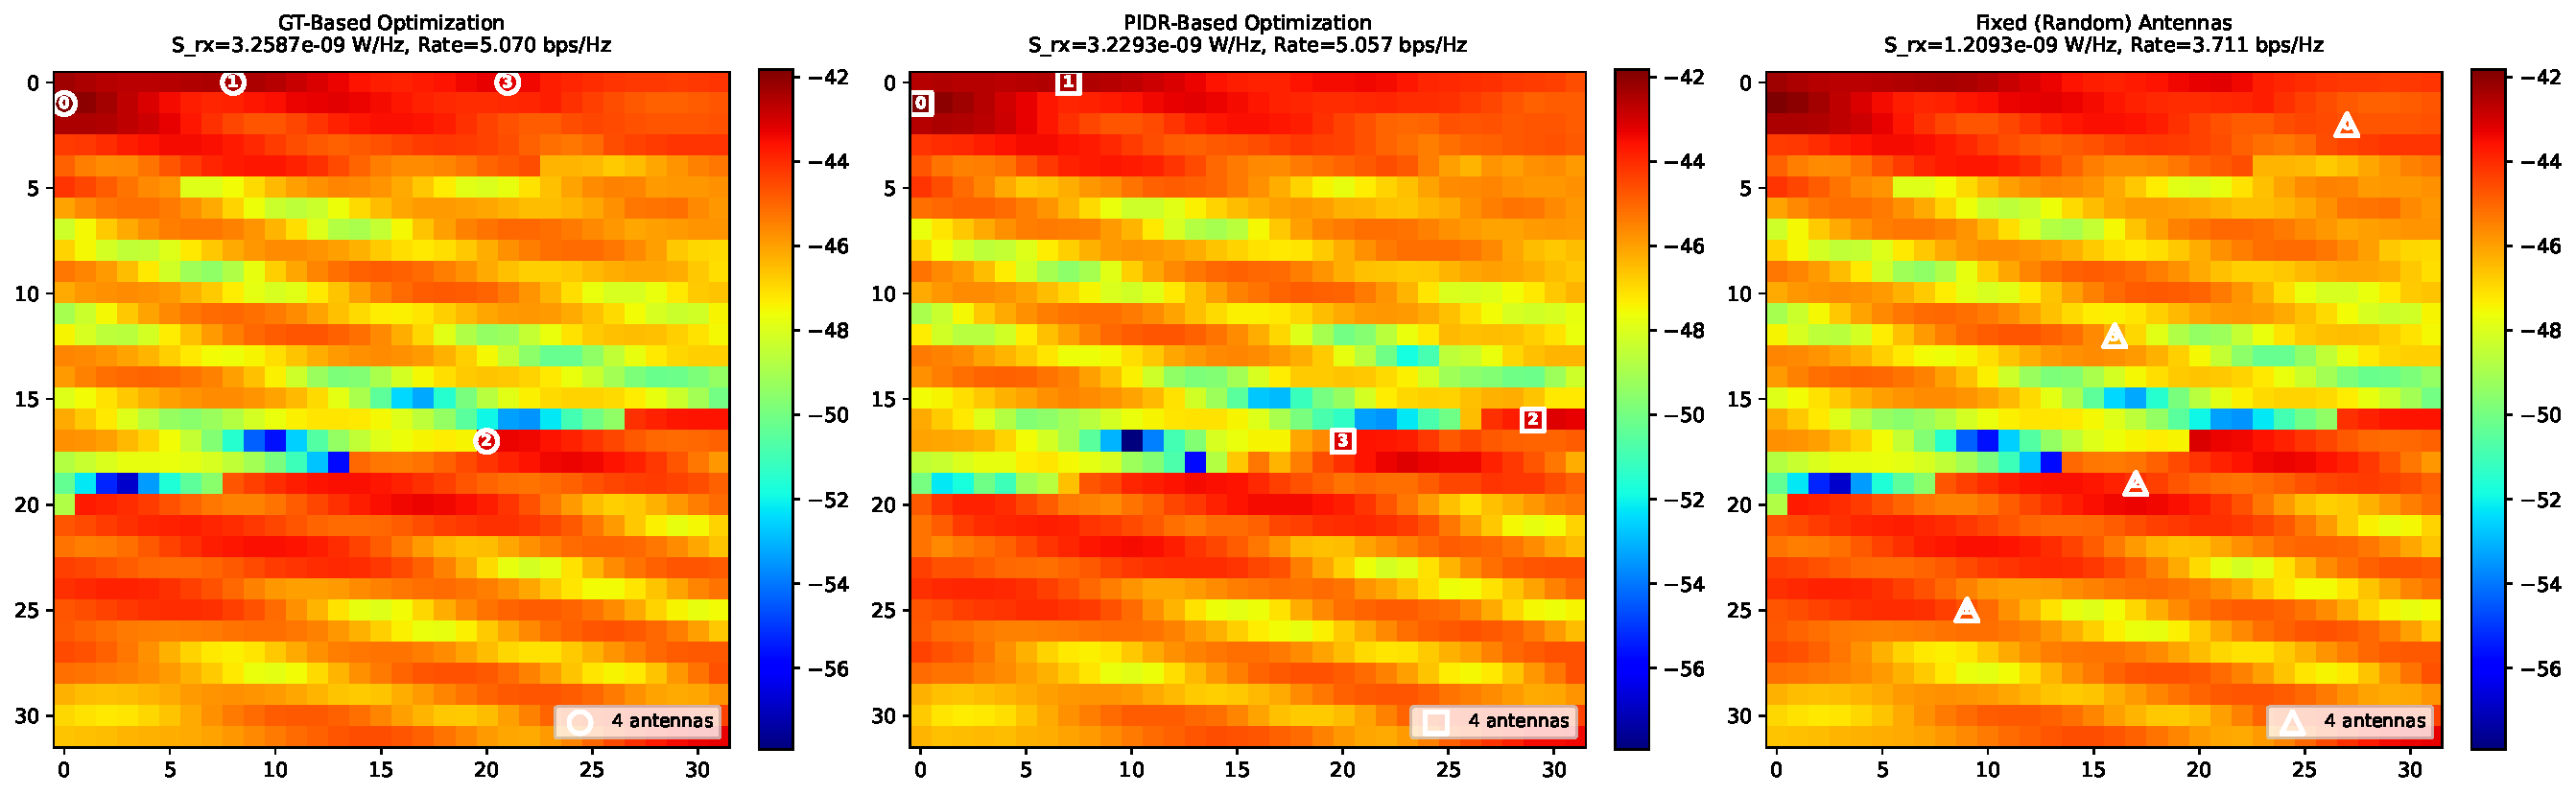
\includegraphics[width=0.48\textwidth]{figures/ma_single_user_L4.pdf}}
	\hfill
	\subfloat[$L=8$]{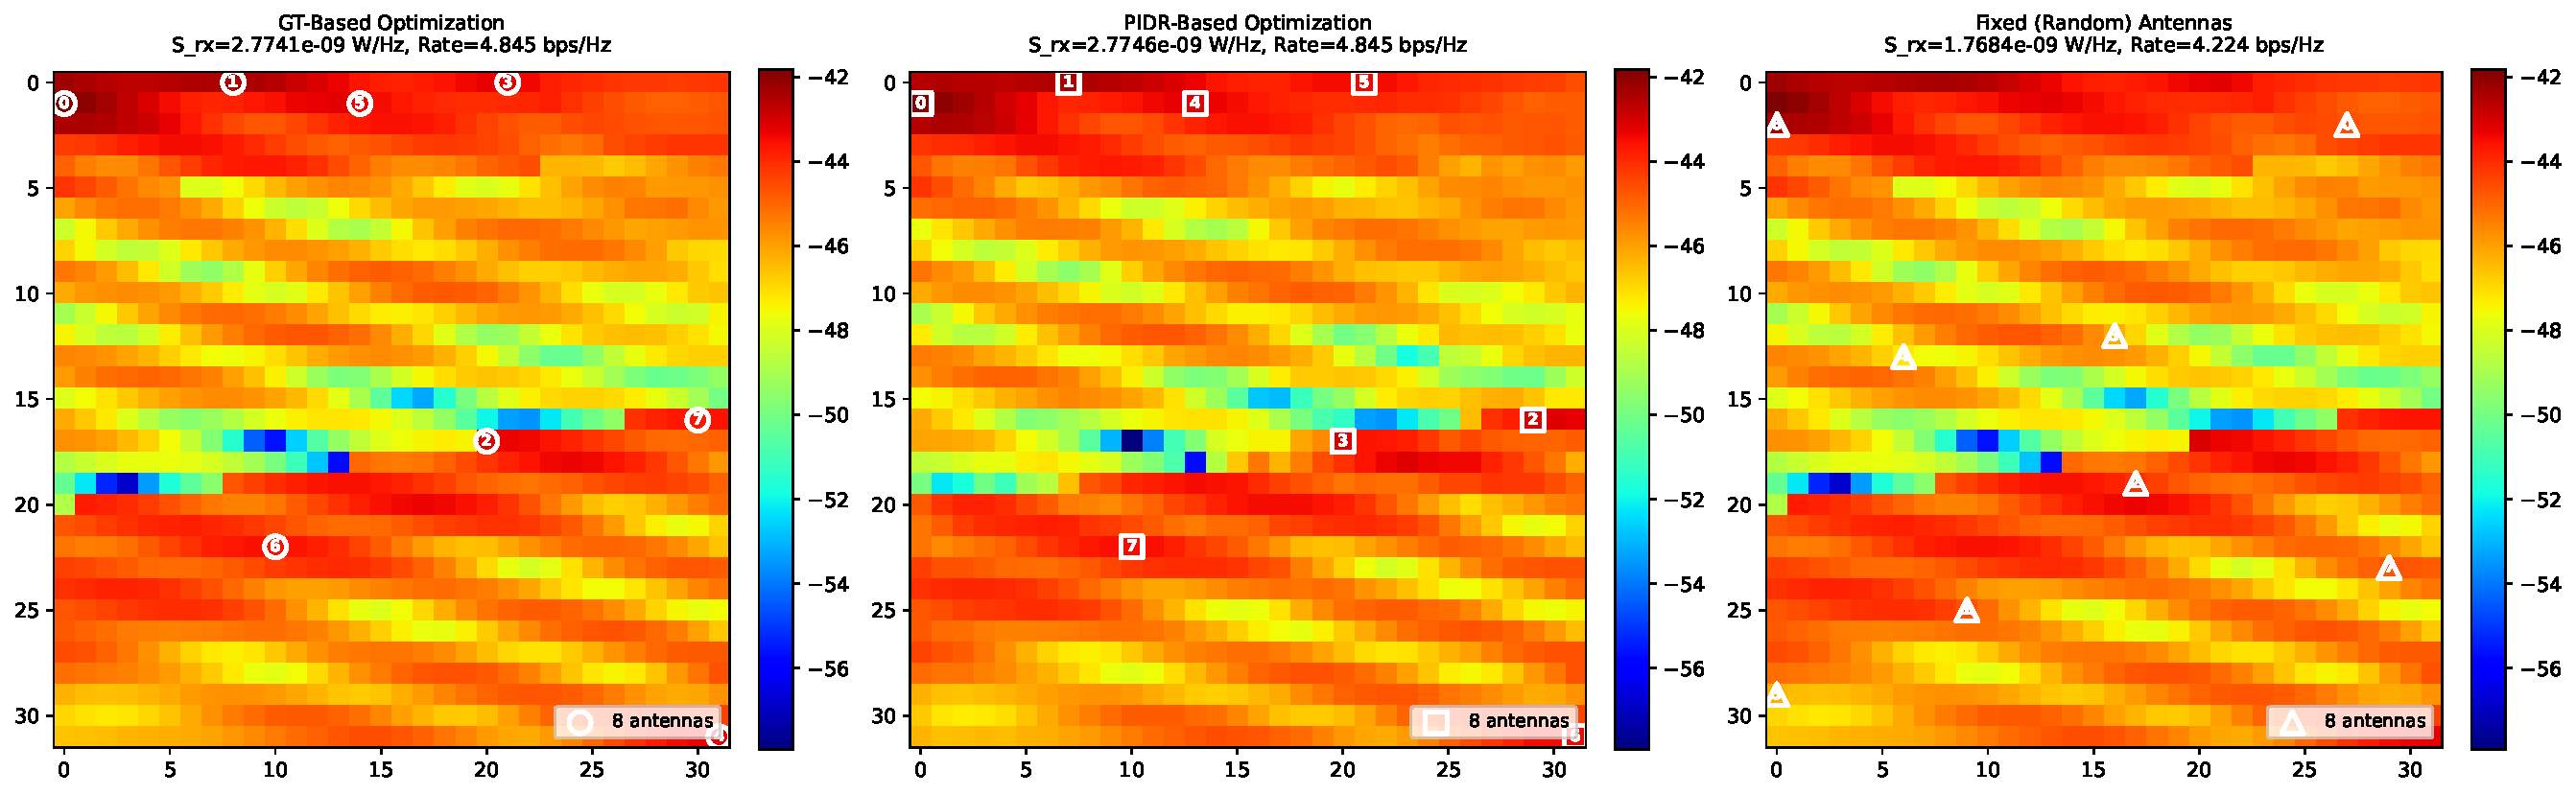
\includegraphics[width=0.48\textwidth]{figures/ma_single_user_L8.pdf}}
	\caption{\protect\centering MA position optimization for one user on the Sionna RT dataset.}
	\label{fig:ma_singleuser_comparison}
\end{figure*}

The setting with multiple users is further evaluated on the Sionna RT, field response, and EM simulation datasets with $K=3$ users and $L=4$ movable antennas. The quantitative comparison is summarized in Table~\ref{tab:ma_multiuser_results}, and the corresponding visual results are shown in Fig.~\ref{fig:ma_multiuser_comparison}. Across the three datasets, PIDR based optimization consistently outperforms fixed random deployment in terms of sum spectral efficiency. On the Sionna RT and EM simulation datasets, the PIDR based rates are close to the GT based reference, indicating that the reconstructed maps preserve the dominant spatial structure across users. On the field response dataset, the PIDR based greedy selection obtains a slightly higher evaluated sum rate than the GT based greedy reference. This does not imply that PIDR surpasses complete CSI in a global optimization sense; rather, it reflects the heuristic nature of the greedy search subject to the spacing constraint and the fact that different CSI maps can induce different locally favorable search trajectories.

\begin{table*}[t]
	\caption{MA position optimization results for multiple users on three datasets.}
	\label{tab:ma_multiuser_results}
	\centering
	\small
	\setlength{\tabcolsep}{5pt}
	\begin{tabular}{llccc}
		\toprule
		Dataset & Method & Sum spectral efficiency (bps/Hz) & Mean SINR (dB) & Minimum SINR (dB) \\
		\midrule
		\multirow{3}{*}{Sionna RT}
		& GT based & 3.361 & 0.531 & -0.868 \\
		& PIDR based & 2.956 & -0.138 & -1.274 \\
		& Fixed random & 2.348 & -1.440 & -1.805 \\
		\midrule
		\multirow{3}{*}{Field response}
		& GT based & 9.702 & 9.226 & 7.476 \\
		& PIDR based & 10.516 & 10.142 & 9.148 \\
		& Fixed random & 3.001 & -0.134 & -2.208 \\
		\midrule
		\multirow{3}{*}{EM simulation}
		& GT based & 2.884 & -0.326 & -1.498 \\
		& PIDR based & 2.765 & -0.557 & -1.611 \\
		& Fixed random & 2.255 & -1.670 & -2.211 \\
		\bottomrule
	\end{tabular}
\end{table*}

\begin{figure*}[t]
	\centering
	\captionsetup{font=footnotesize}
	\subfloat[Sionna RT]{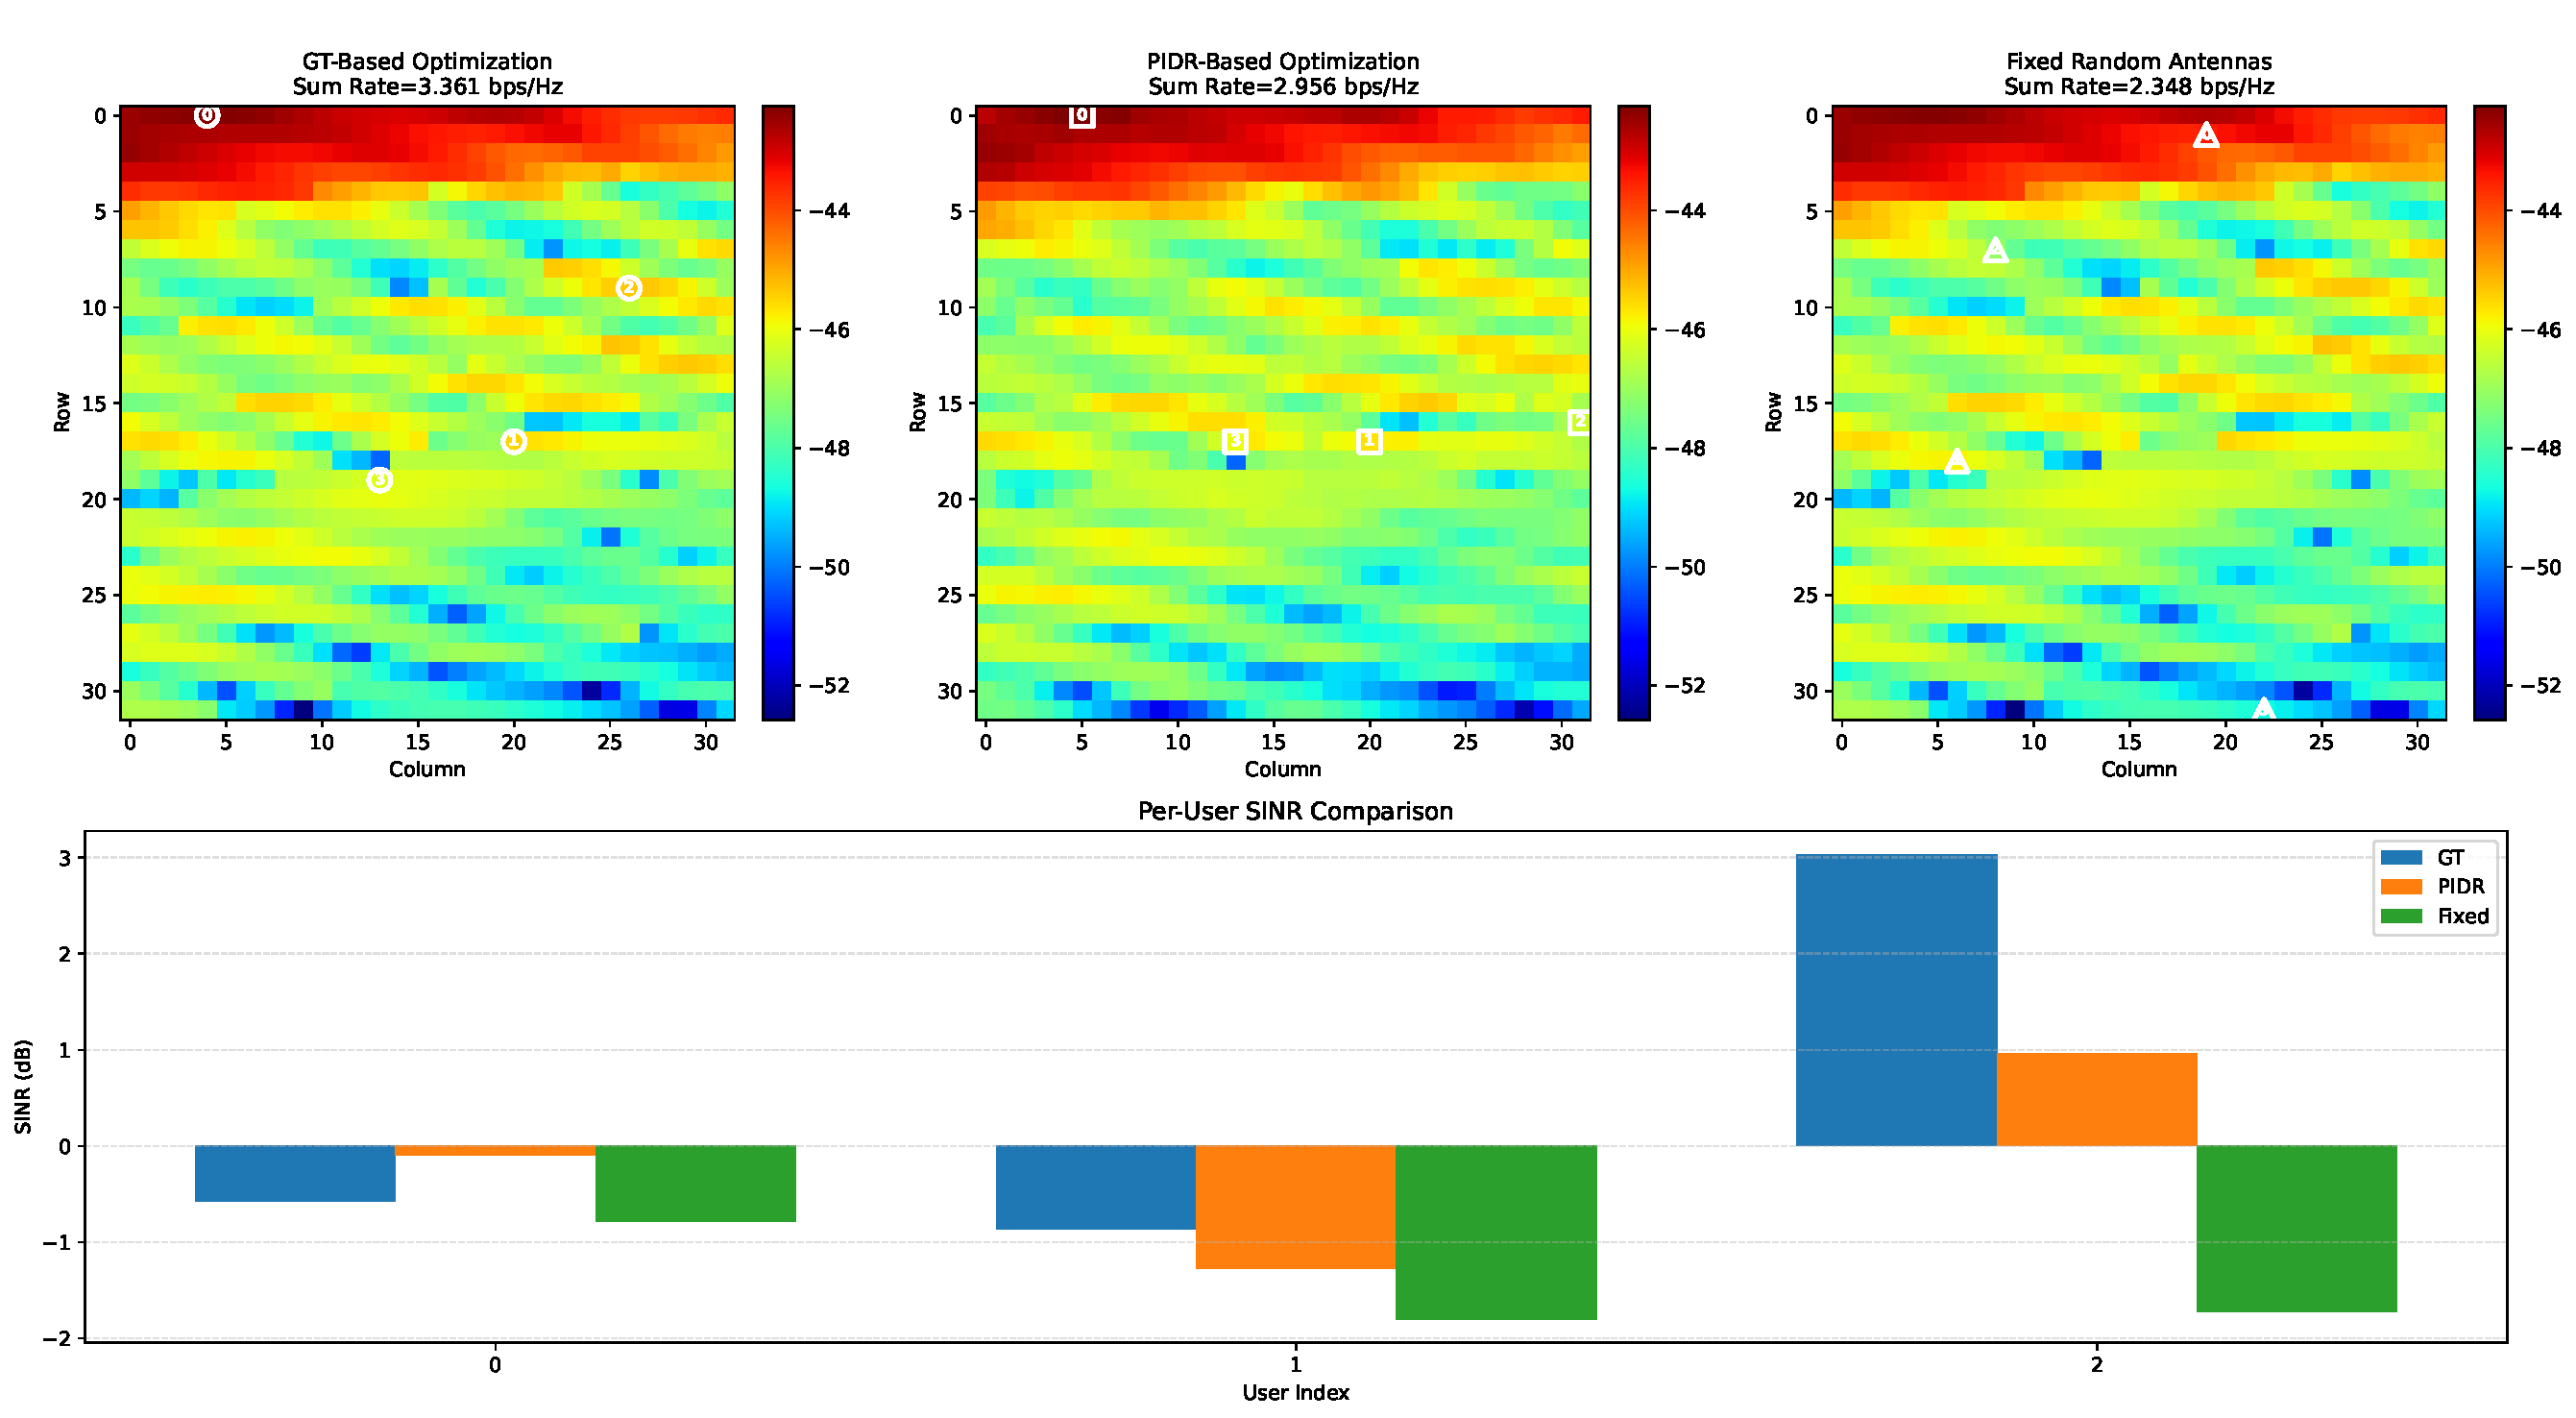
\includegraphics[width=0.32\textwidth]{figures/ma_multi_user_sr.pdf}}
	\hfill
	\subfloat[Field response]{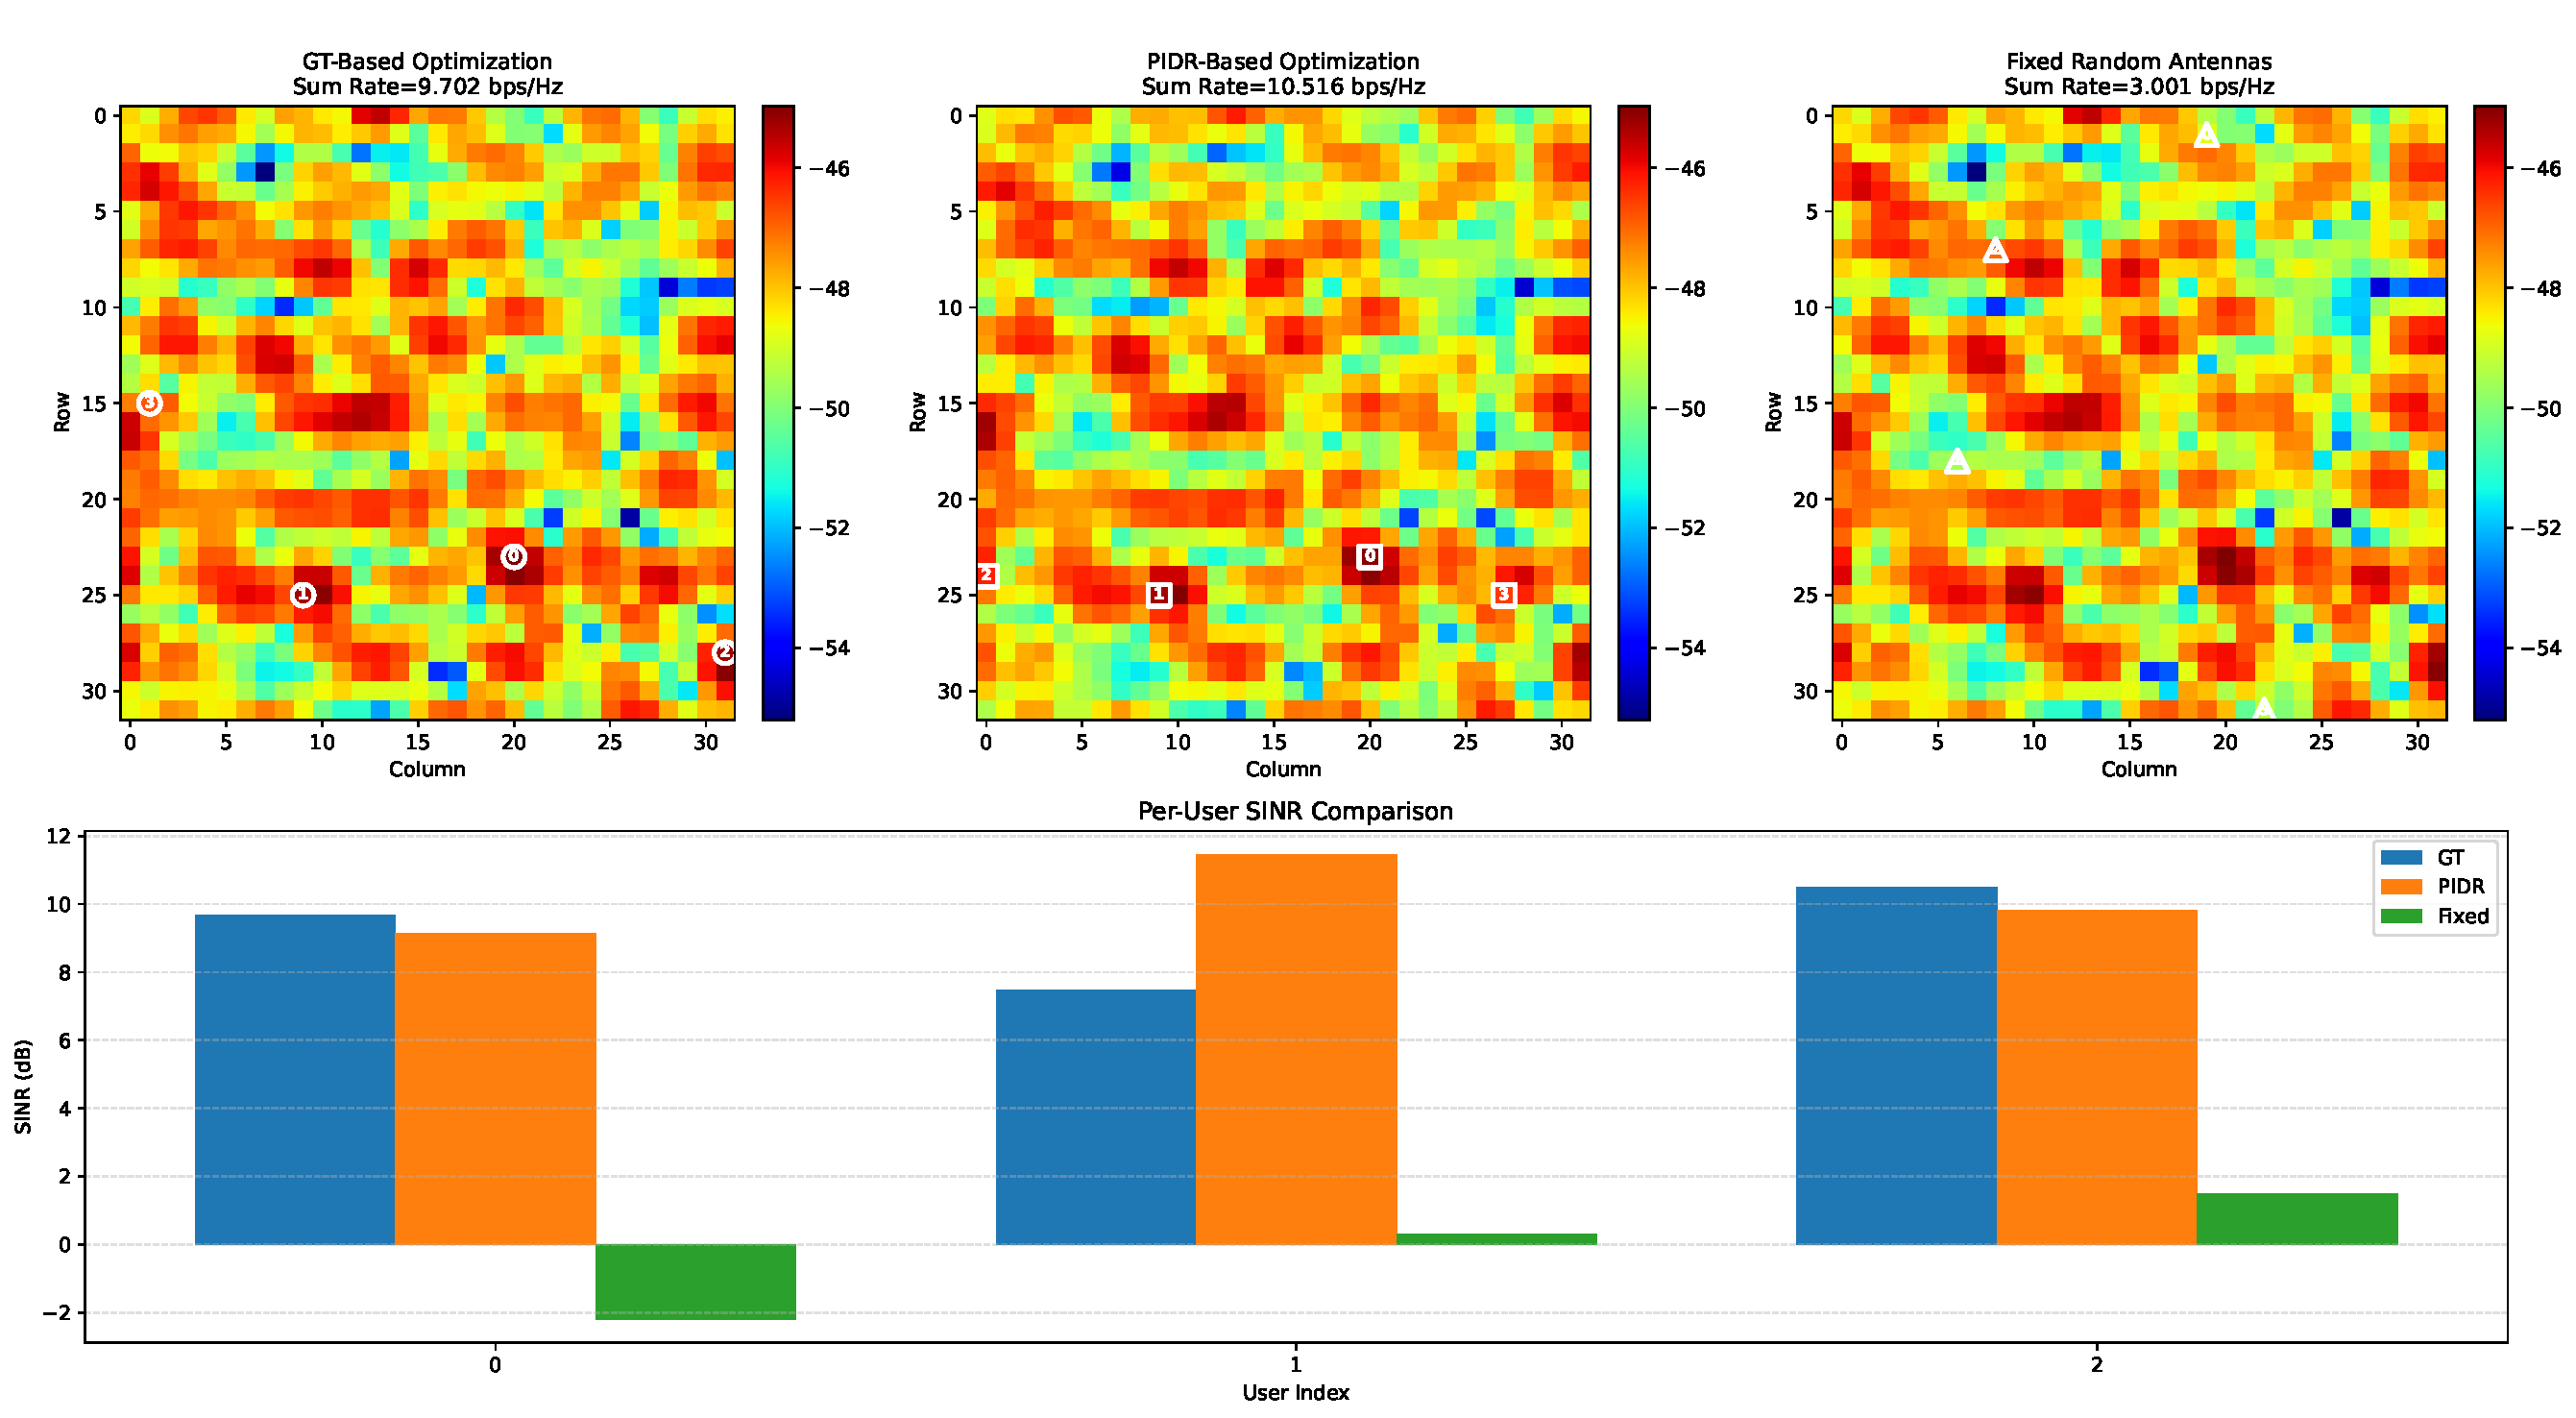
\includegraphics[width=0.32\textwidth]{figures/ma_multi_user_fd.pdf}}
	\hfill
	\subfloat[EM simulation]{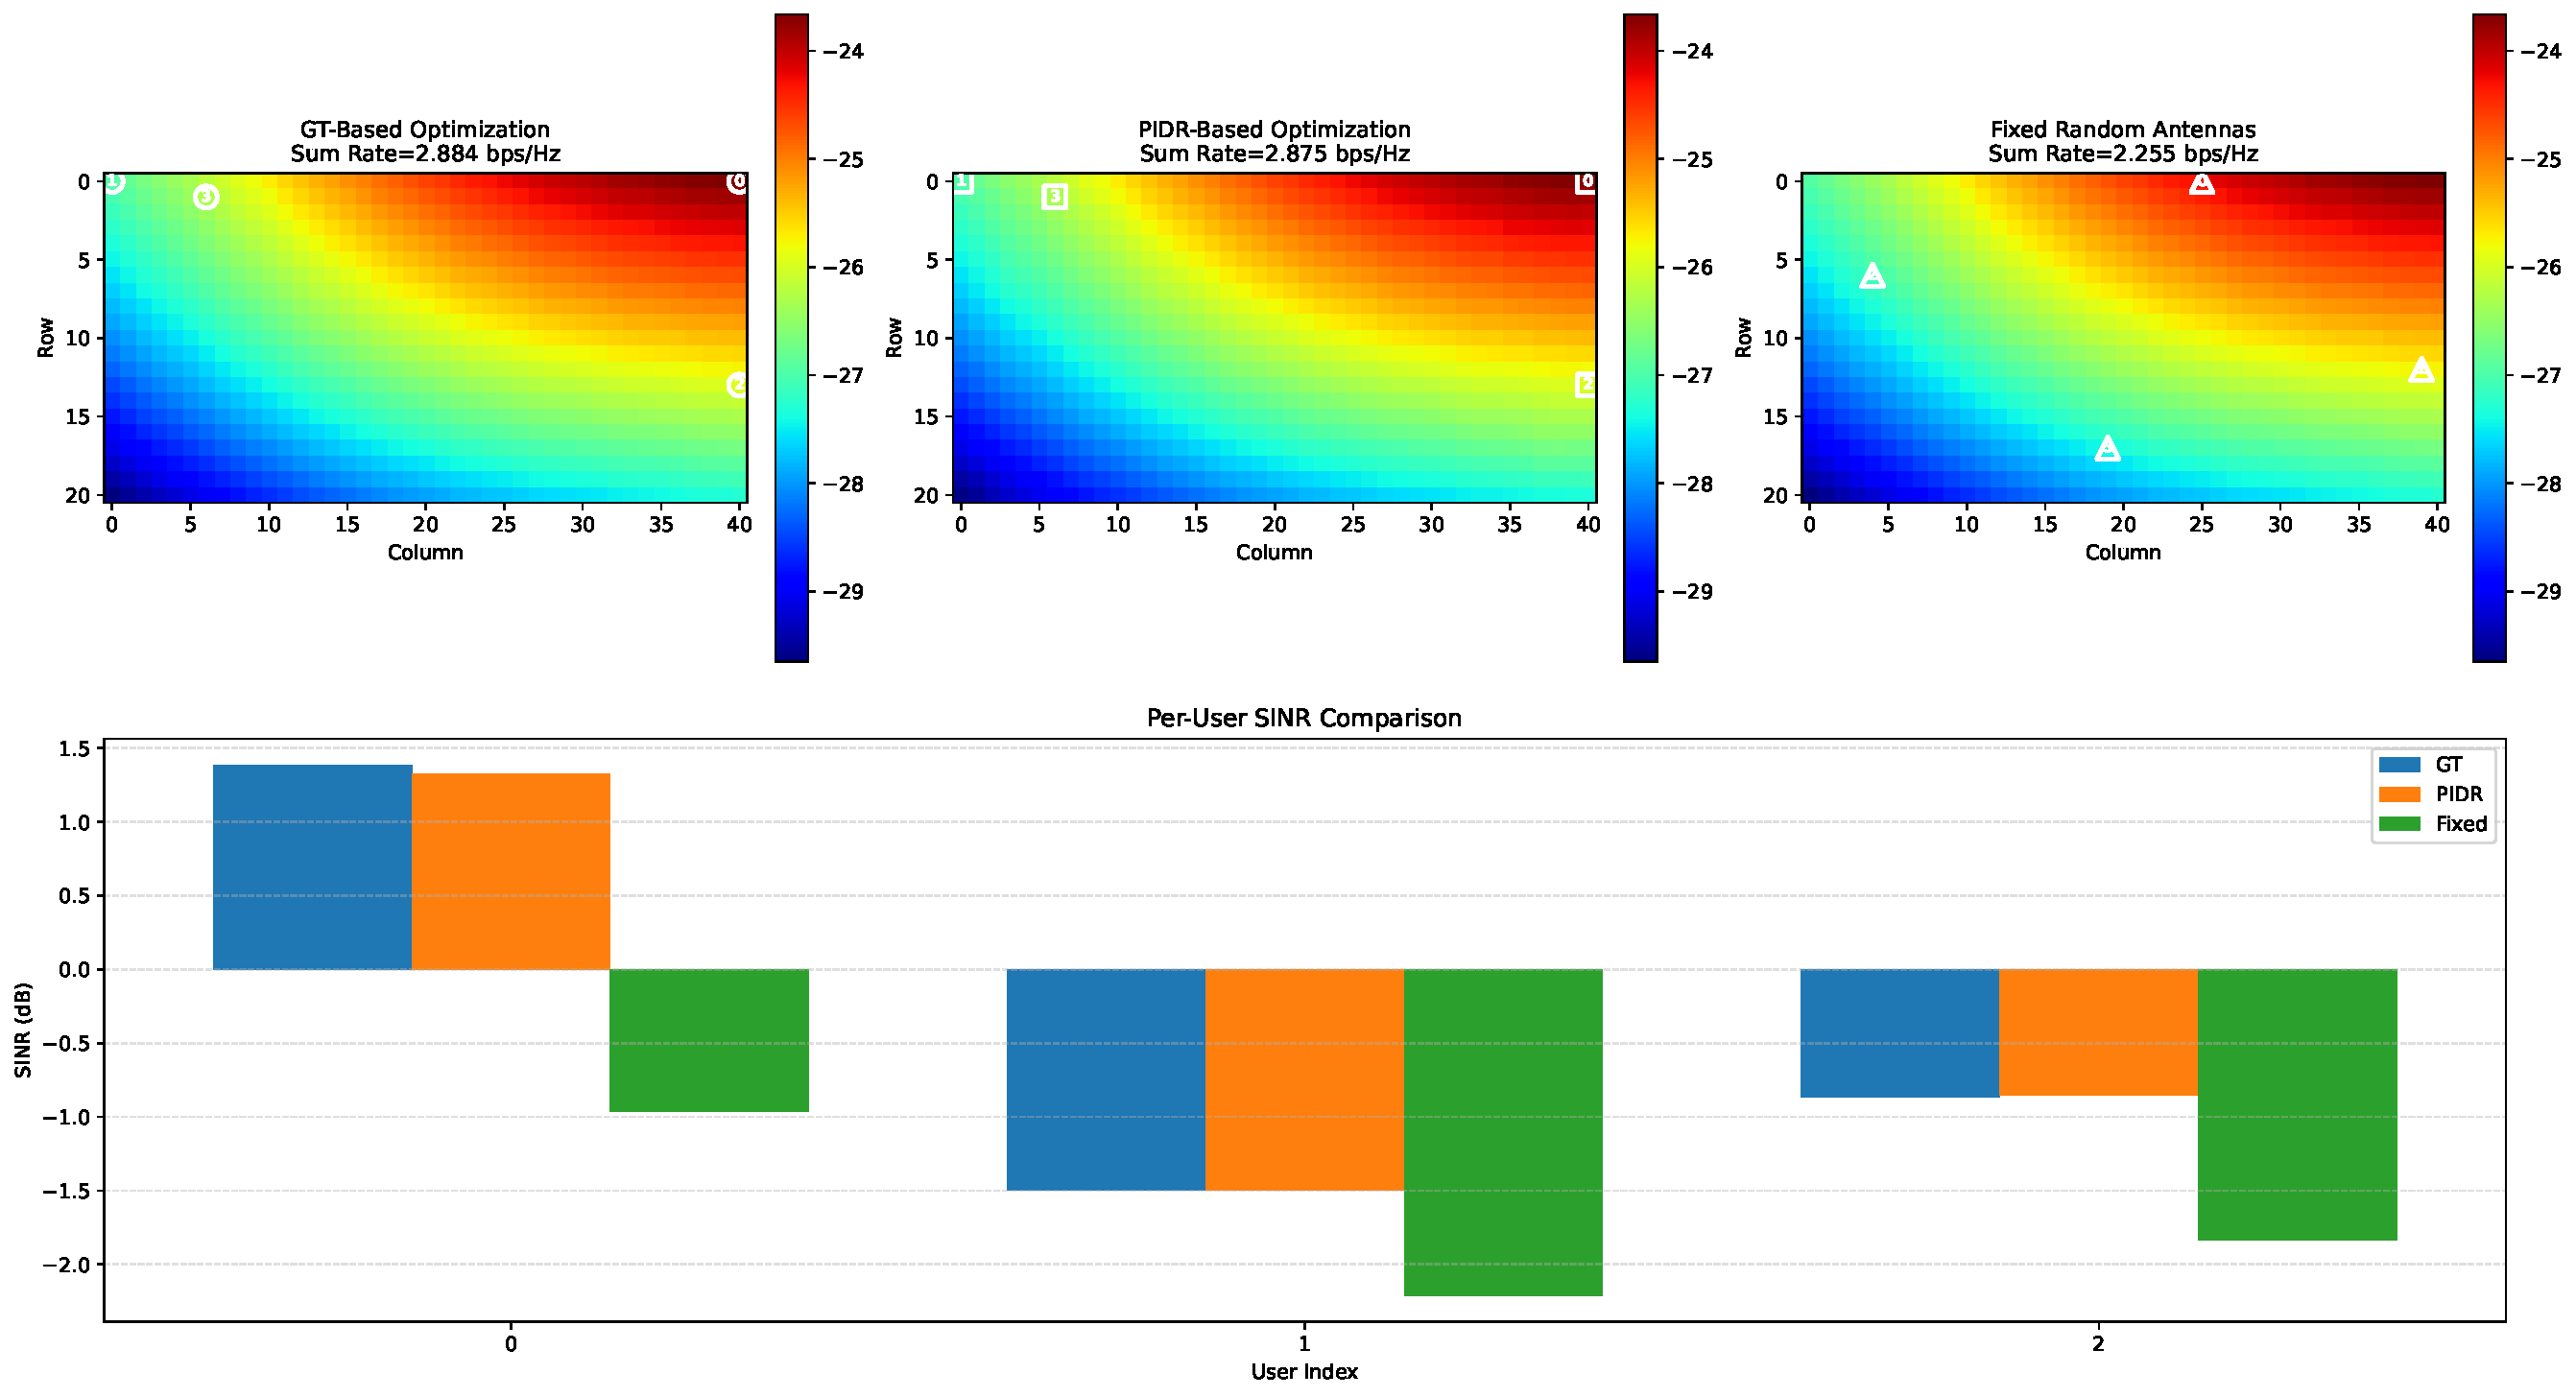
\includegraphics[width=0.32\textwidth]{figures/ma_multi_user_el.pdf}}
	\caption{\protect\centering MA position optimization results for multiple users on three datasets.}
	\label{fig:ma_multiuser_comparison}
\end{figure*}

The GT based optimizer uses the complete map as a reference and selects antenna locations in high gain regions. The optimizer using PIDR maps selects similar regions in the examples shown in Fig.~\ref{fig:ma_multiuser_comparison}.

The fixed random deployment does not use the channel maps and gives lower rates in the reported experiments. The gap is larger in the tested case with more movable antennas, where position selection has more effect on the joint channel.

The rate results show that the reconstructed maps retain information useful for MA position selection. Optimization using PIDR maps outperforms fixed random placement on all three datasets and approaches the GT based reference on the Sionna RT and EM simulation datasets.

\FloatBarrier

\subsection{Discussion}

The experiments show three main patterns. First, diffusion gives lower errors than the standalone PINN when observations are sparse or locally concentrated. Second, refining the diffusion result improves most reconstruction metrics by using the coordinate and propagation inputs. Third, the position optimization results depend on the spatial ordering of candidate locations as well as the average reconstruction error.

PIDR-Net has two main limitations. It requires offline training maps that represent the deployment conditions, so an untested environment shift may reduce accuracy. Reverse diffusion also requires more inference steps than interpolation or a single pass regressor. Reduced step sampling or distillation could lower this cost in future work.

\section{Conclusion}
\label{sec:conclusion}

This paper proposed PIDR-Net for reconstructing sparse complex CSI maps over a 2D MA movement region. Conditional diffusion first fills the unmeasured entries, and a compact PINN then corrects the estimate using coordinates and a learned propagation prior. Measured entries are retained, and the amplitude channel is kept consistent with the real and imaginary channels during reverse sampling. PIDR-Net achieves the best reported reconstruction metrics on the three evaluated datasets and under most tested sampling settings. Position optimization using the reconstructed maps also gives higher communication rates than fixed random antenna placement in the reported experiments.


\bibliographystyle{IEEEtran}
\bibliography{references} 



\end{document}
